% !TeX program = xelatex
% 初稿 2026-11-12。来源与待核对事项见 README_初稿.md。
% 本模板使用 xeCJK 和 TTF 字体，pdfLaTeX 不能编译。
\ifdefined\XeTeXversion\else
  \errmessage{HUST thesis requires XeLaTeX. In Overleaf Settings, select XeLaTeX, not pdfLaTeX}
  \expandafter\endinput
\fi
\documentclass[draftformat,mathCMR]{HUSTthesis}
\ifdefined\ThesisFastPreview
  \setkeys{Gin}{draft}
\fi
\usepackage{setspace}
\usepackage{bm,mathtools,tabularx,multirow,makecell,longtable}
\usepackage{algorithm,algorithmic}
\usepackage{float}
% TikZ 图已预编译为矢量 PDF；正文编译无需加载 PGF/TikZ。
\usepackage{placeins}
\IfFontExistsTF{Times New Roman}{\setmainfont{Times New Roman}}{\setmainfont{TeX Gyre Termes}}
\IfFontExistsTF{Arial}{\setsansfont{Arial}}{\setsansfont{TeX Gyre Heros}}
\newcolumntype{Y}{>{\centering\arraybackslash}X}
\newcolumntype{P}[1]{>{\centering\arraybackslash}p{#1}}
\DeclareMathOperator*{\argmax}{arg\,max}
\DeclareMathOperator*{\argmin}{arg\,min}
\DeclareMathOperator{\TopK}{TopK}
\DeclareMathOperator{\nnz}{nnz}
\DeclareMathOperator{\clip}{clip}
\DeclareMathOperator{\round}{round}
\newcommand{\norm}[1]{\left\lVert#1\right\rVert}
\newcommand{\abs}[1]{\left|#1\right|}
\newcommand{\hbalance}{\ensuremath{\mathrm{H}^{2}\mathrm{Balance}}}
% 图、图题与对应正文作为整体分页；图间始终保留说明文字。
\newcommand{\thesisfig}[5][0.88]{\FloatBarrier\par\addvspace{10pt}\penalty0\noindent
\begin{minipage}{\linewidth}\centering
\IfFileExists{figures/#2.tex}{\includegraphics{#2}}{%
\includegraphics[width=#1\linewidth,height=.64\textheight,keepaspectratio]{#2}}
\captionof{figure}{#3}\label{#4}
\parbox{\linewidth}{\setlength{\parindent}{2em}\indent #5\par}
\end{minipage}\par\addvspace{10pt}}
\floatname{algorithm}{算法}
\renewcommand{\algorithmicrequire}{\textbf{输入：}}
\renewcommand{\algorithmicensure}{\textbf{输出：}}
\numberwithin{algorithm}{chapter}
\setlength{\emergencystretch}{2em}
\hypersetup{pdftitle={面向稀疏矩阵计算的近似计算与软硬件协同加速技术研究},pdfauthor={翟嘉琪},bookmarksnumbered=true}
\begin{document}
\graphicspath{{figures/}}
\frontmatter
% !TeX root = ../main.tex
\ctitle{面向稀疏矩阵计算的近似计算与软硬件协同加速技术研究}
\xuehao{D202381438}\schoolcode{10487}
\csubjectname{计算机科学与技术}\cauthorname{翟嘉琪}
\csupervisorname{石宣化}\csupervisortitle{教授}\miji{}
% 原模板的具体答辩日期未经核实，初稿留待确定。
\defencedate{待确定}\grantdate{}\chair{}
\firstreviewer{}\secondreviewer{}\thirdreviewer{}
\etitle{Approximate Computing and Hardware--Software Co-Design for Accelerating Sparse Matrix Computations}
\edegree{Doctor of Philosophy in Engineering}
\esubject{Computer Science and Technology}\eauthor{ZHAI Jiaqi}
\esupervisor{Prof. SHI Xuanhua}\edate{2027}
\dctab{\begin{tabular}{|P{1.3cm}|P{2cm}|P{2cm}|P{5.2cm}|}\hline
角色&姓名&职称&单位\\\hline
主席&&&\\\hline 委员&&&\\\hline 委员&&&\\\hline 委员&&&\\\hline 委员&&&\\\hline
\end{tabular}}
\cabstract{
稀疏矩阵计算广泛存在于信息检索、推荐系统及科学工程计算中，是高性能计算系统的重要基础。以稀疏矩阵--向量乘法为核心的执行流程具有算术强度低、访存不规则及负载分布不均等特征，计算性能常受数据传输与执行组织限制。传统优化主要围绕既定计算精度与计算范围提高执行效率，较少利用不同计算阶段、数据区域与运行状态之间的计算需求差异。近似计算为减少冗余运算和数据访问提供了机会，但其收益同时受计算质量、额外决策开销与底层执行效率影响，因而需要联合设计近似计算机制与软硬件执行系统。

本文围绕稀疏矩阵计算中的计算精度冗余、计算范围冗余和动态精度需求，研究三类近似计算与协同加速方法。首先，通过分析 Top-K 稀疏检索与共轭梯度迭代求解的计算特征，区分候选保持、召回率和数值收敛三种质量要求，建立以计算需求识别、近似计算决策和协同执行为核心的研究思路。在此基础上，开展以下研究。

针对全量高精度 Top-K 稀疏计算的访存开销，提出低比特分层计算方法及加速系统 AccelES。采用 INT6 近似计算筛选候选，并结合 ReSparse 非零元素剪枝降低第一阶段的数据量，仅对候选执行 FP32 重算。设计 Ultra-CSR 与 Random-CSR，分别适配低精度流式扫描和高精度按行访问，并以 FPGA 异构计算核心实现两阶段协同执行。在原论文的五个真实语料派生数据集和六个人工数据集上，完整重算配置相对所选 FPGA、GPU、CPU 基线分别取得 3.4、2.5 和 153.3 倍加速，实验中的最大候选保持率损失为 0.95\%。

针对低比特阶段仍需遍历全量候选的问题，提出结构感知选择性计算系统 ParetoES。采用 Spherical K-means++ Refine 构建方向敏感的候选簇，通过簇探测控制实际计算范围；在继承低比特量化与稀疏压缩的基础上，设计自适应簇探测引擎、分布式微型排序单元和分层热点负载均衡策略，将搜索空间缩减转化为并行执行收益。在五个数据集、Recall@100 为 0.8 至 1.0 的评估区间内，相对 AccelES 的平均吞吐提升为 2.27 倍，相对 CPU 和 GPU 基线的最高吞吐提升分别约为 540 倍和 79 倍。

针对迭代状态变化导致的动态精度需求，提出状态感知混合精度求解系统 EvoCG。通过强化学习将搜索方向的局部数值特征映射为 FP64、FP32 和 BF16 精度决策，结合 Tile-CSC 数据布局和统一的线程束计算内核实现异构精度执行，并采用设备端策略推理、区间复用及 CUDA Graph 降低运行时开销。在 47 个对称正定矩阵上，采用矩阵专属离线训练策略时，相对 cuSPARSE、PETSc、Ginkgo、Mille-FP64 和 Mille-Mixed 的几何平均加速比分别为 2.52、3.06、2.48、1.93 和 6.99。其中，Mille 系列比较仅统计其实现成功求解的矩阵子集。相对相同执行基础上的全 FP64 配置，动态精度控制带来 1.28 倍几何平均加速，平均迭代次数增加 11.4\%，策略推理平均占在线求解时间的 1.09\%。

上述研究表明，在相应质量约束下，识别并利用计算需求差异能够减少稀疏计算的实际执行成本。低比特分层计算与结构感知选择性计算形成从降低单位计算成本到缩减计算范围的技术递进，状态感知混合精度则将研究拓展到具有误差传播和状态反馈的迭代过程。三项研究共同说明，近似计算机制必须与稀疏数据表示、并行执行架构及运行时调度相适配，才能形成端到端性能收益。
}
\ckeywords{稀疏矩阵计算；近似计算；软硬件协同设计；混合精度}
\eabstract{
Sparse matrix computations are fundamental to information retrieval, recommendation, and scientific computing. Workflows centered on sparse matrix--vector multiplication (SpMV) often suffer from low arithmetic intensity, irregular memory accesses, and load imbalance. Conventional optimizations improve the execution of a prescribed workload, while differences in precision requirements across stages, data regions, and evolving solver states create opportunities to reduce the workload itself. Realizing these opportunities requires approximate computation to be co-designed with sparse representations, parallel architectures, and runtime mechanisms.

This dissertation investigates three complementary problems: redundant high-precision computation, redundant candidate processing, and state-dependent precision requirements. First, AccelES introduces a two-stage Top-K SpMV workflow. INT6 computation and ReSparse pruning identify a compact candidate set, followed by FP32 recomputation. Ultra-CSR and Random-CSR support streaming screening and row-wise refinement, respectively, on a heterogeneous FPGA architecture. On the original evaluation workloads, the refinement configuration achieves reported speedups of 3.4, 2.5, and 153.3 over the selected FPGA, GPU, and CPU baselines, with a maximum observed candidate-retention loss of 0.95\%.

Second, ParetoES reduces the candidate range that still must be scanned by AccelES. It combines Spherical K-means++ Refine with configurable cluster probing, adaptive FPGA probing engines, distributed micro-sorters, and hierarchical hotspot balancing. Over five datasets and Recall@100 targets between 0.8 and 1.0, it improves average throughput over AccelES by 2.27 times. Its highest throughput improvements over the evaluated CPU and GPU baselines are approximately 540 and 79 times, respectively.

Third, EvoCG extends approximate computation to iterative sparse solvers whose numerical sensitivity changes with the Krylov state. A reinforcement-learning controller selects FP64, FP32, or BF16 for column-block-associated tiles. Tile-CSC and a unified warp-centric SpMV kernel support heterogeneous execution, while device-side policy inference, interval reuse, and CUDA Graph replay reduce runtime overhead. With matrix-specific offline training, experiments on 47 symmetric positive definite matrices show geometric-mean speedups of 2.52, 3.06, 2.48, 1.93, and 6.99 over cuSPARSE, PETSc, Ginkgo, Mille-FP64, and Mille-Mixed. Comparisons with the Mille implementations are restricted to the subsets on which those implementations complete successfully. Against the identical execution substrate using FP64 throughout, dynamic precision control provides a 1.28-times geometric-mean speedup, with 11.4\% more iterations on average and average online policy overhead of 1.09\%.

These studies use distinct quality criteria: candidate preservation, retrieval recall, and numerical convergence. They do not assume a universal error model. Together, they demonstrate that exploiting differences in computational requirements can reduce sparse execution costs when approximation decisions are matched to the data representation and execution system. The progression from hierarchical precision to selective computation is complemented by an extension to feedback-driven precision control in iterative solvers.
}
\ekeywords{Sparse matrix computation; Approximate computing; Hardware--software co-design; Mixed precision}

\makecover
\tableofcontents
\mainmatter
\raggedbottom
% !TeX root = ../../main.tex
\chapter{绪论}\label{chap:intro}
\section{研究背景与意义}
\subsection{稀疏矩阵计算及其典型应用}
稀疏矩阵通过只存储和处理非零元素，将原本由矩阵维度决定的计算与存储需求转化为由有效数据规模决定的开销。这一表示方式广泛用于科学工程计算、图分析和机器学习系统。随着问题规模增大，稀疏性使许多原本无法在有限内存中处理的问题成为可能；与此同时，非零元素分布的不规则性也使稀疏计算难以直接获得稠密计算所具备的数据复用与并行执行效率\cite{gao2024systematic}。

本文主要围绕稀疏矩阵--向量乘法（Sparse Matrix--Vector Multiplication，SpMV）及其关联执行流程开展研究。给定稀疏矩阵 $A$ 与向量 $x$，SpMV 计算 $y=Ax$。不同应用赋予这一算子不同的输出语义：在稀疏嵌入相似度检索中，系统通常只需要得分最高的少量候选；在共轭梯度（Conjugate Gradient，CG）求解中，SpMV 的结果参与后续残差与搜索方向更新，影响整个迭代过程。研究范围因此包含 Top-K 选择、候选重算与 CG 运行时等紧密相关的操作，但不覆盖全部稀疏矩阵算子。

稀疏嵌入将对象表示为少量有效特征组成的向量，可用于词语语义分析、信息检索和推荐。已有工作探索稀疏过完备词向量与稀疏神经检索，以表达语义信息并提高检索可解释性\cite{sparse_2015,spine_2018,formal2021splade}。对矩阵中的每个候选向量计算与查询向量的相似度，再提取 Top-K 结果，构成本文前两项研究的基本计算流程。本文采用的多组数据由经典词向量经稀疏化得到，具有特定的维度与数值分布；向现代高维词项检索场景拓展时，还需相应调整数据表示与执行结构。

CG 则面向对称正定线性方程组，通过递推构造搜索方向逐步求解\cite{hestenes1952,saad2003}。对大规模稀疏系统而言，每次迭代包含 SpMV、向量更新与内积归约，其时间开销由算子执行效率与迭代次数共同决定。由此，同一 SpMV 算子在检索和数值求解中呈现出不同的精度需求，也为研究具有不同质量语义的近似计算方法提供了代表性对象。

\subsection{稀疏矩阵计算的性能瓶颈}
与稠密矩阵乘法相比，SpMV 的每个非零元素通常只贡献一次乘法和一次加法，矩阵元素很难在同一次调用中获得高复用。除数值外，系统还必须读取列索引、行边界等元数据，并根据列索引间接访问输入向量。实际运行时间因而不仅取决于浮点运算能力，还受内存带宽、访问粒度和有效载荷比例限制。Roofline 模型将可达性能约束于计算峰值和带宽所能支持的运算速率，可用于解释这一现象\cite{williams2009roofline}。

不规则稀疏结构进一步增加并行执行难度。按行划分任务时，长行与短行的工作量差异容易导致线程束内部利用率不足；按非零元素划分任务时，又需要处理跨行归约及输出写入冲突。即使总数据量保持不变，不同矩阵也可能因行长度、列访问局部性和块结构不同而呈现不同性能\cite{li2014performance,xia2022comprehensive}。因此，提高峰值算力并不能自动解决稀疏计算瓶颈。

在 Top-K 检索中，算子后续的排序与结果维护还会增加数据往返和同步开销；在 CG 中，多个短内核之间的启动、全局归约和状态传递则可能进入关键路径。仅优化单次 SpMV 的吞吐并不足以说明应用受益，研究必须将 Top-K 结果生成或达到目标残差的完整过程纳入评估。

\subsection{近似计算的性能优化机会}
传统稀疏优化在保留既定数值精度与运算集合的前提下，改进数据布局、缓存和任务调度。近似计算进一步允许依据输出质量要求，改变实际参与计算的数据、数值位宽或执行次数。在检索任务中，排序只关注相对次序，高精度计算并非对每一行都具有同等价值；在迭代求解中，不同数值状态对局部运算误差的敏感程度也并不相同。

上述机会主要体现在三个方面：在计算阶段之间，通过低比特预筛与高精度重算分配精度预算；在数据区域之间，通过结构感知的候选选择缩减访问范围；在迭代状态之间，根据数值反馈动态调整局部精度。三者分别对应本文关注的计算精度冗余、计算范围冗余和动态精度需求。它们在实现上相互关联，例如低比特筛选同时缩小高精度计算范围，动态混合精度同时涉及空间划分与时间调度。

近似计算的价值在于减少实际执行成本，而不是单纯降低数值表示精度。若低位宽数据仍采用宽字存储，或剪枝后引入的零散访问无法形成有效传输，则算法层面的简化可能无法转化为加速。这要求近似策略与底层执行机制共同设计。

\subsection{近似计算与软硬件协同加速面临的挑战}
首先，近似机制需要满足具体任务的质量约束。低比特计算可能改变 Top-K 边界附近的候选次序，FP32 重算能够校正保留候选的得分，但候选遗漏仍会限制最终召回率。簇级选择通过排除部分数据区域减少访问，其效果体现为召回率与吞吐率的权衡。CG 中的低精度扰动则沿迭代递推传播，影响残差、搜索方向及收敛过程。因此，候选保持率、检索召回率和数值收敛性分别构成三类方法的质量评价依据。

其次，需要解决近似决策引入的执行不规则性。低比特筛选与高精度重算对应不同的访问方式；选择性簇探测使各核工作量依赖查询分布；Tile 级混合精度则使相邻任务的计算成本不同。如果数据表示和资源分配仍沿用原有均匀执行假设，近似计算产生的收益就会被额外索引、调度和同步开销抵消。

最后，端到端评估需要区分近似机制与执行优化的贡献。跨平台加速同时受到工作量缩减、数据表示和硬件实现的影响，单一加速比难以解释各项技术的独立作用。本文在匹配质量目标的基础上，结合相同执行基础上的消融实验与额外开销分析，考察近似决策、数据布局和运行时优化的收益。对于强化学习精度控制，还进一步分析离线训练成本、策略复用条件和迁移效果。

\section{国内外研究现状}
\subsection{稀疏矩阵计算的异构加速技术}
CPU 稀疏计算通常依靠多线程划分、向量化和数据重排提高缓存利用率。矩阵重排可以改善局部性，但其效果取决于稀疏结构以及预处理成本是否能被重复调用摊销\cite{trotter2023bringing}。对 Top-K 检索而言，稀疏乘法与候选维护融合有助于避免输出全部中间结果，但仍需面对内存带宽与线程间负载分布的约束。

GPU 通过大量线程隐藏访存延迟，是 SpMV 的重要执行平台。早期研究系统讨论了稀疏格式与吞吐型处理器的匹配关系\cite{bell2009}，CSR5 等格式进一步通过分块和元数据设计改善跨平台并行效率\cite{csr5_2015}。cuSPARSE 提供常用稀疏运算接口\cite{cusparse_2010}，相关研究还通过自适应线程配置、格式选择和负载均衡优化不同矩阵上的性能\cite{adaptive_2020,gao2024revisiting,anzt2020load}。这些工作说明稀疏计算性能高度依赖结构与执行方式的匹配。

FPGA 能够围绕特定数据流构建并行解码、乘加和归约电路。HBM 的多通道结构为流式稀疏计算提供较高并发带宽，但通道分配、数据打包和片上缓冲仍需协同设计\cite{shuhai_2020}。Serpens 和 Sextans 分别针对 SpMV 与稀疏矩阵--稠密矩阵乘法设计面向存储的执行结构\cite{serpens_2022,sextans_2022}。针对 Top-K SpMV 的 FPGA 工作引入流式压缩和片上候选维护\cite{scaling_2021}，为本文研究提供了直接比较对象。现有异构优化为执行层奠定基础，但未必充分利用应用输出对计算精度和计算范围的容忍度。

\subsection{低精度与混合精度计算优化技术}
低精度计算通过减少数值位宽降低存储和传输开销，并提高特定硬件上的计算吞吐。对于相似度检索，量化误差影响的是得分与排序边界，其允许程度取决于候选分数间隔和最终召回要求。产品量化等方法通过压缩向量表示降低近似最近邻检索成本\cite{jegou2010product}；低比特定点运算则可与稀疏数据流及 FPGA 自定义位宽直接结合。

数值线性代数中的混合精度需要更严格地考虑误差传播。已有综述总结了低精度运算、迭代改进和高精度校正的组合方式\cite{abdelfattah2021,higham2022}。不精确 Krylov 理论分析矩阵--向量乘法扰动对收敛和可达精度的影响，为在迭代中使用低精度提供理论基础\cite{simoncini2003,bouras2005,eshof2004}。这些理论并不直接给出适合具体 GPU 的最低运行时间精度配置，数值可行性与硬件性能之间仍存在设计空间。

Mille-feuille 将 Tile 级混合精度与单内核 CG 执行结合\cite{yang2024mille}，Callipepla 研究面向 CG 的流式指令集和混合精度 FPGA 加速\cite{song2023callipepla}。近期工作还探索通过强化学习选择 CG 精度\cite{chen2025rl}。与静态精度方案或外部参数调优相比，本文第五章关注迭代内状态反馈如何驱动局部精度决策，以及如何使决策开销足够低，从而改善完整求解时间。

\subsection{基于剪枝的选择性计算优化技术}
候选筛选的目标是将有限计算预算集中到更可能影响结果的数据区域。近似最近邻方法包括局部敏感哈希、倒排索引、产品量化和图索引等\cite{datar2004locality,jegou2010product,malkov2018efficient}。Faiss 将多种索引与 CPU、GPU 执行实现集成，使召回率与查询吞吐之间的权衡成为可调参数\cite{douze2024faiss}。这类系统表明，避免遍历所有候选是提高检索效率的重要途径。

稀疏向量的方向、幅值及非零支撑集共同决定候选之间的关系。将针对稠密数据设计的聚类和执行方案直接迁移到稀疏场景，可能受到簇代表方向偏移、数据密度差异以及热点访问的影响。与此同时，元素级剪枝和簇级候选排除分别作用于向量内部与向量集合，两者的误差来源及成本结构不同，必须在同一质量目标下联合评估。

本文第三章以低比特全量筛选和元素级剪枝降低计算成本，第四章进一步使用方向敏感聚类约束候选范围。后者继承前者的低位宽与数据格式基础，但新增簇选择、动态探测和多核热点均衡机制，构成计算范围层面的技术拓展。

\subsection{近似计算的软硬件协同优化技术}
算法与硬件协同设计要求同时考虑数据组织、执行粒度与可实现的并行结构。在向量检索中，已有研究通过联合设计索引与硬件流水线提高搜索效率\cite{jiang2023co}；在稀疏运算中，格式与调度联合优化能够根据实际负载选择执行方案\cite{won2023waco}。这些研究说明，算法减少的运算量只是潜在收益，系统能否减少内存事务和同步等待决定了实际收益。

迭代求解中的协同优化还涉及算子间状态传递。融合内核能够减少重复读写和内核启动\cite{aliaga2015,rupp2016}，但融合程度增加后也可能引入设备端同步和调度约束。混合精度进一步改变各任务的成本，使数据布局与任务分配需要重新设计。因此，本文将近似决策与执行优化分别建模、联合实现，并通过相同执行基础上的平台消融检查两者的独立贡献。

% !TeX root = ../../main.tex
\subsection{表示学习与检索计算需求的演变}
词向量研究通过向量空间关系表达词语的语言规律\cite{mikolov2013linguistic}，相关综述进一步讨论超越静态词嵌入的表示方法\cite{incitti2023beyond}。Transformer、自监督语言建模和 BERT 等工作改变了向量产生方式\cite{vaswani2017attention,radford2018improving,devlin2018bert}，LMMS 则体现上下文语义表示在词义任务中的应用\cite{loureiro2022lmms}。这些研究影响检索输入的维度和分布，但表示模型与底层稀疏检索分别影响语义质量和执行成本，两者的收益需要在相应系统边界内评价。

从系统视角看，表示学习与相似度计算之间存在接口。编码器决定向量的维度、范数和稀疏支撑，检索系统则决定候选如何存储与扫描。对本文而言，需固定编码器与稀疏化方法，再比较后端执行；若同时改变表示模型，召回变化将混合语义表示误差和算子近似误差。因此，前两项工作的实验以既定稀疏矩阵为输入，不将硬件加速等同于完整表示学习流程的加速。

传统词项检索以 Okapi 等模型为代表\cite{1995BM25}，神经稀疏检索则探索从重排序到可索引表示的转换\cite{zamani2018neural,bai2020sparterm}。SPLADE 系列进一步研究稀疏词项扩展与效率权衡\cite{formal2021splade_v2,formal2024towards}。这些任务与本文的共同点是候选计算具有稀疏结构，但特征维度、查询稀疏性和得分分布未必相同。特别是词表维度远大于1024 的设置，不能直接套用本研究的10 位列索引和全量片上查询复制。

稠密段落检索、混合表示检索和多阶段重排序形成另一条研究路线\cite{karpukhin2020dense,chuang2024information,xu2023hybrid,sasazawa2023text}。这些系统通常将快速召回与精细比较分开，说明阶段间质量要求可以不同。本文借鉴的是这种阶段分工思想，具体实现仍以稀疏 SpMV 和候选集合为对象。应区分向量层面的 Recall@K 与重排序后的最终任务指标，避免用一个指标替代完整任务质量。

\subsection{推荐与检索增强应用中的候选计算}
协同过滤和基于物品的推荐方法为大规模相似度计算提供了早期应用背景\cite{goldberg1992using,sarwar2001item}。深度推荐、图推荐及强化学习推荐综述表明，实际系统往往同时涉及表示生成、候选召回和排序决策\cite{chen2020survey,zhang2021artificial,wang2021graph,afsar2022reinforcement}。因此，本文选择 Top-K 稀疏计算作为明确的系统边界，先验证这一核心流程的成本与质量，再讨论它与上层系统的可能联系。

推荐任务还存在多样性、知识增强和解释性等目标。DGRec 关注多样化嵌入，GHRS 研究图混合推荐，知识增强 Top-K 研究引入特定表示空间\cite{yang2023dgrec,darban2022ghrs,ma2021knowledge}；利用评论和细粒度方面的推荐工作则强调结果解释\cite{Amazon_Product_Reviews_2019}。这些目标表明，基于既定内积的 Top-K 计算只覆盖候选选择环节，推荐公平性、多样性和用户满意度仍取决于上层模型与排序策略。

工业研究讨论嵌入式搜索、兴趣建模和 CPU 推荐计算优化\cite{huang2020embedding,shen2022deep,jain2023optimizing}。矩阵分解与神经协同过滤的比较也强调一致基线的重要性\cite{rendle2020neural}。本文据此保持比较双方的数据、目标召回和计时范围一致；对于跨平台实现差异，则以消融而非单一加速比解释。生成式检索与推荐综述提供更广的系统视角\cite{rajput2023recommender,huang2024comprehensive}，但其执行流程与显式向量 Top-K 存在差异，属于后续适配方向。

检索增强生成将外部候选引入生成模型\cite{lewis2020retrieval,izacard2020leveraging}，混合检索和多分区检索进一步改变召回组织\cite{sawarkar2024blended,wang2024m}。在多模态场景中，晚交互、文档截图嵌入与视觉语言检索研究形成不同的相似度结构\cite{lin2023fine,ma2024unifying,zhan2025elip}。本文不把这些任务全部归约为完全相同的稀疏 SpMV，而是指出只有在上层计算能够明确映射为本文接口时，底层结果才可用于分析应用加速。

\subsection{稀疏格式、重排与执行映射的研究维度}
稀疏格式研究的核心是决定哪些结构信息显式存储，以及如何将其转化为并行任务。CSR2 以 SIMD 加速为背景\cite{bian2020csr2}，ARM 众核上的稀疏计算研究说明布局和执行映射具有平台相关性\cite{ZHENG2023103035}。GPU 算法设计和异构处理器评估则从不同实现角度分析稀疏及图计算内核\cite{chu2023efficient,zhang2019performance}。这些工作共同提示，仅以存储字节数评判格式是不充分的，解码、归约和线程利用率同样重要。

FPGA 相关研究覆盖能效稀疏 BLAS、数据复用压缩、重排和 Roofline 指导优化\cite{dorrance2014scalable,li2023efficient,li2021optimized,favaro2023optimizing}。HLS 研究关注高层综合表达与 HBM 平台之间的实现路径\cite{du2022high}，Vitis 稀疏库提供工程实现参考\cite{vitis_library}。本文将这些路线与应用语义驱动优化区分：前者改进给定工作量的执行，后者进一步改变哪些高精度数据需要读取，两者可以叠加而非相互排斥。

稀疏矩阵乘法与图神经网络加速还涉及不同的数据复用结构。ACES、HotTiles、SGCN 及 SIGMA 分别围绕执行流、异构资源、压缩特征或灵活互连展开研究\cite{ACES,gerogiannis2024hottiles,yoo2023sgcn,qin2020sigma}。这些工作提供相关体系结构思想，但 SpMM、图卷积与 SpMV 的算术强度和复用机会不同，本文不直接借用其峰值加速比评价本系统。FSPA 则提供另一种器件与计算组织背景\cite{zhang2023fspa}，进一步说明算法相同并不意味着实现约束相同。

编译器可通过稀疏中间表示组织算子与调度\cite{yang2023spmmplu}，近存多路归并可用于稀疏转置和数据流变换\cite{feng2022menda}。本文的格式转换目前主要在离线完成，后续可将固定格式和阶段切换关系显式表达为编译约束，使候选筛选、重算和混合精度的资源选择更易自动化。但这种自动化需要同时建模质量条件，不能只优化稀疏循环的执行顺序。

\subsection{低精度硬件与应用近似的区别}
低精度研究不仅涉及数值截断，还包括权重表示、缩放、异常值处理和硬件指令映射。OPTQ、INT8 语言模型计算和8 位 Transformer 研究提供了相关实例\cite{frantar2023optq,dettmers2022gpt3,yu20248}。模型蒸馏与高效神经网络处理则从更广的计算简化角度展开\cite{sanh2019distilbert,sze2020efficient}。这些工作作为邻近研究用于说明降低成本的不同层次，不直接作为本文 CG 误差可接受性的证据。

推荐推理的低精度硬件研究说明，数值格式选择应与目标应用和执行平台协调\cite{deng2021low}。打包 SIMD 指令相关工作提供位级并行组织的背景\cite{miyaoka2002algorithm}，长度自适应 Transformer 协同设计则体现输入相关执行预算的思想\cite{peng2022length}。本文采用 INT6 的关键条件是固定总线和可定制电路，并不是认为6 位在所有硬件或任务上天然优于8 位。

Top-K 稀疏特征问题中的多 GPU 混合精度研究\cite{sgherzi2022mixed}，与本文的检索 Top-K 和 CG 具有部分计算机制上的联系，但输出语义和误差传播方式不同。相关方法的适用性取决于数值对象及其输出语义。本文在比较近似方案时始终先说明数值对象、质量约束与执行范围，再讨论位宽、并行度及性能。

\subsection{软件基础、系统边界与可复现评估}
MKL、cuSPARSE、Cusp 及 Thrust 等软件提供不同层次的稀疏算子、并行算法和结果选择接口\cite{wang2014intel,cusp,thrust_docs}。Faiss 及 GPU 大规模相似度搜索研究提供向量索引与搜索实现\cite{faiss,johnson2019billion}，\texttt{sparse\_dot\_topn}提供稀疏乘法与 Top-N 候选计算接口\cite{sparsedottopn}。这些工具的支持数据类型、输出语义和可配置参数不完全相同，应在实验中记录实际使用路径，而不是仅列出库名。

向量数据库研究进一步涉及索引维护和系统管理\cite{2021milvus}。大数据学习及 MapReduce 相关工作说明离线准备、任务划分和重复执行构成独立成本\cite{zhou2017machine,dean2008mapreduce}。因此，本文区分一次性格式转换、在线查询和最终结果验证。对不能在相同实现路径上执行的比较，采用清楚的系统边界说明，并单独交代离线准备和结果验证的成本。

图嵌入研究中的稀疏投影和高阶结构表达\cite{chen2019fast,morris2020weisfeiler}也体现了“稀疏”在不同层次的含义。输入表示稀疏、矩阵结构稀疏和执行时动态跳过工作是不同概念。本文将三者分别落实到数据格式、候选决策和运行时机制，以减少术语混用，并使相关研究与具体技术贡献形成可检验的对应关系。

\section{研究内容与主要贡献}
本文研究的核心问题是：如何利用不同计算阶段、数据区域和运行状态的计算需求差异，通过近似计算及软硬件协同设计降低稀疏计算的实际执行成本？图\ref{fig:roadmap}展示全文研究内容及相互关系。
\begin{figure}[htbp]\centering
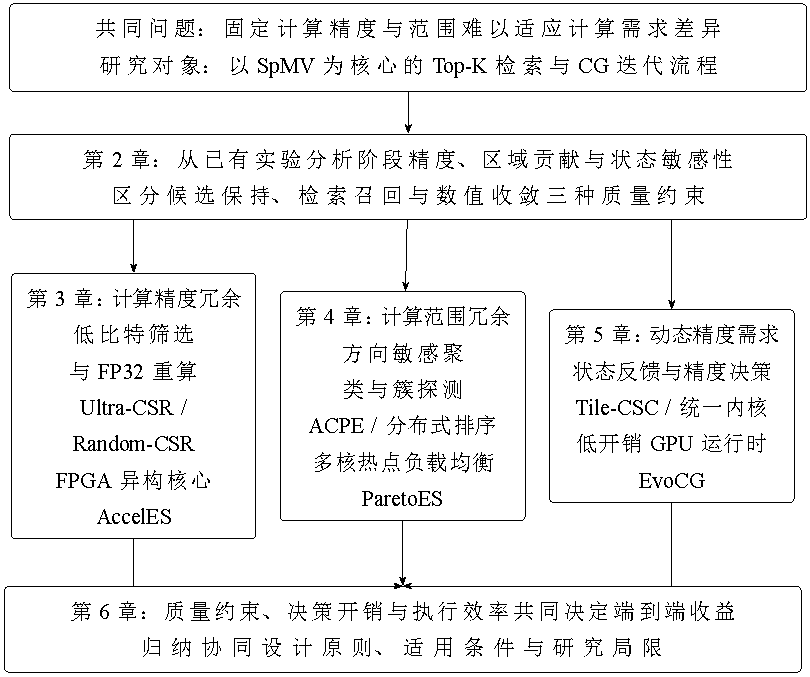
\includegraphics{roadmap.pdf}
\caption{全文研究内容与组织关系}\label{fig:roadmap}
\end{figure}

\subsection{面向计算精度冗余的低比特分层计算方法}
针对大量候选不需要高精度得分却仍参与全量浮点计算的问题，提出 AccelES\cite{jqzhai2025AccelES}。以 INT6 全量粗筛形成候选集合，结合 ReSparse 删除对排序贡献较小的非零元素，再使用 FP32 原始数据进行候选重算。该方法将高精度计算集中到少量相关行，同时保留对候选得分精度的控制。

在执行层，设计适配连续扫描的 Ultra-CSR 和适配候选随机按行访问的 Random-CSR，构建多 Q-core 与 F-core 协同的 FPGA 架构。通过联合设计分层精度机制、阶段化数据表示和异构数据流，将低比特筛选减少的工作量转化为实际访存与执行收益。

\subsection{面向计算范围冗余的结构感知选择性计算方法}
针对 AccelES 的低比特阶段仍需扫描整个候选矩阵的问题，提出 ParetoES\cite{paretoes2026}。采用 Spherical K-means++ Refine 建立与稀疏向量方向相适配的聚类结构，以查询相关簇为单位决定实际访问范围。运行时探测预算使召回率与吞吐率之间的权衡可以在不重新综合硬件的条件下调节。

在执行层，设计自适应簇探测引擎（Adaptive Cluster Probing Engine，ACPE）、分布式微型排序单元及\hbalance{}负载均衡策略，使减少候选访问的算法收益在多 HBM 通道上有效实现。该方法继承第三章的 INT6、Ultra-CSR 与 ReSparse 基础，进一步解决候选空间选择及其引入的不规则执行问题。

\subsection{面向动态精度需求的状态感知混合精度计算方法}
针对迭代状态变化使固定精度难以兼顾性能与收敛的问题，提出 EvoCG\cite{evocg2027}。将搜索方向的局部数值分布作为精度控制输入，通过强化学习选择 FP64、FP32 或 BF16。决策既影响当前 SpMV 成本，也影响后续迭代轨迹，因此以完成求解的总时间及收敛质量为优化依据。

在执行层，设计 Tile-CSC 和统一的线程束级混合精度 SpMV 内核，并以设备端推理、区间复用、融合计算和 CUDA Graph 控制额外开销。该工作将计算需求驱动的协同设计思路拓展至具有状态反馈与误差传播的迭代过程，在保持 CG 计算语义的基础上实现动态精度控制。

\section{论文组织结构}
全文共六章。第1 章介绍背景、相关工作与主要贡献；第2 章结合已有实验分析近似机会和执行瓶颈；第3 章研究低比特分层计算与 FPGA 异构执行；第4 章在此基础上研究候选范围缩减与多核均衡；第5 章拓展至状态反馈驱动的混合精度 CG 与 GPU 执行；第6 章总结结论、适用边界及未来方向。附录列出研究成果、章节对应、符号与复现说明。

% !TeX root = ../../main.tex
\chapter{稀疏矩阵计算的近似计算特征与性能瓶颈分析}\label{chap:analysis}
\section{问题提出}
稀疏性压缩了运算规模，却没有消除数据传输、索引解析及并行执行的不规则开销。当系统仍对所有数据使用相同数值精度，并按预先固定的范围执行计算时，应用输出所允许的简化空间往往没有得到利用。本章在具体系统设计之前，分析不同计算需求与实际执行成本之间的关系，为后续三章确定各自的优化对象。

本章结合三项研究的实验结果展开分析：利用 AccelES 的低比特候选覆盖实验考察阶段间精度需求，利用 ParetoES 的扫描比例与召回率曲线考察区域贡献差异，利用 EvoCG 的算子耗时与收敛轨迹考察状态相关的数值敏感性。分析重点是各类计算需求如何影响工作量和执行成本。由于实验平台、负载与质量指标不同，三项结果分别支撑对应的设计动机，性能比较限定在各自实验条件内。

\section{稀疏矩阵计算的基础特征}
\subsection{稀疏矩阵--向量乘法计算模型}
设 $A\in\mathbb{R}^{m\times n}$，$x\in\mathbb{R}^{n}$，矩阵第 $i$ 行非零元素的列索引集合为 $\mathcal{N}_i$。SpMV 可写为
\begin{equation}
 y_i=\sum_{j\in\mathcal{N}_i} A_{ij}x_j,\qquad 0\leq i<m.
 \label{eq:spmv}
\end{equation}
记非零元素总数为 $z=\nnz(A)$，通常将 $2z$ 作为一次 SpMV 的浮点操作量估计。该计数不包含索引运算、地址生成及排序等辅助工作，故只能用于描述算术工作量，不能单独预测执行时间。

在 Top-K SpMV 中，系统进一步返回
\begin{equation}
 \mathcal{T}_K=\TopK(Ax,K).
\end{equation}
这里 $\TopK$ 表示按得分选取索引集合；若存在并列值，应采用一致的索引优先规则。只有数据库向量和查询向量均经过适当的范数归一化时，内积排序才等价于余弦相似度排序。后续关于方向敏感聚类的讨论以归一化向量为基础，不能无条件推广到任意最大内积检索任务。

CG 求解 $Ax=b$ 时，要求 $A$ 为对称正定矩阵。其典型递推为
\begin{align}
 q_k&=Ap_k,&\alpha_k&=\frac{r_k^{\mathsf T}r_k}{p_k^{\mathsf T}q_k},\\
 x_{k+1}&=x_k+\alpha_kp_k,&r_{k+1}&=r_k-\alpha_kq_k,\\
 \beta_k&=\frac{r_{k+1}^{\mathsf T}r_{k+1}}{r_k^{\mathsf T}r_k},&p_{k+1}&=r_{k+1}+\beta_kp_k.
 \label{eq:cg}
\end{align}
因此，Top-K 中不被输出的行可能具有较低结果价值，而 CG 中某一局部乘积会通过递推影响后续状态，两类计算对近似误差的处理方式必须区分。

\subsection{稀疏数据的不规则访存特征}
以 CSR 为例，矩阵由行指针、列索引和非零数值构成。设数值与列索引分别占 $b_v$ 和 $b_c$ 字节，则仅矩阵主体读取量约为 $z(b_v+b_c)$，还需加入行指针、输入向量和输出向量的访问。若忽略缓存复用及额外开销，矩阵主体对应的算术强度近似为
\begin{equation}
 I_A\simeq\frac{2}{b_v+b_c}.
 \label{eq:intensity}
\end{equation}
例如，FP64 数值与 32 位列索引对应 $I_A\simeq 1/6$ FLOP/Byte。该估计描述仅计矩阵主体访问时的带宽压力。输入向量缓存不命中、额外索引或写回会进一步改变实际流量。

式\eqref{eq:intensity}还说明，降低数值位宽的收益受元数据比例限制。若数值缩小为原来的四分之一而索引保持不变，整个记录的字节数并不会同比减少。因此，低比特计算需要与索引压缩和总线打包联合优化。Ultra-CSR 的设计即针对数值压缩后行边界开销所占比例上升的问题。

不同访问阶段也要求不同布局。完整扫描适合连续传输，并能通过较长突发访问摊销启动开销；候选重算只访问少量离散行，要求快速定位行边界；簇选择则在簇间表现为不连续访问、在簇内表现为连续流式访问。数据结构若仅对一种模式优化，可能将算法减少的数据量重新转化为额外寻址和小粒度事务开销。

\subsection{稀疏计算的精度与并行执行特征}
降低精度可以同时影响存储占用、传输带宽及运算单元数量，但不同平台能够利用的位宽粒度不同。FPGA 可围绕 INT6 等自定义格式构建打包与乘法电路；GPU 则通常需要利用已有数据类型及线程束执行模型。因而，同样的量化策略在不同平台上的收益可能不同，不能只按位宽比例推算端到端加速。

稀疏结构与精度分布共同决定负载。按非零元素切分任务能缓解行长度不均，但需处理归约边界；按簇切分可保留局部性，但热点簇会造成执行拖尾；按 Tile 赋予不同精度后，各 Tile 的访问量与执行成本又可能不同。调度设计应使所选任务粒度与数据表示、归约机制及硬件资源相匹配。

\section{稀疏矩阵计算的近似计算机会分析}
\subsection{不同计算阶段的精度需求差异}
在百万行级检索任务中，最终返回的 $K$ 通常远小于数据库规模。若高精度计算的主要作用是确定少量候选的精确得分，则对显著落后于排序边界的大量行使用高精度，可能产生不必要的数据访问。低比特粗筛的目标应是保留真正有竞争力的候选，而不是逐个复现所有全精度得分。

\thesisfig[0.94]{acceles/Approximate_with_Top100_or_512.pdf}{低位宽与候选扩展对真实 Top-K 覆盖的影响}{fig:analysis-candidates}{%
图\ref{fig:analysis-candidates}展示 AccelES 的相关实验。直接以低比特 Top-100 代替真实 Top-100 可能产生明显偏差；将粗筛范围扩大到 Top-512 后，在展示的数据和查询条件下能够显著改善真实 Top-100 的覆盖。原论文比较 4、5、6 位表示，发现更低位宽可减少传输量，但也增加候选遗漏，说明位宽和候选预算需要联合选择\cite{jqzhai2025AccelES}。
}

为准确描述该现象，定义候选保持率

\begin{equation}
 R_{\mathrm{cand}}@K=\frac{|\mathcal{C}\cap\mathcal{T}_K|}{K},\qquad |\mathcal{C}|=L\geq K.
 \label{eq:candidate-recall}
\end{equation}
$\mathcal{C}$ 是近似预筛集合，$\mathcal{T}_K$ 是精确参考集合。当候选使用原始数值重算，并采用与参考一致的比较规则时，输出质量受候选覆盖程度限制。扩大 $L$ 往往降低遗漏风险，却增加重算和随机访问成本。因此，两阶段方案体现的是质量约束下的工作量分配，而非低位宽必然保持排序的理论保证。

\subsection{不同数据区域的计算贡献差异}
分层精度降低了全量扫描的单位成本，但仍需要读取整个低位宽数据库。如果查询相关候选集中于少量数据区域，则可在扫描前识别这些区域，进一步减少实际访问。关键在于建立低成本、具有足够辨别能力的区域代表，使区域选择与最终相似度目标一致。

\thesisfig[0.80]{paretoes/recall-scannedVectors_with_resparse.pdf}{聚类策略下候选扫描比例与检索召回率的关系}{fig:analysis-regions}{%
ParetoES 的实验将向量聚类后，考察扫描向量比例与 Recall@100 的关系，如图\ref{fig:analysis-regions}所示。部分数据上的曲线显示，召回率不会与扫描比例按固定比例增长，高相关区域能够贡献较多正确候选；不同聚类方法的曲线位置也存在明显差异。这一现象表明，方向相关性能够为结构感知选择提供依据，实际可缩减的访问范围取决于数据分布与召回目标\cite{paretoes2026}。
}

对于最终返回 $K$ 个候选的结果集合 $\widehat{\mathcal{T}}_K$，检索召回率为

\begin{equation}
 \mathrm{Recall}@K=\frac{|\widehat{\mathcal{T}}_K\cap\mathcal{T}_K|}{K}.
 \label{eq:recall}
\end{equation}
它与式\eqref{eq:candidate-recall}的分母相同，但被评估集合的大小和处理阶段不同。簇探测遗漏、元素剪枝、量化和局部候选截断均可能影响最终召回，因此端到端评估应覆盖完整处理链。

区域价值不均也意味着访问负载不均。频繁选中的簇会使对应计算核成为查询完成时间的决定因素。候选总量减少并不保证各核工作量同比减少；选择性计算必须同步解决热点分布和最慢计算核执行拖尾问题。

\subsection{不同运行状态的数值精度需求差异}
CG 的输出目标是求得满足残差要求的近似解，其误差含义与检索召回不同。以低精度执行第 $k$ 次 SpMV，可表示为
\begin{equation}
 \widetilde q_k=(A+E_k)p_k,
 \label{eq:perturbed}
\end{equation}
其中 $E_k$ 是对本次运算误差的等效描述。实际误差还与数值分布、缩放及累加方式有关。扰动经式\eqref{eq:cg}改变残差和搜索方向，既可能增加迭代次数，也可能影响最终可达精度。不精确 Krylov 方法提供了研究这一问题的理论框架\cite{simoncini2003,bouras2005}，但实际精度调度仍须与具体实现和求解目标结合。

图\ref{fig:analysis-cg-cost}给出 EvoCG 中 47 个矩阵按应用类别汇总的算子分析。SpMV 平均占求解时间的 67.1\%，表明其具有较大的优化价值；同时，其他算子、启动和归约仍然构成不可忽略的剩余开销。图\ref{fig:analysis-cg-traj}进一步显示，混合精度相对 FP64 在不同矩阵上的收敛轨迹并不相同：部分问题几乎不增加迭代，另一些问题会出现明显延迟\cite{evocg2027}。
\thesisfig[0.75]{evocg/spmv_breakdown.pdf}{CG 求解中 SpMV 的耗时占比}{fig:analysis-cg-cost}{%
SpMV 的平均耗时占比为67.1\%，说明数值流压缩具有较大的优化空间；其余时间由向量运算、归约及运行时开销构成，决定单一算子优化能够达到的端到端收益。
}

\thesisfig[1.00]{evocg/convergence.pdf}{混合精度与 FP64 求解的递推残差轨迹及精度变化}{fig:analysis-cg-traj}{%
上述差异说明，应结合运行状态决定精度，而不应预设所有矩阵均适用单调升精度或固定阈值策略。需要同时观察递推残差 $r_k$ 与用高精度重算的真实残差 $b-Ax_k$，避免将递推量达到阈值直接等同于真实解误差满足相同界限。本研究以递推残差、真实残差及收敛情况共同验证数值质量，结论适用于所评估的矩阵与求解条件。
}


\section{稀疏矩阵计算的主要性能瓶颈}
\subsection{高精度计算与数据传输开销}
两阶段计算的在线时间可以分解为
\begin{equation}
 T_{\mathrm{hier}}=T_{\mathrm{screen}}+T_{\mathrm{select}}+T_{\mathrm{refine}}+T_{\mathrm{transfer}},
 \label{eq:hiercost}
\end{equation}
其中各项分别对应低精度扫描、候选维护、高精度重算及接口传输。该式用于分解各阶段成本；存在流水重叠时，端到端时间由实际关键路径决定。低位宽减少第一项，但候选扩大可能提高后两项。数据格式必须同时降低连续扫描与离散候选读取的单位开销。

以 512 位传输为例，包含两个 32 位坐标和一个 FP32 值的 COO 记录占 96 位，一次传输最多容纳 5 个完整记录。若使用 10 位列索引、6 位数值和 1 位行边界标记，理论上可打包 30 个记录。该比较依赖列范围及非空行等假设，也没有计入所有控制数据；其意义在于说明数据格式压缩可以与低比特数值协同，提高单位传输的有效非零元素数量。

\subsection{全量数据访问与冗余计算开销}
选择性计算的成本包含簇代表比较、簇定位、簇内稀疏计算与最终结果合并。探测预算很小时，簇筛选和随机访问的固定开销可能占较大比例；探测预算接近簇总数时，又会逼近全量计算，并保留额外簇定位开销。因而，其优势取决于减少的扫描成本是否超过新增索引与调度成本。

对 $P$ 个并行核，若第 $p$ 个核处理的工作量为 $W_p$，在处理能力近似一致时，执行时间受 $\max_p W_p$ 而非平均工作量主导。本文使用变异系数
\begin{equation}
 \mathrm{CV}=\frac{\sqrt{P^{-1}\sum_{p=1}^{P}(W_p-\overline W)^2}}{\overline W}
\end{equation}
描述负载分散程度，并联合考察最大最小负载比及查询延迟。总体 CV 降低不必然保证每个单独查询都均衡，故还需在未见查询和分布偏移条件下评估。

\subsection{动态精度控制与异构执行开销}
对迭代求解，整体时间可以写为
\begin{equation}
 T_{\mathrm{solve}}=\sum_{k=0}^{N_{\mathrm{iter}}-1}
 (T_{\mathrm{SpMV},k}+T_{\mathrm{other},k}+T_{\mathrm{ctrl},k}).
 \label{eq:solvecost}
\end{equation}
精度策略同时影响单次 SpMV 时间和迭代次数。若忽略其他变化，单轮成本降为原来的 $a$ 倍、迭代次数增为 $b$ 倍，则总成本近似变为 $ab$ 倍，只有 $ab<1$ 才能产生加速。这是辅助解释的简化关系，实际分析应使用包含控制与运行时开销的实测时间。

EvoCG 在同一执行基础上平均增加 11.4\% 迭代而仍获得 1.28 倍几何平均加速，说明单轮节省可以超过迭代代价；但部分矩阵出现减速，说明这一条件并非普遍满足\cite{evocg2027}。策略推理、精度分支、数据类型转换以及多份数值存储也可能抵消收益。因此，需要固定结构索引、减少控制路径分歧，并降低策略进入迭代关键路径的频率和成本。

\section{面向近似计算的软硬件协同加速思路}
\subsection{低比特分层计算与高精度重算}
将候选识别与最终得分计算拆分，使第一阶段优先追求覆盖能力和扫描效率，第二阶段优先保证保留候选的得分精度。相应的数据格式与计算资源应按阶段专门设计：连续低比特数据流由多个并行核心处理，小规模高精度候选由可随机按行读取的重算路径处理。其适用条件包括候选集远小于数据库、候选保持率满足任务要求以及数据库可重复查询。

\subsection{结构感知选择性计算}
在低位宽执行基础上，以数据聚类建立候选区域，使查询只触发相关簇的读取和计算。系统应提供可配置探测预算、低成本簇选择及簇内连续访问，并根据代表查询的负载统计重排簇到计算核的映射。该方案适合存在可利用结构且允许召回率权衡的检索任务；对高召回要求或结构不可分的数据，其范围缩减空间会减小。

\subsection{状态感知动态混合精度计算}
当局部误差影响后续迭代时，需将精度作为与求解状态相关的动作。学习策略基于局部搜索方向作出精度选择，统一数据布局与 GPU 内核负责将异构精度转化为实际加速，运行时通过设备端执行和适度复用降低控制成本。训练可摊销性、矩阵分布变化和收敛验证是该方案的必要部署条件。

\begin{table}[htbp]\centering
\caption{三类近似计算问题的共同路径与不同边界}\label{tab:unified}
\begin{tabularx}{\textwidth}{p{2.25cm}XXX}\toprule
比较维度&低比特分层计算&结构感知选择性计算&状态感知混合精度\\\midrule
主要决策&粗筛位宽与候选数&访问哪些候选簇&局部区域使用何种精度\\
质量指标&候选保持率及重算结果&最终 Recall@K&残差、迭代次数与收敛性\\
主要执行挑战&流式与随机访问共存&簇访问热点与核间执行拖尾&精度异构与迭代控制开销\\
协同实现&双数据格式与异构核心&ACPE、微排序及热点均衡&Tile-CSC、统一内核及运行时\\
适用边界&预筛遗漏不能靠重算恢复&扫描比例与召回并无固定关系&策略迁移及收敛不具普遍保证\\\bottomrule
\end{tabularx}
\end{table}

% !TeX root = ../../main.tex
\section{计算需求差异的形式化分析}
\subsection{输出要求与近似预算的层次}
对计算任务定义输出要求，有助于确定哪些近似可以接受。检索的输入为固定数据库和查询，契约包括得分函数、目标 $K$、并列值处理以及召回阈值。CG 的契约则包括矩阵类别、右端项、初始解、停止准则和失败处理。两类契约中的阈值不能互换，例如检索 Recall 为0.99 并不能对应数值求解相对残差为0.01。

近似预算可以作用于多个层次。数值预算决定每个被处理元素使用多少位；范围预算决定处理多少候选或簇；控制预算决定多久重新选择精度。预算并非越小越好，因为减少一项开销可能增加另一项。例如更低位宽需要更大的候选集合，较少策略调用可能延迟必要的精度提升。分析应先明确预算影响的对象，再测量其对完整任务的影响。

\begin{table}[htbp]\centering\caption{不同预算的作用对象与补偿路径}
\begin{tabularx}{\textwidth}{p{2.2cm}XXX}\toprule
预算&直接节省&可能引入的代价&可用补偿方式\\\midrule
数值位宽&数值字段与算术资源&得分偏差、局部扰动&候选扩展、高精度重算\\
候选规模&精排读取与计算&相关条目被截断&扩大局部候选、重新筛选\\
簇探测数&数据库扫描量&相关区域被遗漏&提高探测预算、改善聚类\\
非零保留比例&非零记录数量&向量方向及得分变化&校准保留比例、保留原始副本\\
动作复用间隔&控制调用次数&响应状态变化滞后&缩短间隔、重新画像\\\bottomrule
\end{tabularx}\end{table}

\subsection{排序扰动的充分条件与候选扩展}
设近似分数为 $\hat y_i=y_i+e_i$，且 $|e_i|\leq\varepsilon_i$。真实 Top-K 中的行 $i$ 与集合外的行 $j$ 保持正确相对次序的充分条件是
\begin{equation}
 y_i-y_j>\varepsilon_i+\varepsilon_j.
\end{equation}
原因是近似差值的下界为 $\hat y_i-\hat y_j\geq y_i-y_j-\varepsilon_i-\varepsilon_j$。若右侧为正，近似次序不变。该条件关注排序间隔而不是分数本身的相对误差，因此两个具有相同平均误差的数据集可能拥有不同的候选召回。

将预筛规模从 $K$ 扩大到 $L$，需要关心真实 Top-K 是否被推到近似第 $L$ 名之后。对任意真实 Top-K 行，若最多只有 $L-1$ 个候选可能在扰动后超过它，则该行仍会保留。实际系统通常没有全部行的可用误差界，故通过验证查询估计覆盖。这一推导揭示了候选扩展的作用机制；实际配置的候选覆盖仍通过独立查询校准与验证。

当采用分布式局部候选时，风险又增加一层。即使全局近似 Top-$L$覆盖目标，局部分区容量不足仍可能删除重要行。质量审计应区分数值扰动和容量截断，分别使用“精确分数加局部选择”和“近似分数加全局选择”的对照，避免两种损失互相遮蔽。

\subsection{稀疏性与传输效率的分离}
逻辑稀疏性用 $z/(mn)$ 描述，而物理效率还取决于填充与事务粒度。设有效非零记录字节数为 $B_{\mathrm{valid}}$，实际读取为 $B_{\mathrm{actual}}$，则有效载荷率为
\begin{equation}
 \eta_{\mathrm{payload}}=B_{\mathrm{valid}}/B_{\mathrm{actual}}.
\end{equation}
剪枝使 $B_{\mathrm{valid}}$下降，但若每行仍需读取完整固定长度块，$B_{\mathrm{actual}}$可能不同比下降。类似地，过小的簇虽减少候选，却可能增加地址表和事务启动占比。

设每条总线记录包含数值 $b_v$、索引 $b_i$ 和边界信息 $b_f$ 位，总线宽度为 $W$，单包容量是
\begin{equation}
 P=\left\lfloor W/(b_v+b_i+b_f)\right\rfloor.
\end{equation}
该表达式是理想打包上限。实际实现还需考虑控制标记、跨包延续和对齐。比较不同格式时，应同时列出理论容量、实际包格式和测得带宽，避免把位级上限作为可持续性能。

\subsection{并行任务的不均衡与关键路径}
平均工作量只描述总体资源需求，完成时间还取决于任务最大值。若每核速率为 $v$，忽略其他开销，理想均衡时间为 $\sum_pW_p/(Pv)$，实际受最重核限制为 $\max_pW_p/v$。据此可定义不均衡因子
\begin{equation}
 \lambda=\frac{P\max_pW_p}{\sum_pW_p}\geq1.
\end{equation}
当工作量缩减比例为 $r$，不均衡因子却从 $\lambda_0$上升到 $\lambda_1$，简化模型下时间比例约为 $r\lambda_1/\lambda_0$。这说明选择性计算只有配合分配机制才可能稳定受益。

CV 与上述因子反映不同方面。CV 度量整体离散程度，最大值因子更接近同步查询的关键路径。两个负载集合可能 CV 相近而最大值不同。实验同时记录二者以及真实查询时间，才能区分平均分散改善与尾部拖延改善。

\subsection{预处理摊销与使用场景}
若某方案一次性准备时间为 $T_p$，单次执行时间为 $t$，连续执行 $N$ 次的总成本为 $T_p+Nt$。相对准备时间 $T_b$、执行时间 $t_b$ 的参考方案，只有
\begin{equation}
 N(t_b-t)>T_p-T_b
\end{equation}
才具有总时间优势。若 $t_b\leq t$，增加重复次数也不会弥补在线劣势。此关系适用于索引构建、数据转换和策略训练，但要求准备结果在这些执行中持续有效。

当数据库更新或矩阵变化使准备结果失效，重复次数应按两个更新事件之间的有效执行数计算，而不是系统生命周期内总请求数。尤其是 EvoCG 的训练策略可能与矩阵及求解设置相关，不能只因应用名称相同就认为训练成本永久摊销。

\subsection{综合评估的可比性条件}
不同实验应统一质量目标，却不必强行统一所有算法参数。相同探测数可能产生不同召回，相同位宽可能产生不同误差；因此，质量匹配优先于参数数值相同。为了隔离硬件差异，再补充固定算法和固定候选集合的对照。

\begin{table}[htbp]\centering\caption{跨方法比较中应固定与应报告的条件}
\begin{tabularx}{\textwidth}{p{2.5cm}XX}\toprule
比较目的&应固定条件&仍需报告的变化\\\midrule
近似算法收益&执行平台、输入、输出要求&位宽、候选预算与工作量\\
硬件架构收益&算法、候选集合、质量要求&数据布局、并行映射与接口开销\\
精度控制收益&稀疏内核与运行时基础&精度轨迹、迭代数、策略开销\\
负载均衡收益&同一查询序列与总任务&映射、峰值核负载、数据迁移\\
部署成本收益&有效使用周期与更新频率&预处理、功耗范围、复用次数\\\bottomrule
\end{tabularx}\end{table}

上述框架将质量约束、工作量变化与执行成本联系起来。本文实验覆盖其中与三项研究直接相关的条件组合，跨平台、跨任务的结果则分别在各自评估范围内解释。统一负载下的综合验证仍有待进一步开展。

% !TeX root = ../../main.tex
\section{从计算需求到执行成本的分层分析}
\subsection{算子、阶段与应用三个计时边界}
同一项优化在不同计时边界下可能产生不同结论。算子边界只覆盖 SpMV 或 Top-K 选择；阶段边界包含输入准备、算子调用和结果整理；应用边界还可能包含数据编码、索引构建与下游消费。本文主要讨论查询与求解的在线完整流程，并单独列出离线成本。明确边界的意义在于，只有实际落在关键路径中的成本变化才会影响用户可见的完成时间。

以两阶段检索为例，若仅测量 INT6 扫描内核，所观测到的是候选分数生成速率；若测量一次查询，还需要包含局部候选维护、合并与 FP32 重算。低比特扫描越快，其他阶段在总时间中的相对比例越高。因此，不能用低比特算子的加速比直接代表查询加速比。若不同阶段对连续查询形成流水，系统吞吐又由最慢阶段决定，单条查询延迟则仍包含其经过各阶段的时间。

对 CG，单轮 SpMV 用时下降并不充分。设参考实现执行 $N_0$ 轮，每轮平均时间 $t_0$；近似实现执行 $N_1$ 轮，每轮核心计算平均时间 $t_1$，每轮控制平均时间为 $t_c$，其他一次性在线成本为 $T_s$。则简化的求解加速比为
\begin{equation}
 S=\frac{N_0t_0}{N_1(t_1+t_c)+T_s}.
\end{equation}
该式没有假定每轮时间完全一致，而是以完整轨迹的平均量表示总和。它揭示两种约束：一是额外迭代抵消单轮节省，二是短任务中一次性成本的比例较大。真正的性能目标因而应是满足相同质量条件的总求解时间。

\begin{table}[htbp]\centering\caption{不同计时边界能够支持的结论}
\begin{tabularx}{\textwidth}{p{2.4cm}XX}\toprule
边界&可回答的问题&不能直接推出的结论\\\midrule
SpMV 内核&单位稀疏计算的执行效率&完整查询或求解的加速比\\
候选生成阶段&粗筛成本及候选覆盖情况&精排后的全部任务质量\\
在线查询&既定索引上的查询代价&包含索引更新的长期服务成本\\
完整迭代求解&达到停止条件的时间&包含策略训练的首次求解收益\\
有效使用周期&准备、更新与执行的总成本&不同更新模式下的同等收益\\\bottomrule
\end{tabularx}\end{table}

\subsection{数值位宽与实际传输量的关系}
考虑一个用于说明字段成本的理想记录：数值占 $b_v$ 位，列索引占10 位，暂不计行边界及对齐。将数值从32 位降到6 位，记录从42 位变为16 位，其字节数比例为 $16/42$，与 $6/32$ 不同。若再把512 位传输单元视为不可分割的包，容量分别为12 项与32 项，比例又受到取整影响。这些数值是字段预算示例，不替代第3 章的实际 Ultra-CSR 协议。

实际传输还存在固定开销。设有 $z$ 个保留非零元素，元数据总字节数为 $M$，每个元素平均物理字节数为 $b$，则
\begin{equation}
 B=M+zb.
\end{equation}
量化改变 $b$，剪枝改变 $z$，结构压缩可能改变 $M$。当 $M$ 占比很高时，继续减少数值位宽的边际收益会降低；当矩阵由大量极短行组成时，行指针、边界标记和包尾空闲尤其需要关注。仅报告数值数组大小会低估这些影响。

还应区别总传输量和传输速率。Random-CSR 只访问少量候选，但各行起点不连续，单次读取长度可能较短；Ultra-CSR 访问更多记录，却能形成长连续流。因此，两种路径的有效带宽并不必然相同。合理的两阶段设计允许高带宽流承担大量低成本筛选，让低带宽随机流只服务少量必要重算，而不是假定所有数据读取具有相同成本。

\subsection{工作量减少与任务碎片化的关系}
选择性计算把原本连续扫描拆为若干被选区域。假设一次查询访问 $s$ 个簇，第 $j$ 个簇有效数据为 $B_j$，每次启动的固定成本为 $\tau_j$，其有效传输速率为 $v_j$，串行路径上的读取成本可写为
\begin{equation}
 T_{\mathrm{read}}\approx\sum_{j=1}^{s}\left(\tau_j+\frac{B_j}{v_j}\right).
\end{equation}
该式不代表 HBM 控制器的精确排队模型，但说明相同总字节数可以对应不同延迟。把一个区域拆得更细，能够提高选择的针对性，也可能增加启动次数和地址处理。若这些事务可以重叠，固定成本的一部分被隐藏；是否隐藏则取决于并发请求能力、缓存和依赖关系。

因此，簇数增加具有双重作用：一方面改善候选区域的分辨率，另一方面增加代表评分、目录与短事务开销。聚类目标若只优化簇内相似度，就未必得到最快的物理执行。第4 章通过簇内连续布局和多核探测将这两种要求联系起来，但它仍需要根据具体数据分布选择工作点。

GPU 混合精度也存在类似现象。过细的动作粒度可以减少高精度元素，却可能产生更多小任务和更多调度信息。统一内核的作用是将异构数值选择限制在共享的结构遍历中，减少把动作差异放大为内核碎片的机会。由此可见，近似决策的粒度必须与硬件任务粒度共同设计。

\subsection{质量损失来源的逐层定位}
检索系统中的低召回可能来自量化、元素剪枝、簇选择、局部 Top-K 容量以及并列分数规则。若只报告最终 Recall，无法判断应该调整哪一层预算。可采用逐层恢复的分析方式：保留其余执行不变，仅把某层替换为精确或全量版本，观察结果变化。这里的“精确”必须指定参考数值类型与得分函数，而不是把任何浮点计算称为数学精确。

\begin{table}[htbp]\centering\caption{检索质量损失的定位方法与局限}
\begin{tabularx}{\textwidth}{p{2.2cm}XX}\toprule
可能来源&可采用的对照&对照仍不能消除的因素\\\midrule
数值量化&保留候选范围，改用 FP32 评分&范围遗漏和局部容量截断\\
非零剪枝&保留格式，恢复完整非零支撑&量化和选择机制的影响\\
簇级选择&保持评分方式，探测全部簇&数值扰动与局部截断\\
局部候选上限&汇集全体近似分数做全局选择&近似分数本身的排序扰动\\
结果并列规则&统一稳定行号作为次级键&其他误差来源\\\bottomrule
\end{tabularx}\end{table}

这些对照之间可能存在交互，因而各自改善的 Recall 不能简单相加。某一候选同时被簇选择和量化排除，单独修复其中一层时仍无法恢复它。完整分析需要观察候选集合的交、并与遗漏原因，而不只是报告几个百分比差值。

CG 的定位方式不同。需要在相同内核和相同运行时下比较精度策略，并保存残差轨迹、精度轨迹与每轮时间。对某轮发生的残差变化，可回放相同搜索方向分别执行 FP64 与混合精度 SpMV，分析局部扰动；但离线回放不包含扰动引起的后续状态改变，不能替代完整求解。两种分析分别回答单步误差和闭环后果，作用互补。

\subsection{从共性认识到章节技术选择}
上述分析表明，三项研究可以共享问题分解方式，但不能共享未经证明的性能或误差结论。第3 章选择较粗的阶段分工，因为候选得分可以在筛选后重新计算；第4 章选择簇级范围控制，因为数据区域具有可利用的相关性；第5 章选择反馈精度控制，因为当前误差会改变后续求解状态。

三者也具有不同的撤销能力。候选进入重算集合后，可以恢复其高精度分数，但被提前删除的候选无法由精排自动恢复。CG 中已经发生的低精度更新通常不能靠下一轮简单升精度完全撤销，可能需要残差校正或重启。由此决定了质量检查位置和保守预算不同，不能将检索中的高精度重算直接类比为迭代中的无代价纠错。

从执行角度看，FPGA 能够围绕固定数据协议配置算术位宽与排序逻辑，适合将阶段结构固化为流水；GPU 则依靠共享内核和批量执行吸收动态动作，适合在通用并行资源上控制运行时开销。本文依据任务语义选择硬件执行方式，使决策粒度、存储布局和并行组织相互匹配。

\section{本章小结}
本章围绕阶段精度、候选区域和迭代状态三类需求差异，分析了稀疏矩阵计算中的近似机会及其执行代价。分析表明，降低位宽、缩减候选范围与动态调整精度均可减少部分运算和访存，但实际收益同时受到元数据、任务不均衡和控制开销的制约。因此，近似决策需要与数据表示、并行粒度和执行机制协同设计。候选保持、检索召回与数值收敛则分别限定各类方法的质量边界，为后续三章的方法设计与实验评估提供依据。

在这一框架下，检索实验以一致的得分定义、目标集合和质量要求比较查询吞吐；迭代求解实验以一致的停止条件和真实残差检查比较求解时间。通过同时考察质量、决策开销及完整执行路径，后续研究进一步区分局部计算节省与端到端性能改善之间的关系。

% !TeX root = ../../main.tex
\chapter{面向计算精度冗余的低比特分层计算与协同加速方法}\label{chap:acceles}
\section{研究动机}
\subsection{全量高精度稀疏计算的性能开销}
Top-K 稀疏相似度计算需要从大量候选中返回少量最相关条目。常规实现先完成全量 SpMV，再对得分排序或选择。该流程对所有行读取高精度数值，虽然只有少数行最终进入输出，仍付出了完整数据传输与计算成本。将 SpMV 与 Top-K 维护融合能够减少中间结果写回，但若数值表示和候选访问范围不变，仍不能消除全量高精度扫描的主要开销。

在 HBM FPGA 上，数据流执行能降低通用调度开销，而总线有效载荷仍构成约束。高精度数值和坐标占据较大位宽，限制每周期可送入计算核心的非零元素数量；当乘法单元尚有可用资源时，单纯增加计算资源难以改善带宽受限的流水线。因而，需要先降低传输和计算的实际工作量，再匹配对应硬件结构。

\subsection{低比特近似计算的优化机会}
第\ref{chap:analysis}章表明，低比特得分虽然不能无条件复现精确排名，却可用于识别较大的候选集合。基于这一观察，本章区分两个阶段的任务：第一阶段只要求真实 Top-K 尽可能落入候选集合，第二阶段才计算保留候选的高精度得分。将高精度计算从全量行转移到少量候选行，有望在保持较高候选覆盖的同时降低访存开销。

这一分层思想需要解决两个问题。其一，如何选择位宽与剪枝比例，使粗筛的候选遗漏保持在可接受范围内；其二，如何组织低精度连续扫描和高精度随机访问，使第二阶段的少量访问不因寻址和资源重复而失去优势。AccelES 围绕这两点联合设计算法、数据格式和 FPGA 执行架构\cite{jqzhai2025AccelES}。

\section{低比特分层计算方法概述}
AccelES 包括离线数据准备与在线查询。离线阶段对矩阵进行行重排、ReSparse 剪枝、量化与格式转换，将低比特表示和原始 FP32 表示分别存入 HBM。行重排后保留原始行号映射，使输出仍能对应数据库条目。在线阶段将查询量化，多个低精度核心并行完成粗筛，再根据候选行号读取原始 FP32 数据并重算。
\thesisfig[1.00]{acceles/Two_Step_Solve_Topk_SpMV.pdf}{低比特预筛与高精度候选重算的两阶段流程}{fig:acc-workflow}{%
如图\ref{fig:acc-workflow}所示，低比特阶段处理的是完整候选空间的压缩近似表示，高精度阶段处理的是候选集合对应的原始行。第一阶段的 ReSparse 和量化用于减少粗筛开销，第二阶段保留原始数据以避免将剪枝误差直接带入候选得分。系统同时支持只输出近似候选的 AccelES-INT6，以及执行 FP32 重算的 AccelES-FP32 两种配置。前者侧重候选生成吞吐，后者包含候选得分校正，实验分别评估两种配置。
}


设 $\widehat A$ 为剪枝后的矩阵，$Q(\cdot)$ 为量化变换，低比特候选集合为
\begin{equation}
 \mathcal{C}=\operatorname{CandidateSelect}(Q(\widehat A)Q(x),L).
\end{equation}
重算阶段对 $i\in\mathcal{C}$ 求 $s_i=A_ix$，再从候选得分中选择目标结果。其中，CandidateSelect 由各核局部候选的并集实现，候选覆盖同时受近似得分和局部容量约束。

\section{面向 Top-K 计算的低比特近似与剪枝方法}
\subsection{基于低比特量化的近似计算}
AccelES 将 FP32 数值映射为 6 位有符号整数。对待量化对象 $v$，令 $a_{\max}=\max_j|v_j|$，采用
\begin{align}
 S_v&=\frac{2^{B-1}}{a_{\max}},\\
 Q(v_j)&=\clip\left(\round(S_vv_j),-2^{B-1},2^{B-1}-1\right),\quad B=6.
 \label{eq:acc-quant}
\end{align}
全零对象单独映射为零，避免除零。矩阵与查询各自采用对其所有元素一致的正缩放因子，以使理想缩放不改变行间内积排序。舍入和饱和裁剪仍会引入非均匀误差，因此实际候选质量需要测量。

低比特量化带来三方面作用。首先，非零数值字段缩短，提高总线中可容纳的有效记录数。其次，幅值较小的元素在舍入后可能变为零，进一步降低数据量。最后，整数乘法适合 FPGA 的位宽定制与 DSP 复用，减少实现同等并行度所需的资源。但若列索引和行边界未同步压缩，数值字段缩短的收益会受到元数据比例限制，故后续引入专门的数据格式。

实验采用 4 至 6 位量化对比。6 位在所测试候选扩展设置下保持较高候选覆盖，5 位和4 位则可能分别引入最高约10\%和32.5\%的覆盖损失。综合传输成本与候选覆盖，本文选取 INT6 作为实验配置。若数据库向量得分高度接近，或其数值动态范围明显变化，应重新校准位宽与候选预算。

\subsection{基于 ReSparse 的非零元素剪枝}
量化之外，稀疏矩阵中仍可能包含大量对排序贡献较小的非零元素。ReSparse 按行比较元素绝对值，优先保留较大幅值元素，并通过验证查询选择保留比例。图\ref{fig:acc-resparse}给出剪枝示意。这里“小幅值”是启发式的贡献代理，并不意味着该元素对任意查询都不重要；实际影响还取决于查询分量。
\thesisfig[0.62]{acceles/ReSparse.pdf}{ReSparse 按行保留主要非零元素的示意}{fig:acc-resparse}{%
设保留比例为 $\rho$，第 $i$ 行非零数为 $z_i$，保留集合 $\mathcal{S}_i$ 包含该行绝对值最大的若干元素。若所有非零元素都超过用于识别小值的阈值，可保留该行以避免过度剪枝。原方案的阈值基于全矩阵绝对值均值，第四章将进一步讨论其对极高稀疏度数据的局限。保留数量的取整及短行处理应在实现中固定，以使离线编码和验证结果一致。
}


\begin{algorithm}[htbp]
\caption{用于低比特预筛的按行 ReSparse}
\label{alg:resparse}
\begin{algorithmic}[1]
\REQUIRE 稀疏矩阵 $A$，保留比例 $\rho\in[0,1]$，小值判断阈值 $\mu$
\ENSURE 剪枝矩阵 $\widehat A$
\FOR{每个非空行 $A_i$}
\STATE 获取非零索引集合 $\mathcal{N}_i$
\IF{$\min_{j\in\mathcal{N}_i}|A_{ij}|>\mu$}
\STATE $\mathcal{S}_i\leftarrow\mathcal{N}_i$
\ELSE
\STATE 按 $|A_{ij}|$ 降序排列非零元素
\STATE 保留前 $\lceil\rho|\mathcal{N}_i|\rceil$ 个元素，并按数据格式要求处理空行
\ENDIF
\STATE 在 $\mathcal{S}_i$ 上复制数值，其余位置置零
\ENDFOR
\STATE 返回 $\widehat A$
\end{algorithmic}
\end{algorithm}

为分析剪枝误差，记删除集合为 $\mathcal{D}_i$，则
\begin{equation}
 |A_ix-\widehat A_ix|\leq\sum_{j\in\mathcal{D}_i}|A_{ij}||x_j|
 \leq\norm{x}_{\infty}\sum_{j\in\mathcal{D}_i}|A_{ij}|.
 \label{eq:prune-error}
\end{equation}
若所有行的总得分扰动均不超过 $\varepsilon$，且真实排序边界满足 $y_{(K)}-y_{(K+1)}>2\varepsilon$，则该界可给出 Top-K 集合不变的充分条件。该充分条件同时约束排序边界两侧的得分扰动。实际系统并不在线计算这一最坏情况界，而是通过离线候选保持率校准获得可用配置。

原方案使用多个 $K$ 值下的加权候选指标搜索保留比例。实现时可先缓存每行按幅值排序的结果，再对不同 $\rho$ 进行验证，避免重复排序。有限查询上的候选保持率不一定严格随参数单调变化，因此搜索结果仍需通过独立查询验证，以检查所选配置的质量。

\subsection{候选筛选与高精度重算}
系统采用 32 个 Q-core，各自维护局部 Top-16，得到至多512 个候选。将矩阵预先按行随机重排，可减轻高相关结果集中于同一分区的概率，但不能从理论上消除这种情况。若某分区包含超过16 个真实重要候选，则局部截断可能造成遗漏，即使它们的量化得分完全正确。

因此，候选质量由量化、ReSparse 和分区截断共同决定。对每种配置均应计算式\eqref{eq:candidate-recall}，并在最终重算后检查式\eqref{eq:recall}。当 $K$ 增大或候选集中程度增强时，可增加局部保留数量，但会相应增加更新逻辑、候选传输和重算开销。

高精度重算通过原始矩阵恢复候选内的 FP32 得分，使后续排序不再依赖粗筛阶段的量化分数。重算采用相对于 INT6 更高精度的 FP32 运算，仍受浮点舍入误差影响。两阶段系统仍属于近似检索，因为候选遗漏无法由重算修复。

\section{面向分层计算的稀疏数据格式}
\subsection{Ultra-CSR 流式数据格式}
Ultra-CSR 面向第一阶段的顺序扫描，将每个非零记录划分为列索引、量化数值及行切换标志。在列数不超过1024 的配置下，列索引占10 位，INT6 数值占6 位，行标志占1 位，单个记录共17 位。因此512 位传输可容纳30 个记录，剩余2 位未使用。图\ref{fig:acc-ultracsr}对比不同格式的打包方式。
\thesisfig[1.00]{acceles/Ultra-CSR.pdf}{Ultra-CSR 的非零元素打包与位宽利用}{fig:acc-ultracsr}{%
对包内第 $t$ 个非零元素，设行切换标志为 $f_t$，解码器通过前缀和恢复相对行号。若包的起始行号为 $r_0$，在约定标志含义后可写为 $r_t=r_0+\sum_{u\leq t}f_u$。该编码适合按行连续组织的非空行。若连续空行需要保留原始行号，则单个切换位不足以表示跳跃，应采用外部行号映射或额外空行元数据。本文系统面向每行包含有效特征的嵌入数据，预处理仍应检查量化或剪枝后产生的空行。
}


相比为每个元素携带完整行坐标，行标志显著降低重复信息。相比以固定数量行指针填充传输包的设计，按非零元素编码避免了大量无效指针槽位。它使解码与后续乘加都能围绕固定记录数建立并行流水，而无需令每个硬件通道只处理一整行。

\subsection{Random-CSR 随机访问数据格式}
第二阶段依据候选行号访问原始 FP32 数值，数据流由全量顺序扫描转为少量离散行读取。Random-CSR 在 CSR 行指针定位的基础上，将行起始位置、包内偏移和突发长度组织为硬件可直接使用的元数据，从而降低候选行寻址与数据包重组的开销。
\thesisfig[0.73]{acceles/Random-CSR.pdf}{Random-CSR 的行元数据与 FP32 数据包组织}{fig:acc-randomcsr}{%
Random-CSR 包含行元数据和数据包两部分。行元数据记录首包位置及所需包数，数据包保存 FP32 非零值、列索引和边界信息。Reader 根据行号获取包区间，再处理首包中的起始偏移和末包中的结束边界。所使用的数据包支持10 个 FP32 非零元素的并行处理，包格式同时预留控制字段，使数据定位与并行处理保持一致。
}


两种格式共同体现了按阶段选择表示的原则。Ultra-CSR 以扫描吞吐为目标，Random-CSR 以候选定位和读取为目标。保留两份矩阵会增加静态存储及预处理成本，因此该方案更适合数据库相对稳定且存在多次查询的场景；频繁更新数据库时，需额外评估索引和数值副本维护成本。

\section{面向分层计算的 FPGA 异构加速架构}
\subsection{加速器整体架构}
图\ref{fig:acc-arch}展示32 个 Q-core 与1 个 F-core 组成的异构系统。量化矩阵分区存储于32 个 HBM 通道，每个 Q-core 独立处理所属分区。粗筛完成后，各通道 Reader 依据局部候选读取原始数据，仲裁器合并返回的数据流，交给 F-core 重算。完整配置工作频率为200 MHz。
\thesisfig[1.00]{acceles/Architecture_Overview.pdf}{AccelES 的多 Q-core 与 F-core 协同架构}{fig:acc-arch}{%
系统将大量并行资源用于占据主要数据量的低精度阶段，而不是为每个通道配置完整高精度核心。候选数量远小于数据库行数时，单个共享重算核心能够以较低资源代价处理第二阶段。然而，当候选预算增大或候选行显著变长时，F-core 可能转为关键瓶颈，应通过阶段时间和队列占用评估资源比例。
}


\subsection{低精度并行计算核心}
Q-core 包含解码器、元素乘法器、行归约器及局部候选更新单元，如图\ref{fig:acc-qcore}。解码器根据 Ultra-CSR 的行标志恢复坐标。直接顺序累加标志形成较长依赖链，因此采用树形前缀计算降低组合逻辑深度，使一个传输包内的多个非零元素能够并行进入后续流水。
\thesisfig[0.72]{acceles/Q_Core.pdf}{Q-core 的低比特非零元素级流水线}{fig:acc-qcore}{%
每周期30 个非零元素对应30 次查询向量读取。单个 URAM 的双读端口无法直接满足这一需求，系统将查询向量复制15 份，以片上容量换取足够读取端口。查询维度较低且重复访问较多，使这种复制具有可行性。复制的代价随核数和向量维度增长，因而不能直接推广到任意高维检索任务。
}


乘法结果按行归约。由于一行可能跨越多个传输包，归约器保存上一包末行的部分和，并依据新包边界判断是否继续累加。该设计避免以行长度决定单次任务粒度，使多行和长行都能在固定非零元素吞吐下处理。

\subsection{高精度重算核心}
F-core 由 Reader、仲裁、解码、FP32 乘法与归约路径共同组成。32 个 Reader 分别服务对应 HBM 通道，读取候选行后附加通道、包内偏移和结束标记，以保持跨通道合并后的数据归属。轮询仲裁将多条返回流组织为连续输入，同时避免长期忽略某一通道。
\thesisfig[0.72]{acceles/F_Core.pdf}{F-core 的高精度候选重算结构}{fig:acc-fcore}{%
F-core 每周期并行处理10 个 FP32 非零元素，为满足查询向量随机读取，使用5 份片上副本。归约器利用通道标记区分多个未完成行，并通过结束标志判断何时输出完整得分。
}


候选行的读取和包重组由 Reader 完成，如图\ref{fig:acc-reader}所示。该路径先按候选编号定位起始包，再利用包内偏移屏蔽首包中不属于目标行的元素，避免候选定位时的额外细粒度数据拷贝。
\thesisfig[0.72]{acceles/Reader.pdf}{候选行读取、控制标记与数据包重组}{fig:acc-reader}{%
这种组织使高精度路径的计算资源与候选规模相匹配。它同样引入行元数据访问、包边界处理和仲裁开销，这些开销与乘加成本共同构成两阶段计算的在线时间。
}


\subsection{Top-K 排序与结果更新机制}
Q-core 在流式得分产生时维护小规模候选集合。新得分只需与当前候选边界比较，若优于边界则替换相应项，避免将全部得分写回外存后再排序。候选集合较小时，比较和更新逻辑可以用 LUT 实现，并与乘加归约流水重叠。

局部候选维护降低集中排序的规模，但也引入局部截断误差。系统最终汇总32 个局部 Top-16，其512 个条目构成候选并集，并不保证恰为全局 Top-512。提高局部容量可以降低这类误差，却会增大关键路径和资源消耗。因此，局部候选数既是质量参数，也是微架构参数，需要与目标 $K$ 和候选分布共同选择。

\section{实验评估与分析}
\subsection{实验环境与评估方法}
本章采用 AccelES 的32 核配置开展实验评估，结果与已发表研究及配套材料一致\cite{jqzhai2025AccelES}。FPGA 采用 Alveo U280，使用 Vitis HLS 2023.2 实现；CPU 比较使用 Intel Xeon 平台及 MKL、堆选择，GPU 比较使用 H100 PCIe 80 GB 及 cuSPARSE、Thrust。实验同时将量化、ReSparse 和多核近似策略应用于相应 CPU/GPU 配置，以分析算法本身的作用。实验分别比较近似输出与 FP32 重算配置，并通过消融分析区分算法简化和硬件执行的贡献。

\begin{table}[htbp]\centering
\caption{AccelES 使用的真实语料派生稀疏矩阵}\label{tab:acc-data}
\begin{tabular}{lrrrr}\toprule
数据集&行数&列数&非零元素数&密度\\\midrule
Sp.Baidu&640000&900&$8.03\times10^7$&14.02\%\\
Sp.CC\_zh&2000000&900&$3.82\times10^7$&2.12\%\\
Sp.Crawl&2000000&900&$5.56\times10^8$&30.87\%\\
Sp.GloVe&400000&500&$2.77\times10^7$&13.83\%\\
Sp.Wiki News&1000000&900&$2.74\times10^7$&3.04\%\\\bottomrule
\end{tabular}
\end{table}

表\ref{tab:acc-data}列出五个真实语料派生数据集，来源包括 GloVe、中文词向量及 Crawl 等\cite{glove_2014,baidu_encyclopedia_2018,cc_zh_2018,crawl_2018}，稀疏化参考已有方法\cite{sparse_2015}。此外，实验构造六个人工矩阵，覆盖500 万、1000 万和1500 万行，列数为512 至1024，行非零分布采用均匀或 Gamma 分布。全部11 个矩阵的密度范围为1.88\%至30.87\%。

精度实验对每个矩阵使用100 个查询向量，比较 $K=1$ 至100 时真实 Top-K 落入粗筛候选的比例。原文将该指标记作 Precision@K，本章依其集合定义称为候选保持率，以区分大小为512 的预筛集合和最终大小为 $K$ 的输出。离线预处理包括量化、剪枝、格式转换与装载，在线查询评估不重复计入这一成本；Sp.GloVe 的预处理时间为203 s。

\subsection{计算精度与性能评估}
图\ref{fig:acc-precision}展示量化、分区候选维护和 ReSparse 对候选保持率的影响。真实语料实验中，多核近似带来的额外损失较小，加入 ReSparse 后 Precision@100 最高损失约0.87\%；在人工大规模数据上的最大损失约0.95\%。结果表明，所选参数能够在测试负载上保留大部分真实 Top-K，残余质量损失主要体现为粗筛候选遗漏。
\thesisfig[1.00]{acceles/Ablation_Study_on_Precision_and_Density.pdf}{量化、分区候选维护及 ReSparse 的质量与密度消融}{fig:acc-precision}{%
实验结果表明，真实语料平均密度由12.78\%经量化降至11.33\%，进一步经 ReSparse 降至8.22\%。元素删除改善带宽负担，同时使粗筛误差来源增加。两阶段重算将候选内得分计算恢复到 FP32，因而质量分析应同时关注粗筛覆盖和重算后输出，而非仅比较量化值的逐元素误差。
}


图\ref{fig:acc-performance}汇总跨平台性能。采用 FP32 重算的完整配置相对所选 CPU、GPU 和 FPGA 基线分别取得153.3、2.5 和3.4 倍加速。其中，CPU 加速比反映所选处理器、软件实现与实验配置下的性能差异。
\thesisfig[1.00]{acceles/speedup.pdf}{AccelES 跨平台性能与优化配置对比}{fig:acc-performance}{%
非零元素级流水线使 FPGA 性能对行间密度差异相对不敏感，而 CPU 和 GPU 配置在不同数据密度下呈现不同吞吐。对较稠密数据，通用平台可能获得更好的并行利用率；剪枝虽减少元素数，也可能使其利用率下降。因此，计算量减少与运行时间下降之间并不存在固定比例关系。
}


\subsection{关键技术消融分析}
实验结果表明，量化与 ReSparse 应用于 GPU 配置后，平均性能增益约24\%；CPU 多核配置在结合近似策略后同样获得改进。这说明近似算法本身具有跨平台价值，同时也说明完整加速比包含算法和硬件共同作用。对个别数据，进一步稀疏化降低通用处理器效率，反映出执行粒度与负载之间的匹配要求。

\thesisfig[0.62]{acceles/scalability.pdf}{AccelES-INT6 在不同计算核数下的扩展性}{fig:acc-scaling}{%
图\ref{fig:acc-scaling}给出1 至32 核扩展性。随着独立 HBM 通道和计算核增加，系统在所测范围内取得近线性扩展，支持将数据分区与通道绑定的设计。进一步扩展时，跨通道共享资源、候选汇总及高精度路径将成为潜在限制。
}


\thesisfig[0.67]{acceles/memAccess.pdf}{低比特分层计算的数据访问量变化}{fig:acc-memory}{%
图\ref{fig:acc-memory}给出八个矩阵上的访存分析，实验测得平均访问量减少73.5\%。该收益来自低位宽打包、元素剪枝和高精度访问范围缩小的组合，而非单独某一种格式。在真实部署中，还应联合计算原始 FP32 副本、低比特副本及行元数据的静态占用，避免只报告在线流量而忽略容量成本。
}


\subsection{硬件资源与性能开销分析}
\begin{table}[htbp]\centering
\caption{AccelES 资源占用、功耗与能效比较}\label{tab:acc-resource}
\begin{tabular}{lrrr}\toprule
指标&FP32 FPGA 基线&AccelES-INT6&AccelES-FP32\\\midrule
LUT 使用率&46\%&44\%&50\%\\
FF 使用率&39\%&38\%&43\%\\
DSP 使用率&18\%&13\%&14\%\\
BRAM 使用率&28\%&17\%&18\%\\
URAM 使用率&46\%&63\%&65\%\\
频率（MHz）&203&210&200\\
功耗（W）&54&55&58\\
吞吐（GOPS）&33.78&86.43&81.16\\
能效（GOPS/W）&0.63&1.57&1.40\\\bottomrule
\end{tabular}
\end{table}

表\ref{tab:acc-resource}说明，低位宽降低 DSP 需求，但较高非零并行度需要更多查询副本与缓冲，因此 URAM 使用率上升。加入 F-core 后，LUT 和存储资源进一步增加，完整配置频率由 INT6 配置的210 MHz 降至200 MHz。该结果体现分层计算的真实代价：节省算术和传输开销的同时，需要为候选重算和数据路由付出资源。

本系统还有明确适用边界。其列索引和片上查询复制围绕不超过1024 维设计，扩大维度需要调整数据包和缓冲资源；固定局部 Top-16 不适合直接承担任意大的 $K$；数据库更新频繁时，离线格式转换与多副本维护成本不可忽略。此外，即使第一阶段采用低位宽，仍然读取完整候选矩阵，查询成本随数据库规模增长。这一剩余的计算范围冗余构成下一章的直接研究动机。

% !TeX root = ../../main.tex
\section{分层执行的数据一致性与资源约束}
\subsection{离线准备的数据一致性}
两阶段系统同时维护多个矩阵视图，其一致性首先依赖行标识。设原始行号为 $i$，重排后行号为 $\pi(i)$。Q-core 输出的编号通常对应重排后存储位置，Reader 必须按同一编号体系查找 FP32 副本，最终结果再通过逆映射恢复原始条目。若两个副本独立重排，即使粗筛得分正确，重算也可能读取错误对象。

因此，预处理应建立唯一的重排向量，并使量化、ReSparse、格式编码和原始行映射共享这一向量。对每个候选，验证可比较其原始行号、非零数量及列索引序列，而不是仅验证最终输出数量。原始矩阵还应保持只读，使离线剪枝不会意外污染重算数据。

\begin{table}[htbp]\centering\caption{AccelES 各数据视图的一致性要求}
\begin{tabularx}{\textwidth}{p{2.6cm}XX}\toprule
数据视图&应保留的信息&不一致时的影响\\\midrule
原始 FP32 矩阵&原始数值、列号、行标识&重算失去参考语义\\
ReSparse 矩阵&保留位置与原行对应&候选评价与硬件输入不同\\
INT6 矩阵&量化尺度和零元素处理&软硬件得分不一致\\
Ultra-CSR 数据包&行边界和跨包延续&行得分被拆分或错误合并\\
Random-CSR 元数据&首包、偏移、长度&读取越界或混入相邻行\\
逆置换表&原条目与存储行映射&返回 ID 无法对应真实候选\\\bottomrule
\end{tabularx}\end{table}

\subsection{定点累加位宽与溢出控制}
INT6 输入减少乘法器位宽，但累加器仍须容纳整行和。两个有符号6 位整数的乘积绝对值最大可达1024，若一行有 $n_i$ 个参与乘法的元素，则最坏情况绝对和不超过 $1024n_i$。采用 $b_a$ 位有符号累加器时，应满足
\begin{equation}
 2^{b_a-1}-1\geq1024n_i.
\end{equation}
例如仅作上界分析，$n_i\leq1024$ 时使用不少于22 位的有符号累加器可以覆盖这一绝对值上界。该上界给出了累加位宽的正确性约束，具体硬件配置还需结合资源与时序确定。

若实际输入只使用 $[-31,31]$，乘积界可收紧为961，但第三章量化允许 $-32$，应采用与真实编码一致的界。跨包部分和与最终行和必须使用相容位宽，不能只为单包30 个乘积的和分配空间。饱和与回绕也有不同错误语义，应在软硬件仿真中显式区分。

低位宽乘法通过 DSP 打包实现时，需要防止子乘积之间的进位污染。不同打包策略可能对符号扩展和保护位提出额外要求，因此“一个 DSP 支持多路乘法”是具体实现能力，而非任意有符号操作都可无条件复用。资源节省必须与逐元素正确性验证共同检查。

\subsection{跨包边界的状态维护}
连续流式数据包可能包含一行的尾部、若干完整短行以及下一行的头部。归约器应区分完整行输出与未完成行缓存。若当前包首元素继续上一包末行，先合并保存的部分和；若首元素已切换到新行，则先提交上一行，再开始新累加。

设包 $t$ 的末行标识为 $r_t$、未完成和为 $s_t$。包 $t+1$解码后，只有属于同一行的乘积才能与 $s_t$ 合并。一次传输中可能结束多行，候选更新单元的吞吐也需匹配多行完成率。只保证每周期读取30 个元素，却不能及时接收多个行得分时，反压仍会降低实际带宽。

\begin{table}[htbp]\centering\caption{流式边界情况及对应处理}
\begin{tabularx}{\textwidth}{p{3cm}XX}\toprule
情况&处理要求&验证重点\\\midrule
单行跨多个包&持续保存部分和&不能提前输出或丢弃中间包\\
一包内含多个短行&分别归约并提交&多行输出是否堵塞流水\\
包首恰为新行&提交前包末行&避免跨行累加\\
最后一包未填满&屏蔽填充记录&避免产生虚假得分和候选\\
量化后空行&保持行号映射&边界标记能否表达空行跳跃\\
负得分占多数&使用正确候选初值&不可用零值替代负无穷边界\\\bottomrule
\end{tabularx}\end{table}

这些情况可以通过小规模可手算输入验证，独立于大数据集性能测量。小输入应覆盖同一行跨越两个包、整包恰好结束一行以及全负得分等情况。它们的作用是检测控制逻辑，而非证明大规模候选覆盖。

\subsection{局部候选容量的概率解释}
随机重排行缓解重要候选集中在同一核的风险。若作理想化假设，真实 Top-K 均匀独立分配到 $P$ 个分区，则某个分区包含的真实重要候选数近似服从二项分布 $X\sim\mathrm{Binomial}(K,1/P)$。局部容量为 $l$ 时，该分区超容量的概率为
\begin{equation}
 \Pr(X>l)=1-\sum_{j=0}^{l}{K\choose j}(1/P)^j(1-1/P)^{K-j}.
\end{equation}
使用并合界，任意分区超容量概率不超过 $P\Pr(X>l)$。这只是随机分配下的辅助解释，重要候选之间的相关性、实际重排和近似得分排序会使独立假设不成立。

因此，不能用该概率表达式取代实验召回。它可以说明为什么增大局部容量有助于降低分区截断，并帮助选择需要验证的候选数范围。对同一数据库应固定重排种子以便复现，同时使用多个种子检查结果是否对偶然分区敏感。

\subsection{两阶段吞吐与资源分配}
若每个查询的粗筛耗时为 $T_Q$、重算耗时为 $T_F$，不重叠时在线计算成本近似为两者之和。若多个查询能够使用双缓冲形成阶段流水，稳态吞吐可能受 $\max(T_Q,T_F)$限制，但单次查询延迟仍包含其经过各阶段的时间。必须区分本研究已报告的执行方式与这种潜在流水扩展，不能把理想稳态吞吐写成实测结果。

高精度核心共享能够降低资源占用，其合理性依赖候选数据量较小。随着 $L$增加、候选行变长或查询并发提高，F-core 可能饱和。此时新增 Q-core 不会提高系统吞吐，反而扩大候选队列。资源分配宜观察各阶段忙闲比例、队列深度和反压时间，而不是只比较 DSP 利用率。

对宽度为 $W$的传输通道，若候选平均需要 $b$ 个包，每核输出 $l$个候选，则第二阶段至少涉及约 $Plb$个数据包，加上行元数据读取。该数量与第一阶段完整矩阵包数比较，可估计重算是否仍属于小规模任务。真实随机事务延迟还取决于通道并发，不能直接将包数除以峰值带宽得到准确时间。

\subsection{参数校准与泛化验证}
候选预算、保留比例和量化位宽应在校准查询上选择，在独立查询上报告质量。若使用同一批查询调参并汇总，结果可能低估新查询损失。对于数据分布差异较大的语料，应分别记录参数，而不将某个语料上的最优配置当作统一常数。

校准可先固定较宽候选预算验证 INT6，再逐步加入局部候选截断和 ReSparse，最后检查完整组合。顺序加入模块有助于发现损失来源，但每个模块的独立作用还需与全部配置做交叉验证，因为量化与剪枝可能存在相互影响。总体质量损失不能简单等于各模块单独损失之和。

\subsection{更新场景与接口边界}
数据库插入新行时，需要同步生成低比特数据和 FP32 行元数据；修改现有行则可能改变包边界和分区大小。静态构建的连续数据包不一定适合原地插入，因此更可行的扩展包括增量缓冲和周期重构。本文未报告这种动态维护系统的实测性能，属于部署时需要补充的问题。

查询接口应明确返回候选 ID、重算得分还是最终 Top-K。若只传输 ID，主机需要后续访问原始数据时，应计入完整应用成本；若传输得分，则需注明其数值精度和对应缩放。对用户而言，正确的接口规范比单一内核吞吐更能决定系统能否直接替换原有实现。

% !TeX root = ../../main.tex
\section{分层筛选的执行示例与实现边界}
\subsection{候选重算的校正能力与覆盖边界}
为了直观区分分数恢复与候选恢复，表\ref{tab:acc-toy}给出一个人为构造的八行示例。目标为 Top-2，预筛保留3 行；表中分数仅用于解释机制，不来自论文实验或真实量化器测量。真实参考集合为行1 和行2，但行2 的近似分数落到第4 位，未进入预筛集合。

\begin{table}[htbp]\centering\caption{分层筛选的分析性示例：预筛遗漏不能由重算恢复}\label{tab:acc-toy}
\begin{tabular}{cccc}\toprule
行号&FP32 参考分数&近似分数&是否进入 Top-3 预筛\\\midrule
1&0.90&0.89&是\\
2&0.89&0.83&否\\
3&0.88&0.88&是\\
4&0.87&0.87&是\\
5&0.40&0.41&否\\
6&0.30&0.29&否\\
7&0.20&0.21&否\\
8&0.10&0.10&否\\\bottomrule
\end{tabular}\end{table}

对预筛集合 $\{1,3,4\}$执行高精度重算，得到最终结果 $\{1,3\}$，Recall@2 为 $1/2$。结果中每行的分数都可以是正确的 FP32 分数，但结果集合仍不完整。如果把预筛规模提高到4，则该示例可以恢复真实 Top-2。该现象说明，候选容量是质量补偿机制，其有效性取决于分数间隔和扰动大小。

另一个重要情况是近似阶段把行3 排在行1 之前，而二者都在候选中。此时 FP32 重算可以纠正相对顺序。因此，分层执行有意允许候选内部的排序误差，将高精度预算用于最终集合中的次序与分数。它要求保护的是候选覆盖，而不是让低比特阶段复现全部高精度排序。这个目标比逐项精确计算更宽松，也是节省计算的依据。

\subsection{局部候选容量的独立影响}
原架构中每个 Q-core 维护有限局部候选，再由后续模块处理汇集结果。局部选择与全局选择并不等价。假设两个分区各保留1 行，全局目标为 Top-2，分区 A 的分数为0.9 和0.8，分区 B 为0.3 和0.2。即便所有分数均精确，汇集后也只有0.9 和0.3，真实第二名0.8 已被删除。

该反例说明，局部选择的质量依赖分区容量及重要候选的分布。原方案使用32 个 Q-core 和每核16 项，产生最多512 个候选；“最多512 项”描述容量总和，不意味着获得了全局分数最高的512 行。实验中较高覆盖率来自具体数据、划分与容量配置，不能由 $32\times16$ 这一算式推导出保证。

可用每个分区真实 Top-K 数量的分布评估容量压力。设第 $p$ 个分区包含 $k_p$ 个真实目标，局部容量为 $l_p$，若所有分数精确，且次级排序规则一致，则 $l_p\geq k_p$ 对保存该分区目标是充分条件。实际低比特分数还会引入其他行对容量的竞争，所以条件需要进一步考虑近似排序，而非只统计精确目标数量。

为区分两种风险，离线分析可以保存分区编号、真实排名、近似排名和是否入选四类信息。某行若在精确局部 Top-$l_p$中却未进入近似局部集合，主要受数值扰动影响；若在精确局部选择中也被删除，则容量或分区是直接原因。该分解能够指导扩大候选、改变映射或调整剪枝，而不是统一提高所有精度。

\subsection{非零剪枝与行长度变化}
ReSparse 按元素幅值保留部分非零项，其直接目标是减少扫描记录。然而，不同行的原始非零数不同，相同保留比例不一定对应相同绝对长度。例如一行原有4 项，另一行原有40 项，保留一半后分别剩2 项和20 项；长行仍可能跨越多个传输包，短行则受边界信息和对齐成本影响更大。

剪枝后的行还可能变为空行。格式必须保留该行在原矩阵中的身份，否则候选行号与高精度副本不能对应。对空行，数学得分为零，但如果存在负分数，零分行可能影响 Top-K 结果。因此，不能无条件把空行从候选语义中删除。实现是否需要显式处理它们取决于输入约束和输出规则，其适用性由数据条件与输出规则共同决定。

对于含正负值的向量，删除小幅值元素并不保证得分单调下降。若被删项原本贡献负值，近似得分反而增大；若正负项存在抵消，较小的单项变化也可能导致较大的相对误差。因此，幅值剪枝的合理性应通过目标候选覆盖验证，不能把“删除小值”直接解释为“只删除无贡献元素”。

量化顺序也会影响结果。先剪枝再按新最大幅值缩放，与先量化再删除小项可能产生不同的整数分布。第3 章实现应依据原方案的预处理次序复现，同时保留原始矩阵作为 FP32 重算与质量参考。参数校准必须固定这个次序，否则同一保留比例和同一位宽未必对应同一候选集合。

\subsection{流式执行中的依赖与反压}
Q-core 的高并行度只有在数据持续到达、结果能够持续消费时才能转化为吞吐。稀疏行累加依赖行边界信息，Top-K 维护又依赖完整行分数。若排序模块处理速度不足，其输入队列会填满，反压会沿流水返回乘加和读取模块。此时单独增加乘法器数量不能提高完整查询速率。

类似地，多个 Q-core 汇集候选时，汇合点可能形成瞬时突发。共享 F-core 需要根据候选行号读取高精度行，如果某次查询候选行特别长，精排阶段服务时间会增加。合理的流水分析既要看平均候选数量，也要看候选非零总数与请求长度分布。512 个短行与512 个长行可能具有明显不同的重算成本。

可将每条查询的候选重算工作量写为
\begin{equation}
 z_{\mathrm{re}}(q)=\sum_{i\in\mathcal C(q)}\nnz(A_{i,:}),
\end{equation}
其中 $\mathcal C(q)$ 为实际入选候选集合。若使用剪枝后的行长度估计此量，会低估读取原始 FP32 副本的代价；两阶段使用不同矩阵表示，计量时必须明确引用哪份数据。图中报告的总体节省应与这个实际访问集合相联系。

\subsection{吞吐与单查询延迟的区别}
对只有一个请求的场景，查询要顺序经过预筛与精排，完成时间接近两阶段时间之和。对连续请求，若缓冲和数据依赖允许重叠，预筛第 $q+1$ 条查询可以与精排第 $q$ 条查询并行，此时稳态吞吐由较慢阶段决定。共享内存端口、查询缓存复用和结果缓冲容量都可能限制这种重叠。

因此，实验的 QPS 结果需要结合请求提交方式理解。若基线采用批量 GPU 处理，而 FPGA 按流式查询统计，应该确认两者都包含同样的结果生成步骤，并说明批量对延迟的影响。高 QPS 并不自动意味着相同的低单查询延迟，也不意味着所有到达率下的服务尾延迟都会改善。

上述分析刻画了流水执行与查询到达方式的关系，服务级性能仍需在对应负载下验证。后续测量可记录低负载延迟、饱和吞吐和不同到达率下的排队时间，分别判断架构适合交互查询还是批量检索。这样能够把计算能力与服务能力区分开，而不改变本章已完成的硬件验证结论。

\subsection{参数选择与实现可迁移性}
位宽、剪枝比例和候选容量形成联合配置空间。较低位宽可能需要更大候选集合；更强剪枝也可能增加精排量，因而不应分别选择各参数的最优值后直接组合。较稳妥的方法是在固定验证查询上筛除不满足质量目标的配置，再比较这些配置的完整查询时间和资源占用。

在迁移到另一种 FPGA 或不同 HBM 接口时，INT6 配置未必仍最优。数据包位宽、DSP 支持的乘法形状、片上存储粒度和目标频率都会改变资源收益。如果某平台原生支持 INT8 向量指令而不支持 INT6，位级压缩还可能需要解包代价。本文结果支撑的是特定可定制硬件条件下的选择，而非所有处理器上的位宽优越性。

维度增加也影响查询缓存和索引编码。若列索引超过原字段范围，需要扩大索引或引入分块，前述打包密度随之变化。若查询无法完整复制到每个计算单元，访存争用也可能成为新瓶颈。这说明分层思想具有可迁移性，但具体字段、并行度和流水参数仍需要重新设计与验证。

\section{本章小结}
本章针对全量高精度 Top-K 计算的成本，提出由 INT6 粗筛和 FP32 重算组成的分层计算方法，通过 ReSparse 降低粗筛非零规模，并以 Ultra-CSR、Random-CSR 及异构 FPGA 核心匹配两阶段访问模式。已有实验验证了候选保持、性能、访存和硬件资源之间的权衡。该方法将高精度成本集中于少量候选，但粗筛阶段仍遍历整个低比特矩阵。下一章进一步利用数据结构缩减这一计算范围。

% !TeX root = ../../main.tex
\chapter{面向计算范围冗余的结构感知选择性计算与协同加速方法}\label{chap:paretoes}
\section{研究动机}
\subsection{全量候选扫描的计算冗余}
第\ref{chap:acceles}章通过低比特粗筛和高精度重算降低每个候选的平均处理成本，但第一阶段依然访问全部矩阵行。数据库规模扩大后，即使每个记录已经较为紧凑，完整扫描仍占据主要时间。对于具有候选相关性结构的检索数据，查询结果往往集中于少量区域，遍历所有区域并非达到给定召回目标的必要条件。

全量扫描的另一个限制是缺少面向质量目标的灵活调节。当应用允许降低部分召回以改善延迟时，固定扫描范围仍付出近似不变的成本。若能将候选空间划分为可独立探测的簇，并依据查询选择相关簇，就可以将质量需求直接映射为实际访问量。

\subsection{选择性计算的性能优化机会}
ParetoES 在低比特稀疏执行基础上引入簇级选择性计算\cite{paretoes2026}。离线阶段构建与稀疏向量方向相符的索引，在线阶段先比较查询与簇代表，再对选中簇内的候选执行相似度计算。探测簇数 $n_{\mathrm{probe}}$ 控制计算预算，使系统能够在多个召回目标下工作。

本章以召回率--吞吐率曲线刻画质量与成本的权衡。在测量的配置集合中，若一个配置在召回率和吞吐率上均不低于另一个配置，且至少一项严格更优，则前者支配后者。非支配配置构成经验 Pareto 前沿，用于选择满足给定召回目标的高吞吐工作点。

\subsection{选择性计算引入的不规则执行问题}
选择性执行改变了工作负载的组织方式。首先，通用聚类对稀疏向量的方向结构未必适配，簇代表与成员之间的偏差可能增加为达到目标召回必须扫描的范围。其次，簇大小和访问热度不同，使原本较规则的全量分区出现查询相关的负载偏斜。最后，在线簇筛选与候选排序引入额外比较逻辑，集中式排序电路可能占用过多资源并拉长关键路径。
\thesisfig[1.00]{paretoes/problem_describe.pdf}{稀疏聚类与热点访问引入的选择性计算挑战}{fig:pareto-problem}{%
图\ref{fig:pareto-problem}概括上述现象。为此，本章联合设计方向敏感聚类、硬件簇探测、局部排序与多核负载分配，将候选范围缩减转化为关键路径上的执行时间下降。
}


\section{结构感知选择性计算系统设计概述}
ParetoES 包含离线索引构建、数据准备和在线检索。离线阶段执行 Spherical K-means++ Refine，生成候选簇及稀疏簇代表；随后量化、剪枝并按簇重排矩阵，结合代表查询构建热点统计，生成簇到计算核的映射。在线阶段由 ACPE 并行完成簇代表比较、目标簇定位、簇内相似度计算和候选输出。
\thesisfig[1.00]{paretoes/SystemOverview.pdf}{ParetoES 离线构建与在线选择性检索流程}{fig:pareto-overview}{%
图\ref{fig:pareto-overview}中，索引和执行共享簇粒度，使候选选择结果能够直接转化为 HBM 访问区间。簇代表与所属候选按计算核共同放置，减少跨核寻址。参数通过主机配置传递，运行时调整探测预算无需重新综合 FPGA。该设计适用于索引可在多次查询中复用的场景，频繁数据更新则需额外考虑重聚类和数据迁移。
}


表\ref{tab:inheritance}明确本章与第三章的关系。INT6 和 Ultra-CSR 继续承担压缩与流式执行基础，ReSparse 按聚类检索需求进行调整。新增机制集中于候选簇选择、选择性执行和热点均衡，因此二者是从降低单位成本到缩减计算范围的技术递进。
\begin{table}[htbp]\centering
\caption{ParetoES 对 AccelES 技术基础的继承与拓展}\label{tab:inheritance}
\begin{tabularx}{\textwidth}{p{3cm}XX}\toprule
技术要素&AccelES&本章处理方式\\\midrule
低比特数据&INT6 全量筛选&沿用低位宽，优化归一化与量化流程\\
稀疏传输&Ultra-CSR 连续扫描&沿用编码，按簇组织与选择性读取\\
非零剪枝&全量候选上的 ReSparse&与簇探测联合校准，调整统计阈值\\
候选范围&全矩阵低比特扫描&新增方向敏感聚类与簇探测\\
核心架构&Q-core 与 F-core 分层计算&新增 ACPE 及分布式微型排序\\
核间分配&行分区与随机重排&新增基于热点统计的\hbalance{}\\\bottomrule
\end{tabularx}
\end{table}

\section{面向计算范围优化的候选选择方法}
\subsection{稀疏数据的聚类特征分析}
对于相似度检索，向量长度和方向可能承载不同含义。直接以欧氏距离聚类时，幅值差异可能主导划分，使方向相近但长度不同的向量分离。稀疏向量均值又可能在多个成员的非零支撑集上产生较密集的数值，从而增加簇代表计算成本，并与原始稀疏成员分布不一致。
\thesisfig[0.85]{paretoes/kmeans_vs_spherical.pdf}{欧氏距离聚类与方向敏感聚类的示意对比}{fig:pareto-cluster}{%
本章对向量进行范数归一化，按内积衡量方向相似性，并选取接近平均方向的实际稀疏成员作为簇代表。实际成员保留原始稀疏结构，可避免直接使用稠密均值带来的访问负担。图\ref{fig:pareto-cluster}是低维投影示意，其作用是解释几何差异；聚类有效性由第\ref{chap:analysis}章的召回曲线及本章实验验证。
}


\subsection{Spherical K-means++ Refine 聚类方法}
令归一化向量为 $\bar x_i=x_i/\norm{x_i}_2$，当前代表集合为 $\mathcal{M}$。初始化使用方向距离进行概率采样：
\begin{equation}
 p(\bar x_i)=\frac{1-\max_{\mu\in\mathcal M}\bar x_i^{\mathsf T}\mu}
 {\sum_j(1-\max_{\mu\in\mathcal M}\bar x_j^{\mathsf T}\mu)}.
 \label{eq:spherical-init}
\end{equation}
该过程提高初始代表的方向多样性。原实现从大小为 $\min(0.01m,10000)$ 的候选子集中采样，以控制大规模初始化成本。零向量和分母为零的退化情况需要在预处理阶段单独处理，避免将无定义余弦值交给后续计算。

迭代阶段先按最大内积将成员分配到簇，再以与归一化平均方向最相近的成员更新代表：
\begin{equation}
 \mu_c=\argmax_{x\in\mathcal C_c} x^{\mathsf T}
 \frac{\sum_{u\in\mathcal C_c}u}{\norm{\sum_{u\in\mathcal C_c}u}_2}.
 \label{eq:medoid}
\end{equation}
这里 $\argmax$ 返回成员向量，而非其索引。若平均方向范数过小，应保留可用代表或重新初始化。该成员代表与传统精确 K-means 均值更新不同，因此不直接套用经典 K-means 目标函数单调下降的证明。

Refine 阶段对近重复簇进行合并，对方向凝聚度不足的簇进行拆分。实验采用合并阈值0.9 和拆分阈值0.6：代表余弦相似度过高时合并，成员与代表平均相似度不足时使用二分聚类并继续局部调整。最大细化轮数限制离线开销。上述阈值是实验配置，不是保证任意数据达到目标召回的通用常数。

\begin{algorithm}[htbp]\caption{方向敏感聚类与簇结构细化}\label{alg:cluster}
\begin{algorithmic}[1]
\REQUIRE 稀疏向量集合，初始簇数，合并与拆分阈值
\ENSURE 簇集合、簇代表及成员索引
\STATE 归一化非零向量，按式\eqref{eq:spherical-init}初始化代表
\REPEAT
\STATE 按最大方向相似度分配成员
\STATE 按式\eqref{eq:medoid}更新实际成员代表
\UNTIL{达到收敛条件或迭代上限}
\STATE 合并代表高度相似的簇，并重新选择代表
\FOR{凝聚度不足的簇}
\STATE 进行二分聚类，重新分配成员并更新两个代表
\STATE 在细化预算内重复调整
\ENDFOR
\STATE 输出簇及其连续存储区间
\end{algorithmic}\end{algorithm}

\subsection{基于候选簇探测的选择性计算}
在线查询先计算与簇代表的相似度，再按探测预算选择候选簇。设选择集合为 $\mathcal P(x)$，则实际参与候选计算的行集合为 $\bigcup_{c\in\mathcal P(x)}\mathcal C_c$。由于各簇大小不同，簇数量比例不等于扫描向量比例；实验必须同时记录实际访问量，而不能仅以 $n_{\mathrm{probe}}/n_{\mathrm{list}}$ 估算运行时间。

硬件使用分布式簇探测，每个 ACPE 处理本地簇并接收 $sub\_nprobe$。原设计按 $\lceil n_{\mathrm{probe}}/32\rceil$ 分配每核预算，因此实际探测数还受取整和各核可用簇数限制。这种局部预算保证执行可扩展性，但与全局精确选择得分最高的 $n_{\mathrm{probe}}$ 个簇不同，需要通过端到端召回校准。

当探测预算增加，通常能够访问更多相关候选，但簇读取和内部计算成本也随之增加。对达到近全召回的设置，选择性收益可能显著缩小。因此，系统应面向目标召回进行参数选择，并保留接近全扫描时与基础加速器的比较。

\subsection{量化与非零元素剪枝优化}
聚类阶段使用浮点表示，以减少离线结构构建中的量化偏差；簇代表、候选与查询在检索阶段转换为 INT6。与第三章饱和裁剪形式不同，ParetoES 采用按最大绝对值缩放到 $[-31,31]$ 的对称量化：
\begin{equation}
 Q(v_j)=\round\left(\frac{31}{\max_t|v_t|}v_j\right).
\end{equation}
该范围选择避免额外的饱和裁剪，但舍入误差仍然存在。采用不同缩放粒度时还应保持比较分数的可比性，不能将独立缩放后的整数内积无条件视为原始内积排序。

本章沿用 ReSparse 的按幅值筛选思想，调整其阈值统计以适应高度稀疏数据。若均值包含大量零元素，全局平均绝对值可能很低，使多数行通过保护条件而无法有效剪枝。改用非零元素上的统计量可提高小值辨别能力，再结合聚类与探测预算在目标 Recall@100 下校准保留比例。该调整使第三章的元素级剪枝方法适配簇级选择性检索。

\section{面向选择性计算的 FPGA 加速架构}
\subsection{ACPE 整体架构}
ParetoES 在 Alveo U280 上配置32 个 ACPE，每个引擎绑定一个 HBM 伪通道，通过512 位接口读取本地数据。核心工作频率为225 MHz，32 路接口给出约460 GB/s 的理论传输能力；可持续有效带宽仍受具体访问模式和控制开销限制。
\thesisfig[0.67]{paretoes/Architecture.pdf}{ParetoES 的多 ACPE 与 HBM 通道绑定架构}{fig:pareto-arch}{%
各引擎在计算阶段独立处理本地簇，避免引擎间频繁同步。局部输出汇总后由主机形成最终候选结果。簇选择和簇内计算共用解码、乘法与归约流水，减少专用硬件重复。图\ref{fig:pareto-arch}所示架构通过相相同执行基础上的计算路径服务两个层级的筛选任务。
}


\subsection{候选簇筛选与计算流水线}
ACPE 启动时读取位于本地 HBM 数据区头部的簇代表，使用 Ultra-CSR 连续解码并计算其与查询的内积。每个传输包承载30 个 INT6 非零元素，查询向量通过15 份 URAM 副本提供30 个读取端口。归约后输出代表得分，交给局部排序单元确定待探测簇。
\thesisfig[1.00]{paretoes/ACPE.pdf}{ACPE 的簇筛选、地址映射与簇内计算流水线}{fig:pareto-acpe}{%
Mem Map 根据选中簇编号查找起始地址及范围，随后读取对应簇的数据块。簇间跳转具有随机性，簇内存储则按连续数据流组织。这种布局将原本全局散乱的访问限制在少量已选区域，且每次定位后可复用成熟的低比特稀疏流水。数据格式、索引结果与访存调度在簇粒度上保持一致，是选择性计算形成实际收益的关键。
}


\subsection{分布式 Top-K 排序与结果更新}
集中式 Bitonic 排序网络的比较器数量和深度随输入规模快速增长。对 $N=2^k$ 个输入，经典网络比较器数为 $Nk(k+1)/4$，深度为 $k(k+1)/2$。当 $N=512$ 时分别为11520 和45；当 $N=16$ 时为80 和10。32 个局部 Bitonic-16 总计2560 个比较器，显著小于单个512 输入网络。

分布式方案通过局部候选集合降低排序规模，其质量取决于局部容量对目标结果的覆盖程度。局部 Top-16 的并集至多包含512 项，与精确全局 Top-512 具有不同的选择语义。ACPE 进一步将 Top-16 更新拆为四个 Top-4 单元，通过轻量轮询减短关键路径，随后完成局部排序与编号--得分同步传递。

实验在相同候选集合上比较32 路局部 Top-16 与精确全局选择，对五个数据集的 $K\leq200$ 设置测得100\% Recall，$K=512$ 时约为0.899 至0.903。该实验隔离局部候选截断的影响，并不表示完整选择性检索在任意探测预算下均达到100\%召回。

\section{面向不规则计算的多核负载均衡方法}
\subsection{候选簇访问与负载分布特征}
选择性检索中，候选簇大小、热度和非零密度共同影响执行成本。仅按簇编号或数量均分，无法保证每个核的实际工作量接近。原论文在 Sp.Baidu 上用100 个查询统计簇级访问量，发现静态线性分配的 CV 为34.25\%，最大最小负载比为4.64，反映出明显执行拖尾\cite{paretoes2026}。

\thesisfig[1.00]{paretoes/baidu_hotspot.pdf}{簇热点分布与负载均衡效果}{fig:pareto-hotspot}{%
图\ref{fig:pareto-hotspot}说明热点分布与物理放置必须协同考虑。只将热点标识为“高频”并不足够，还需要避免多个热点聚集于同一通道；而对于不经常访问的大簇，也需保留对其实际工作量的统计。
}


\subsection{\texorpdfstring{\hbalance{}}{H2Balance} 负载均衡策略}
\hbalance{}采用热点画像、热点锚定和贪心分配三个步骤。先构建 $H[t,c]$，记录第 $t$ 个代表查询访问簇 $c$ 的向量工作量，并计算 $Q_c=\sum_tH[t,c]$。再将热度最高的至多32 个簇分别分配给不同核，防止主导负载的热点相互叠加。最后按累计负载将其余簇放置到当前最轻的核。
\begin{algorithm}[htbp]\caption{基于代表查询的分层热点均衡}\label{alg:hbalance}
\begin{algorithmic}[1]
\REQUIRE 簇访问统计 $H$，计算核数 $P$
\ENSURE 簇到核映射 $M$
\STATE $Q_c\leftarrow\sum_tH[t,c]$，将簇按 $Q_c$ 降序排列
\STATE 初始化各核负载 $L_p\leftarrow0$
\FOR{前 $\min(P,C)$ 个热点簇}
\STATE 分别锚定到不同核，更新对应 $L_p$
\ENDFOR
\FOR{其余簇 $c$}
\STATE $p^*\leftarrow\argmin_pL_p$
\STATE $M(c)\leftarrow p^*$，$L_{p^*}\leftarrow L_{p^*}+Q_c$
\ENDFOR
\STATE 按映射共同放置簇代表及成员数据
\end{algorithmic}\end{algorithm}

该策略依据历史查询统计离线生成映射，在线查询沿用已有的数据放置。若查询分布显著变化，需要重新画像并更新映射；更新本身涉及数据搬移，其频率应由收益和维护成本共同决定。按访问向量数量统计也可能忽略簇间非零密度差异，部署时可进一步验证统计量与真实传输字节数或执行时间的相关性。

\subsection{数据布局与执行调度协同优化}
完成映射后，将簇代表、地址表和成员数据放置在相应 ACPE 绑定的 HBM 通道。这样，逻辑上均衡的簇任务能够由本地数据流执行，避免跨通道读取重新引入瓶颈。运行时只需选择本地簇并顺序处理其数据区间，映射复杂度留在离线阶段。

负载均衡需要同时评估画像集合和未见查询。画像集合上接近完美的平均均衡，可能反映对已知分布的充分拟合；在未见查询或分布偏移下仍能降低 CV 与峰值负载，才能说明其具有一定鲁棒性。下一节分别考察画像查询、未见查询和受控分布偏移条件下的负载与性能。

\section{实验评估与分析}
\subsection{实验环境与评估方法}
本章依据 ParetoES 研究的统一实验配置进行评估\cite{paretoes2026}。CPU 为 Intel Xeon Gold 5117 平台，配置56 个 vCPU、2.00 GHz 及256 GB 内存；GPU 使用 A100 40 GB 及 V100-SXM2 32 GB，CUDA 12.1。Faiss 版本为1.7.2，采用内积 IndexIVFFlat 及 IndexFlatIP 量化器，另以\texttt{sparse\_dot\_topn}作为精确全量参考。FPGA 实现使用 Vitis HLS 2023.2 及 Alveo U280，对比 AccelES 与既有 FPGA32 方案。

\begin{table}[htbp]\centering
\caption{ParetoES 数据规模与离线预处理时间}\label{tab:pareto-data}
\begin{tabular}{lrrrrr}\toprule
数据集&行数&维度&密度&索引构建（s）&总预处理（s）\\\midrule
Sp.Baidu&640000&900&14.02\%&71&160\\
Sp.CC\_zh&2000000&900&2.12\%&92&165\\
Sp.GloVe&400000&500&13.83\%&37&86\\
Sp.Wiki News&1000000&900&3.04\%&76&144\\
Sp.10M&10000000&524&0.72\%&363&680\\\bottomrule
\end{tabular}
\end{table}

表\ref{tab:pareto-data}包括四个真实语料派生数据集及一个人工千万行数据集。Sp.10M 包含524 维特征，密度为0.72\%，其构造参数与第三章的人工10M 矩阵不同。索引构建在 A100 上完成，总预处理还包括量化、ReSparse 及均衡。在线 QPS 不包含一次性构建时间，因此适用于可摊销索引成本的多查询场景。

评估分为三类：同目标 Recall 下的跨平台 QPS 比较、与固定全量计算加速器的比较，以及固定架构下逐项启用算法和系统模块的消融。对 Recall@100 位于0.8 至1.0 区间的曲线汇总值与单点最大加速比分别取得，不将两种统计量相互替代。

\subsection{计算质量与吞吐率权衡}
图\ref{fig:pareto-performance}和图\ref{fig:pareto-performance10}分别展示五个数据集上的 Recall@100 与 Recall@10 曲线。探测预算增加时，系统访问更多候选，吞吐通常下降；不同聚类方法在相同扫描预算下的召回差异，决定了达到目标召回所需的实际工作量。完整 ParetoES 相对 A100 的加速范围为1.54 至79.34 倍，所报告几何平均为14.77 倍；相对 CPU 的范围为28.95 至540.73 倍。这些结果反映所评估数据集与召回区间内的端到端收益。
\thesisfig[0.86]{paretoes/performance.pdf}{Recall@100 目标下的端到端检索吞吐}{fig:pareto-performance}{%
以 Sp.Baidu 为例，表\ref{tab:pareto-qps}在接近的召回目标下列出 QPS。ParetoES 在约0.8 召回时达到4761.9 QPS，而接近1.0 召回时为1851.9 QPS。质量目标改变后吞吐并非保持不变，说明选择性计算将应用容忍度转化为实际扫描量的调节空间。
}

\thesisfig[.96]{paretoes/performance10.pdf}{Recall@10 目标下的端到端检索吞吐}{fig:pareto-performance10}{%
图\ref{fig:pareto-performance10}给出 Recall@10 下的性能比较，子图依次对应 Sp.Baidu、Sp.CC\_zh、Sp.GloVe、Sp.Wiki News 和 Sp.10M。与 Recall@100 相比，输出规模和排序边界发生变化，各系统达到相同召回目标所需的探测预算也相应改变。因此，两个指标分别评价，性能曲线均以各自的精确 Top-K 集合作为参考。
}

\begin{table}[htbp]\centering
\caption{Sp.Baidu 在匹配召回水平下的 QPS}\label{tab:pareto-qps}
\begin{tabular}{lrrr}\toprule
系统&Recall 约0.8&Recall 约0.9&Recall 约1.0\\\midrule
ParetoES&4761.9&2857.1&1851.9\\
Faiss-A100&1172.5&834.9&558.9\\
Faiss-V100&806.5&567.9&357.7\\
Faiss-CPU&45.6&30.3&22.9\\
AccelES&1818.2&1818.2&1818.2\\
FPGA32&425.5&425.5&425.5\\\bottomrule
\end{tabular}
\end{table}

对应 ParetoES 探测配置为128/398、224/398 和384/398，Faiss 配置为180/400、240/400 和400/400。相同召回并不要求相同探测数，聚类质量本身属于系统收益来源。若需隔离架构效果，应进一步固定聚类方法，不能将该表所有差异归因于 FPGA 硬件。

\subsection{与全量计算加速器的性能比较}
在 Recall@100 为0.8 至1.0 的评估区间内，ParetoES 相对 AccelES 和 FPGA32 的平均吞吐提升分别为2.27 和7.61 倍；接近全召回时，相应平均提升缩小为1.21 和3.89 倍。Sp.Baidu 上接近全召回的 ParetoES 仅比 AccelES 高约1.02 倍，说明范围裁剪优势接近消失后，簇定位开销会抵消部分收益。

上述结果说明，ParetoES 通过可配置的探测预算提供质量--吞吐率权衡，其收益随召回目标和数据结构变化。允许适度召回损失时，候选范围缩减带来更显著的优势。对需要极高候选覆盖且数据库结构不易分离的任务，AccelES 仍具有流程较简单、行为较稳定的价值。

\subsection{关键技术消融与负载均衡分析}
增强 ReSparse 在五个数据集上报告平均37.41\%和最高61.25\%的非零剪枝比例。原始 ReSparse 在 Sp.10M 上只删除2.34\%，改进后为11.48\%，说明非零统计阈值能够改善极高稀疏度下的剪枝能力。图\ref{fig:pareto-nnz}展示相应非零数变化，质量仍需结合簇选择后的最终召回判断。
\thesisfig[0.85]{paretoes/nnz_absolute_comparison.pdf}{量化与增强 ReSparse 对非零元素数量的影响}{fig:pareto-nnz}{%
图\ref{fig:pareto-nnz}表明，非零元素的减少幅度会随数据集和剪枝策略变化。因而，元素数量是解释访问成本的中间指标，仍需与最终召回率和实际扫描范围结合判断其有效性。
}


\thesisfig[0.62]{paretoes/roofline_ablationStack.pdf}{ParetoES 优化组合的吞吐变化}{fig:pareto-ablation}{%
Sp.CC\_zh 上的优化栈从 K-means 配置的3307 QPS，依次提高到聚类细化后的3622 QPS、加入\hbalance{}后的4065 QPS，以及完整配置的5869 QPS。图\ref{fig:pareto-ablation}展示组合收益。该序列显示各模块组合后获得持续改善，相邻配置的增幅体现模块在已有优化基础上的增量贡献，包含模块之间的交互作用。
}


\hbalance{}在画像查询集合上将 Sp.Baidu 负载 CV 由34.25\%降至约0.01\%；在100 个未见查询上降至5.16\%，最大最小比降至1.24，并在 Recall@100 为0.8 时带来37.52\%吞吐提升。对查询加入0.2 正偏置后再归一化的受控偏移实验中，CV 由36.27\%降至12.25\%，最大最小比由4.48 降至1.63。这些结果说明历史映射在一定分布变化下仍有帮助，但分布偏移会削弱均衡效果，表明映射有效性依赖画像与实际查询分布的接近程度。

实验还固定 K-means 基线以隔离架构差异，在匹配 Recall 区间下报告相对 A100 和 CPU 分别7.9 和194.5 倍 QPS。将 ReSparse 应用于 Faiss 后，CPU 平均提高约14\%，GPU 却下降约7\%。这说明元素减少是否形成加速，取决于稀疏执行结构能否有效利用剩余工作量。

\subsection{能耗与硬件资源开销分析}
ParetoES 利用 INT6 与 DSP 复用降低算术资源成本，同时为30 路查询读取保留较多 URAM 副本。分布式微型排序增加局部逻辑，但避免集中式大规模排序网络。通过将 Top-16 更新分解为多个小单元，核心达到225 MHz。测得功耗为59 W，在相应资源评估配置下能效为1.38 GOPS/W。

吞吐提升能否转化为单查询能耗下降，可用 $E_{\mathrm{query}}=P\,T_{\mathrm{query}}$ 分析。即使即时功耗略有增加，缩短处理时间仍可能降低单次能耗。但应保持功耗测量范围一致，并区分板卡与整机功耗。本章侧重运行功耗与单查询能耗，部署成本还取决于设备价格、利用率和服务周期。
\thesisfig[0.67]{paretoes/P99_latency.pdf}{Sp.GloVe 不同召回目标下的 P99 查询延迟}{fig:pareto-latency}{%
图\ref{fig:pareto-latency}关注尾延迟，而不仅是平均 QPS。在 Sp.GloVe 高召回区间，实验测得相对 Faiss-CPU 与 Faiss-GPU 的平均 P99 加速分别为179.6 和5.5 倍。该结果与簇选择减少工作量、热点均衡减轻执行拖尾相一致；若要区分二者对尾延迟的独立贡献，还需要在相同查询序列上分别启用模块进行评估。
}


% !TeX root = ../../main.tex
\section{选择性执行的成本结构与稳健性讨论}
\subsection{簇代表成本与成员扫描成本}
选择性检索增加了簇代表比较。设簇数为 $C$，代表矩阵非零数为 $z_c$，选中成员的非零数为 $z_s$，则在线稀疏工作量至少包含 $z_c+z_s$。如果簇代表趋于稠密或簇数过多，即使成员扫描量下降，代表计算也可能成为不可忽略的固定成本。

采用实际稀疏成员作为代表能够约束这一成本，但可能牺牲均值代表的拟合能力。选择代表时需联合观察代表非零数、簇内方向凝聚度及达到目标召回的探测数。仅比较聚类目标函数不足以确定检索系统性能，因为代表稀疏性与在线执行成本并不直接出现在普通 K-means 损失中。

\begin{table}[htbp]\centering\caption{候选簇粒度对系统成本的双向影响}
\begin{tabularx}{\textwidth}{p{2.6cm}XX}\toprule
变化&潜在收益&潜在代价\\\midrule
簇数量增加&更精细的范围选择&代表比较和地址表增长\\
簇数量减少&减少索引与探测固定开销&单簇扫描范围变大\\
代表更稀疏&降低代表访存&可能降低方向代表性\\
簇内更紧凑&相关候选更集中&离线细化成本增加\\
簇大小更均匀&降低核间极端负载&可能偏离相似度最优划分\\\bottomrule
\end{tabularx}\end{table}

\subsection{簇级召回与元素剪枝的交互}
簇级选择排除整组候选，元素剪枝改变保留候选的近似得分。两种误差作用位置不同：被排除簇中的真实 Top-K 无法通过提高簇内精度恢复，而被量化扰乱的候选可能通过更多预算或原始得分重算改善。因此，调参应先确认簇范围有足够覆盖，再讨论簇内表示精度。

设所探测簇包含的真实 Top-K 比例为 $R_c$，在这些真实候选中经过局部筛选仍保留的条件比例为 $R_l$，则完整候选保持可写为 $R_cR_l$。这里是基于同一查询集合事件划分的集合计数关系，不是假设两种误差独立。对跨查询平均值，平均乘积通常不等于两个平均值的乘积，故不应通过分别测得的平均召回直接相乘估算端到端结果。

这个分解可以指导消融：一组实验以原始得分在选中簇内精确排序，测量范围选择的上限；另一组固定同一候选范围，比较 INT6 和 ReSparse 后的结果。最后再启用分布式候选维护，检查硬件近似是否增加损失。完整结果仍以端到端测量为准。

\subsection{探测预算取整与核内选择}
32 核系统将全局预算分解到本地执行。若 $n_{\mathrm{probe}}$不是32 的倍数，统一向上取整会使实际预算最多多出31 个簇；若某核簇数不足，还需截断其预算。因此，命令参数并不必然等于真正访问簇数。实验应记录实际探测簇、实际候选数与实际非零数三个量。

\begin{table}[htbp]\centering\caption{探测预算的三个层次}
\begin{tabularx}{\textwidth}{p{2.5cm}XX}\toprule
指标&含义&为何不能互相替代\\\midrule
请求探测数&软件传入的预算&受到分布式分解和取整影响\\
实际簇数&所有核真正访问簇的数量&不同簇包含的成员不同\\
实际行数&参与相似度计算的向量数量&不同向量非零数不同\\
实际非零数&需要传输和乘加的记录数量&还未包含索引和事务开销\\\bottomrule
\end{tabularx}\end{table}

局部预算也可能造成相关簇集中区域被限制。增加每核预算能够缓解，但会在不相关核上增加访问。更灵活的预算分配可以基于代表得分或历史需求调整，然而需要额外协调信息，与完全独立 ACPE 执行存在取舍。本文采用固定分解获得较简单控制路径，并通过实测召回评价其结果。

\subsection{热点画像的时间尺度}
热点画像是对查询分布的统计估计。画像查询过少，容易受偶然候选影响；过长的历史窗口则可能掩盖近期变化。对于静态数据但查询意图变化的服务，簇结构仍有效而热点映射可能失效，因此索引重建与映射更新应视为不同层次的维护操作。

设新映射预计每次查询节省 $\Delta t$，迁移成本为 $T_m$，预测在下一次明显分布变化前还能处理 $N$个查询，则需要 $N\Delta t>T_m$才能获得总时间收益。这里的节省还应包含迁移期间的干扰，而不是只比较迁移前后的稳定状态 QPS。

原论文的受控正偏置实验验证一种特定分布变化，不代表所有真实漂移。后续可区分查询主题变化、范数变化、稀疏度变化与突发热点，分别检查 CV、最大核时间和尾延迟。只有把漂移类型与质量保持一起记录，才能判断映射是否真正稳健。

\subsection{长尾簇与不可分割任务}
贪心分配能均衡多个簇的累计工作，但若一个簇本身的工作量远超平均值，即使独占一个核也会形成瓶颈。将任务视为不可分割单元时，理论完成时间至少为最大单簇负载与平均负载两者的最大值。这一界解释了仅靠重新放置无法解决所有热点。

拆分热点簇能够增加调度自由度，却可能改变代表集合和探测语义；复制热点数据则需要同步更新并消耗容量。两者都需要重新定义结果合并和去重规则。如果复制后同一候选可由多个核返回，应在最终 Top-K 前去重，防止重复 ID 挤占结果容量。

\subsection{性能曲线与前沿比较方法}
对每个系统，通过多个探测预算获得 $(R,Q)$点，其中 $R$为召回、$Q$为 QPS。在相同或更高召回下仍具有更高吞吐的点，支配被比较点。可移除被支配点构成观测前沿，但这只覆盖实际测量的参数空间，不等价于全部配置的最优边界。

如果目标召回位于两个测量点之间，可以报告达到或超过目标的最小预算点，或明确说明使用插值。不同系统若使用不同插值方法，可能夸大差异。对固定全量系统，其质量和吞吐是固定点或近似水平参考，不应将其误画成能够连续调节召回的算法。

还应区分算术平均 QPS、几何平均加速比和最大加速比。前者受绝对吞吐规模影响，后者衡量相对比值，最大值只描述最有利案例。本文分别报告上述统计量，并明确其对应的数据集合与质量区间。

\subsection{尾延迟、能耗与在线服务}
平均 QPS 无法直接描述尾延迟。同步多核查询由最晚完成的核决定，偶发热点会使少量查询耗时较长；系统排队又可能进一步放大尾部。在离线单查询测量中观察到的 P99 改善，不自动等同于固定到达率服务下的 P99 改善。

在线服务评估需要给出到达过程、并发数和预热方式，并区分设备执行时间与排队时间。能耗应对整个测量窗口积分，而不是仅使用标称功耗乘以一个最短内核时间。若 CPU 负责候选合并或索引维护，其成本也应纳入相应的系统边界。

\subsection{高维数据的适配边界}
当前 ACPE 继承10 位列索引和多份片上查询缓存，适合论文中的维度范围。对数万维稀疏词项向量，列索引变宽会减少每包非零数量，完整复制查询也可能不可行。可考虑分块查询缓存或稀疏查询索引，但会引入额外间接访问和缓存未命中。

因此，将本系统拓展到高维词项检索需重新评估数据格式、簇代表非零度和查询缓存路径，而不是只提高一个维度参数。该边界也说明实验材料中的经典词向量稀疏化数据与现代神经稀疏检索数据应分别取得，保持论证范围清楚。

% !TeX root = ../../main.tex
\section{结构选择与多核执行的分析性示例}
\subsection{方向相似性与幅值的不同作用}
考虑三个二维向量 $a=(1,0)$、$b=(10,0)$、$c=(1,1)$。欧氏距离满足 $\norm{a-b}=9$、$\norm{a-c}=1$，但归一化后的余弦相似度分别为1 和 $1/\sqrt2$。若希望聚类优先反映方向，单纯依据原始欧氏距离可能把同方向但不同范数的向量分开。球面聚类通过归一化强调方向关系，与这一需求相适应。

该例用于说明度量差异，不意味着数据库行范数可以在最终内积中被任意删除。内积满足 $a^{\mathsf T}q=\norm a\norm q\cos\theta$，幅值仍然影响最终排名。聚类阶段的规范化与最终评分的数据表示必须区分：前者帮助形成可探测区域，后者仍需遵守原得分定义。否则，聚类优化就会无意中改变检索问题本身。

稀疏数据还具有支撑集合差异。两个向量可能只有少量坐标重合，均值代表则可能合并多成员支撑而变得更稠密。使用真实成员作为代表有助于维持稀疏性和统一计算路径，但代表并不等于所有成员的得分上界。第4 章的代表筛选因此是一种近似范围决策，需要由召回实验验证，而不能视为可证明安全的界限剪枝。

\subsection{簇内一致性与代表可辨识性}
好的聚类不仅应使成员彼此接近，还应使查询能够通过代表分数识别相关簇。两种目标存在联系，但不完全等价。假设某簇含大量常见方向和少量边缘方向，代表可能更好地反映多数成员；当查询与边缘方向相关时，簇整体代表分数仍可能较低，从而遗漏少数高分成员。

因此，评价聚类不能只报告目标函数下降。还需要观察目标 Top-K 分布于多少簇、相关簇在代表排序中的位置，以及探测预算增加时累计召回的变化。若真实 Top-K 集中在少量容易识别的簇，选择性计算具有明显机会；若目标分散且代表不敏感，则即便簇内距离较小，也可能需要较高探测比例。

可将一次查询真实 Top-K 所在的簇集合记为 $\mathcal G_K(q)$，被探测簇集合记为 $\mathcal P(q)$。只要存在某个目标行所属簇不在 $\mathcal P(q)$ 中，该行就不可能由后续簇内重算恢复。对这一层而言，增加候选精排精度无济于事，需要扩大探测范围或改善代表及聚类结构。

\subsection{簇选择和簇内候选的联合影响}
设真实目标集合为 $\mathcal T$，被探测区域包含的行集合为 $\mathcal V$，精排前候选为 $\mathcal C\subseteq\mathcal V$。可定义区域覆盖率与条件保留率：
\begin{equation}
 r_{\mathrm{region}}=\frac{|\mathcal T\cap\mathcal V|}{|\mathcal T|},\qquad
 r_{\mathrm{keep}}=\frac{|\mathcal T\cap\mathcal C|}{|\mathcal T\cap\mathcal V|}.
\end{equation}
在分母非零时，二者乘积等于候选覆盖率。这是集合计数的恒等关系，不要求误差事件独立；当分母为零时，最终覆盖为零，条件比率则应记为未定义，不能强行代入。

例如真实 Top-10 中有8 行进入探测区域，簇内低比特筛选保留其中7 行，则区域覆盖为0.8，条件保留为 $7/8$，最终候选覆盖为0.7。这个人为构造的例子说明，只提高簇内保留率最多把覆盖恢复到0.8；要进一步提高，需要改变探测区域。它同样不意味着对多条查询分别求平均后仍可直接相乘，平均方式必须保留权重或逐查询统计。

\begin{table}[htbp]\centering\caption{两层选择的诊断结果与调整方向}
\begin{tabularx}{\textwidth}{p{3.4cm}XX}\toprule
观察结果&主要受限环节&优先考察的参数\\\midrule
区域覆盖低、条件保留高&相关簇未被探测&代表质量、聚类与探测预算\\
区域覆盖高、条件保留低&簇内近似或局部截断&剪枝、量化、局部候选容量\\
两者均高但吞吐低&执行效率或固定开销&代表扫描、地址跳转、均衡\\
两者均低&多个机制同时限制&分层对照与联合参数搜索\\\bottomrule
\end{tabularx}\end{table}

\subsection{从热点统计到实际完成时间}
热点均衡需要估计每个簇被访问的频率以及每次访问的成本。若簇 $j$ 的访问概率为 $p_j$、有效工作量为 $w_j$，则 $p_jw_j$可作为平均贡献的近似指标。只按簇大小分配会忽略访问频率，只按频率分配又可能忽略大小差异。实际成本还受到格式、访存和排序影响，因此该乘积是映射启发信息，不是精确服务时间。

考虑四个簇，其每次访问工作量为8、8、2、2 个任意单位，访问概率为0.8、0.2、0.8、0.2。期望工作量分别为6.4、1.6、1.6、0.4。若两个核分别放置前两个与后两个簇，期望负载为8 和2；若将第1、4 簇放在一核，第2、3 簇放在另一核，则变为6.8 和3.2。该例说明热点参与映射可以改善平均不均衡，但最大热点本身仍限制可达到的均衡程度。

这些数字是用于解释的统计量，并非 H²Balance 的实测结果。更重要的是，期望负载均衡并不保证每条查询均衡。如果若干热簇总是被同一查询共同访问，把它们放在同一核可能产生突发执行拖尾，即便长期平均相近。完整分析需要查询级访问关联，而不能只看各簇的边际频率。

本研究利用代表性查询估计负载，并通过未见查询与受控分布偏移检验映射的适应性。后续若引入更细粒度关联模型，应把统计成本、重新布局成本和映射计算成本纳入评价，避免为了改善少量尾部请求付出过高的更新代价。

\subsection{探测预算取整与小预算区域}
多核系统通常要求每核执行整数个探测任务。若全局预算为 $n_{\mathrm{probe}}$，以 $P$ 个核均分时采用向上取整，则实际可分配槽位为
\begin{equation}
 P\left\lceil n_{\mathrm{probe}}/P\right\rceil.
\end{equation}
当预算远大于核数时，取整误差相对较小；当预算与核数同量级时，参数增加一点就可能跨越一个整轮并行任务，造成工作量阶跃。因此，探测预算与延迟未必呈平滑线性关系。

还需区分槽位数和实际访问簇数。如果某核可用簇不足，或目录存在空簇，实际读取可能小于槽位上限；如果实现要求每核至少探测一个簇，小预算则受到并行组织下限约束。复现实验应记录最终实际扫描行数、非零数和读取字节数，用它们解释性能，不能只使用名义探测参数。

\subsection{质量约束下的性能工作点}
选择性检索应以质量与吞吐成对报告。设配置 $a$具有质量 $r_a$、吞吐 $q_a$，若另一配置 $b$同时满足 $r_b\geq r_a$、$q_b\geq q_a$，且至少一项严格更好，则 $a$被 $b$支配。非支配配置构成经验上的 Pareto 前沿。这里的前沿只覆盖已经测量的配置集合，不保证已经找到所有可能算法或参数中的全局最优。

在目标召回 $r_{\min}$下，可从已测配置中选择满足 $r\geq r_{\min}$且吞吐最高的点。若两个系统只在不同召回位置有数据，应增加匹配质量的测量，或明确说明插值规则。直接把低召回点与高召回点的吞吐作比，会把质量放宽误算为纯执行优势。

\begin{table}[htbp]\centering\caption{选择性检索工作点的报告内容}
\begin{tabularx}{\textwidth}{p{2.8cm}X}\toprule
项目&指标含义\\\midrule
质量目标&Recall@K 中的 K、精确参考集合、并列规则\\
范围参数&总簇数、名义探测数、实际探测与扫描比例\\
数值参数&位宽、非零保留策略、候选容量\\
性能测量&吞吐、单查询延迟、尾延迟及批量方式\\
资源代价&板卡资源、索引容量、构建与重布局时间\\
统计方式&查询集合、重复次数、聚合与异常处理\\\bottomrule
\end{tabularx}\end{table}

接近全召回时，系统需要访问更多簇，选择性带来的工作量优势减小，而代表扫描和簇目录处理仍然存在。实验中相对 AccelES 的收益随质量目标变化，正符合这一机制。不能把某一宽松工作点的高加速比推广到全部召回范围，也不能据此否定高召回下仍可能存在的布局与排序收益。

\subsection{静态布局与在线适应之间的取舍}
静态热点布局将统计和迁移开销放在离线，在线控制简单，适合分布相对稳定的查询。在线重平衡能响应分布变化，但需要监控、决策与数据移动；迁移期间的双份目录和查询一致性也会增加工程复杂度。因此，是否更新应取决于预期节省能否覆盖迁移成本，而非检测到任何偏移就立即重建。

对更新较频繁的数据，可考虑把静态主体与小型增量区域分开搜索，再合并候选。这是一种可能的后续实现方向，本文尚未测量其资源和质量效果。它要求重新分析两个区域的候选容量以及总查询成本，不能简单认为增量区域足够小就没有影响。

本章的结构选择、硬件探测和热点均衡共同作用于实际工作量与关键路径。理解它们之间的联系，有助于解释为什么仅增加聚类质量或仅减少扫描比例不一定得到相同比例加速，也有助于明确系统在高维、动态更新和分布偏移条件下需要进一步验证的部分。

\section{本章小结}
本章针对全量低比特扫描仍存在的计算范围冗余，提出方向敏感聚类、候选簇探测和相应 FPGA 选择性执行机制。ACPE、分布式微型排序与\hbalance{}共同解决簇级选择引入的地址跳转、比较资源和热点负载问题。在继承第三章低位宽数据流的基础上，该方法将优化重点推进到实际访问范围，并以召回率--吞吐曲线评价收益。其质量要求仍属于检索候选层面，下一章将研究拓展到误差影响后续状态的迭代稀疏计算。

% !TeX root = ../../main.tex
\chapter[面向动态精度需求的状态感知混合精度计算与协同加速方法]{面向动态精度需求的状态感知\\混合精度计算与协同加速方法}\label{chap:evocg}
\section{研究动机}
\subsection{高精度稀疏迭代计算的性能开销}
前两章通过低比特筛选与候选范围缩减降低检索成本，其质量主要由候选覆盖与检索召回衡量。本章进一步研究由 SpMV 驱动的 CG 迭代过程。在此场景中，矩阵--向量乘积参与残差、步长和搜索方向的递推，局部近似不仅改变当前结果，还会影响未来计算状态。因此，研究重点由预设或查询相关的计算简化拓展到基于运行状态的精度控制。

CG 通常采用 FP64 以获得可靠的数值行为，而现代 GPU 支持多种更低位宽的数据格式。减少 SpMV 的数值传输量与算术成本具有潜力，但不能直接以低精度峰值吞吐比例预测求解加速。第\ref{chap:analysis}章的实验表明，SpMV 平均占 CG 求解时间的67.1\%，其余向量运算、归约和启动开销同样影响完整执行时间。因此，需要在加速 SpMV 的同时优化迭代内运行机制。

\subsection{低精度计算的数值误差与收敛影响}
对第 $k$ 轮 SpMV，式\eqref{eq:perturbed}中的扰动 $E_kp_k$ 会进入残差更新，随后改变搜索方向。浮点 CG 的递推残差不一定与真实残差 $b-Ax_k$ 完全一致，低精度可能扩大两者的间隙，也可能改变共轭关系和所需迭代次数\cite{greenbaum1989,simoncini2003,eshof2004}。

因此，本章从完整迭代轨迹评价数值质量，综合考察停止条件、迭代次数以及结束后以 FP64 重算的真实残差。低精度允许带来一定迭代增加，只要完整求解时间下降且质量满足要求；反之，单轮执行变快但总迭代过多，仍可能导致端到端减速。

\subsection{固定精度与静态调度方法的局限性}
固定 FP64 保留较保守的数值行为，却无法利用状态相关的低精度机会。统一低精度可能在数值敏感的问题上导致迭代增长或失败。仅依赖一个残差或元素幅值阈值的规则，虽然执行开销较低，但不一定能够识别不同矩阵、不同区域及不同迭代阶段的敏感性。

图\ref{fig:analysis-cg-traj}中的精度轨迹显示，有些矩阵在后期使用更多 BF16，而另一些问题在临近收敛时更保守，不能预设所有求解过程都应单调提高精度。已有混合精度 CG 系统探索了 Tile 执行、规则调度及离线选择\cite{yang2024mille,song2023callipepla,chen2025rl}，本章进一步研究与迭代状态交互的局部精度决策，并将其与可高效执行该决策的 GPU 基础结合。

\section{状态感知混合精度计算系统设计概述}
EvoCG 由 EvoCtrl、EvoSpMV 和 EvoRun 组成\cite{evocg2027}。EvoCtrl 从当前搜索方向提取局部状态，输出 FP64、FP32 或 BF16 动作；EvoSpMV 使用 Tile-CSC 布局和统一内核依据精度动作执行计算；EvoRun 将策略执行嵌入迭代流程，通过设备端推理、区间复用和融合执行控制额外开销。
\thesisfig[0.70]{evocg/overview.pdf}{EvoCG 的精度控制、稀疏执行与运行时模块}{fig:evo-overview}{%
图\ref{fig:evo-overview}中的反馈来自求解器本身：本轮精度影响 SpMV 及后续 CG 状态，新的搜索方向又用于下一次精度选择。默认设置在目标矩阵上离线训练策略，在线执行时使用固定策略参数进行推理，不在每轮求解时重新训练。跨矩阵复用和预条件迁移采用独立实验设置，分别考察策略在不同求解条件下的适用性。
}


与前两章通过候选筛选调整计算范围不同，EvoCG 保持矩阵的逻辑非零结构，以局部数值精度作为控制变量。精度决策同时影响当前计算成本和后续求解状态，因此需要在 CG 递推关系下联合优化数值行为与执行效率。

\section{基于强化学习的闭环精度控制方法}
\subsection{动态精度控制问题建模}
设第 $k$ 轮求解状态为 $z_k=(x_k,r_k,p_k)$，精度动作向量为 $a_k$。混合精度 SpMV 可表示为
\begin{equation}
 \widetilde q_k=(A+E_k(a_k))p_k,\qquad z_{k+1}=F(z_k,a_k).
 \label{eq:controlled-cg}
\end{equation}
其中 $F$ 由 CG 递推确定。动作既改变本轮执行成本，又通过 $E_k$ 改变下一状态。优化目标是最小化达到停止条件的求解时间：
\begin{equation}
 T(\{a_k\})=\sum_{k=0}^{N(\{a_k\})-1}C(a_k,z_k).
 \label{eq:control-objective}
\end{equation}
$N$ 依赖整个动作序列，故逐轮选择最快精度并不必然使总时间最小。

EvoCtrl 将这一交互过程按强化学习框架组织，以一次完整求解作为回合，以状态、动作及求解反馈构成训练样本。策略以搜索方向的局部表征作为完整求解状态的压缩观测，其信息量受特征选取方式限制。该选择的有效性由消融、收敛和迁移实验检验。

\subsection{求解状态表征与 Tile 级精度决策}
搜索方向直接参与 SpMV，同时通过 $p_{k+1}=r_{k+1}+\beta_kp_k$ 包含前序迭代的信息。EvoCtrl 将其划分为长度 $C=64$ 的连续片段，并对每个片段独立归一化：
\begin{equation}
 p_k^{(i)}=p_k[iC:(i+1)C],\qquad
 s_k^{(i)}=\frac{p_k^{(i)}}{\max(\norm{p_k^{(i)}}_2,\delta)},\quad\delta>0.
 \label{eq:evo-state}
\end{equation}
末尾不足64 个元素时补零。归一化降低全局尺度变化对网络输入的影响，但也压缩了绝对幅值信息，因此其适用性不能仅凭形式推导确定。

策略对每个片段输出三种动作之一，分别表示 FP64、FP32 和 BF16。一个片段对应矩阵的一组连续64 列，动作由该列块中的非空 Tile 共享。物理 Tile 还包括行分块维度，所以“Tile 级精度”在本实现中并不意味着同一列块中的每个行 Tile 都独立决策。明确这一粒度有助于理解数据布局与策略调用数量。

相邻列块可以选择不同精度，从而把较低成本的数值格式用于当前策略认为较不敏感的区域。FP64 路径始终保留，允许策略在困难状态下采取保守动作。实验中确有矩阵几乎全部使用 FP64，说明可用低精度比例受问题本身限制。

\subsection{强化学习策略训练与优化目标}
策略采用共享两层 ReLU 主干的轻量多层感知机，隐藏层大小为64 和64，策略头输出三类分布，价值头估计回报。训练使用近端策略优化（Proximal Policy Optimization，PPO）\cite{schulman2017}。其截断代理目标限制单次策略更新幅度，以减轻训练中动作分布变化过快的问题。

奖励同时考虑残差下降、执行成本和成功终止，原方案可表示为
\begin{equation}
 R_k=w_1\log\frac{\norm{r_{k-1}}_2}{\norm{r_k}_2}
 -w_2\frac{C(a_k)}{n_{\mathrm{tiles}}}
 +w_3\mathbf{1}\!\left[\frac{\norm{r_k}_2}{\norm{r_0}_2}\leq\tau\right].
 \label{eq:evo-reward}
\end{equation}
残差下降项反映求解进展，成本项反映低精度收益，终止奖励抑制只追求局部低成本而无法完成求解的策略。实验取 $w_1=10$、$w_2=0.2$、$w_3=30$，折扣因子0.99。数值实现需对零残差和非有限状态作相应处理；公式用于描述优化意图，并不提供训练收敛或求解收敛的理论证明。

\begin{algorithm}[htbp]\caption{EvoCG 策略训练的求解器交互过程}\label{alg:evo-train}
\begin{algorithmic}[1]
\REQUIRE 对称正定矩阵 $A$，右端项 $b$，策略网络及容差 $\tau$
\ENSURE 训练后的精度策略
\STATE 使用 FP64 参考求解估计迭代预算
\FOR{训练回合}
\STATE 初始化 $x_0=0$、$r_0=b-Ax_0$、$p_0=r_0$
\WHILE{未达到停止条件且未超出训练迭代预算}
\STATE 根据式\eqref{eq:evo-state}构造片段状态并采样精度动作
\STATE 按动作执行混合精度 SpMV
\STATE 执行 CG 步长、解、残差和搜索方向更新
\STATE 计算式\eqref{eq:evo-reward}的奖励并保存交互样本
\STATE 样本达到更新间隔时执行 PPO 更新
\ENDWHILE
\ENDFOR
\STATE 固定策略参数，转换为设备端推理表示
\end{algorithmic}\end{algorithm}

原方案在收集1024 个交互样本后更新，学习率为 $10^{-4}$，每次更新10 个 epoch，小批量128，截断比例0.2，GAE 参数0.95。训练回合上限为1000，训练阶段根据 FP64 参考迭代数设置预算。在线评估则使用统一的10000 次最大迭代限制，两种预算目的不同，不应混淆。

\section{面向混合精度 SpMV 的 GPU 执行优化}
\subsection{Tile-CSC 统一混合精度数据格式}
独立精度决策只有在执行系统能高效切换数值流时才有价值。若每种精度使用独立内核，可能需要反复分类、重排及启动；若在细粒度元素层面分支，又可能产生线程束控制流分歧。EvoSpMV 以固定 Tile 结构约束精度变化范围，使所有格式共享索引。
\clearpage
\thesisfig[1.00]{evocg/tilecsc.pdf}{Tile-CSC 与线程束级混合精度执行的协同设计}{fig:evo-tile}{%
矩阵划分为 $R\times C$ 的 Tile，其中 $C=64$，$R$ 在预处理时选择。Tile 之间按行块采用类似 CSR 的组织，\texttt{tileRowPtr}指出每个行块的非空 Tile 区间，\texttt{tileColIdx}记录列块编号。Tile 内部采用 CSC，列指针记录非零区间，行索引记录相对行块起点的偏移。图\ref{fig:evo-tile}展示这种外层行块、内层按列的组合。
}


每个非零位置保存 FP64、FP32 和 BF16 数值流，结构索引共享。精度选择主要改变读取的数值流，而不改变稀疏遍历。低精度转换使用列尺度，FP32 与 BF16 的指数位宽相同，使列缩放策略可以协调设计，但两者尾数精度及可表示值集合仍不同。为了向量化访问，列数据补齐至2 的倍数，并用哨兵标识填充零；补齐改变物理存储，不改变逻辑非零结构。

维护多份数值流增加存储容量，代价是避免在线反复转换和精度专用布局重构。该权衡更适合重复迭代和重复求解；对仅执行一次、存储极紧张的矩阵，额外准备和容量成本可能使其不具优势。

\subsection{Warp-centric 混合精度 SpMV Kernel}
EvoSpMV 为每个行块分配固定数量的线程束，各线程束跨步遍历该行块中的非空 Tile。一个线程束处理一个 Tile，32 个 lane 协同覆盖64 列，lane $i$负责第 $i$ 与第 $i+32$ 列。这样，输入向量、列尺度和列指针可获得较规则访问，而行索引与数值的不规则性限制在列内遍历。

同一 Tile 采用同一种精度，线程束内按统一路径选择数值流。不同 Tile 的精度可以不同，但不需要为每种精度单独启动内核。按列组织使同一查询分量和尺度能够被对应列的多个非零元素复用，减少重复读取。对于输出归约，系统仍需正确处理不同列对同一行的贡献，不能因为使用 CSC 而忽略写入合并成本。

这里的线程束规则化主要针对精度选择和任务遍历，并不意味着稀疏列长度差异完全消失。列内非零分布仍可能造成 lane 负载不均，因而格式设计还需与 Tile 大小和任务分配联合选择。

\subsection{精度异构执行与 GPU 资源优化}
由于同一列块共享精度，若外层也按列块连续安排任务，一个线程束组可能集中处理同类精度 Tile，导致组间成本差异。按行块组织时，每个组通常接触多个列块及其精度，有助于摊平精度引起的工作量变化。该机制将空间精度差异与已有稀疏负载分配结合。

预处理在 $R\in\{32,64,\ldots,16384\}$ 中选择行块高度，以改善行块间非空 Tile 数量和 Tile 内部非零分布。较小 $R$ 可以细化任务却增加 Tile 描述符，较大 $R$ 减少描述符却可能扩大局部负载差异。参数选择因此同时影响执行效率和存储占用，应以完整内核性能评估，而非只追求最少 Tile 数。

\section{面向迭代计算的低开销运行时优化}
\subsection{设备端精度决策}
将策略放在 CPU 上执行会引入状态回传和设备同步，容易抵消短迭代中的节省。EvoRun 将整个推理过程融合为设备端内核，权重离线量化为 FP16 并按 WMMA 使用方式重排，利用 Tensor Core 完成策略网络运算，以 FP32 累加。此处 Tensor Core 用于策略推理，不应将其峰值能力直接视为稀疏 SpMV 的实测吞吐。

融合推理减少中间特征写回和多个小内核启动，使状态构造、网络计算和动作输出能够紧密衔接。策略权重固定后在多次迭代中复用，在线成本由推理频率、列块数和实现效率决定。小矩阵或极短迭代中，控制开销占比仍可能较高。

\subsection{基于区间复用的精度控制调度}
相邻迭代的精度选择具有一定持续性，逐轮调用策略可能重复得到相同结果。EvoRun 利用离线轨迹选择复用间隔 $K^*$，在窗口内沿用动作。间隔候选为1、2、4、8 等，统计复用导致的升精度延迟比例，并选择该比例小于0.1 的最大间隔。

这一规则考虑了延迟升精度与延迟降精度的不同风险。前者可能在数值敏感状态下继续使用不足精度，后者主要损失潜在性能。因此，间隔并非仅以减少推理次数为目标。0.1 是轨迹分析阈值，不是对求解误差或失效概率的理论上界。在线状态与画像轨迹差异较大时，复用策略的有效性仍需重新验证。

\subsection{融合计算与 CUDA Graph 执行优化}
除 SpMV 外，CG 还包含内积、标量广播、残差及搜索方向更新。EvoRun 将相关操作组织为设备端合作式融合步骤，通过网格级同步完成必要归约和状态更新，减少独立内核启动及中间向量反复读写。SpMV 与融合步骤共同形成固定的执行基础，由 CUDA Graph 重放。
\thesisfig[1.00]{evocg/runtime.pdf}{设备端策略推理、区间复用与 CUDA Graph 运行机制}{fig:evo-runtime}{%
图\ref{fig:evo-runtime}体现控制路径与求解路径的协同。策略推理仍位于求解关键路径，其开销通过设备端融合与区间复用共同降低。融合步骤也需要满足合作式执行和同步条件。系统收益来源应区分统一稀疏内核、融合运行时与动态精度，下一节通过相同执行基础上的 FP64 对照进行隔离。
}


\section{实验评估与分析}
\subsection{实验环境与评估方法}
本章沿用 EvoCG 研究中的实验配置与评估结果\cite{evocg2027}。实验平台为 NVIDIA A100 40 GB，主机为 AMD EPYC 7K62 的8 核16 线程配置，内存93 GiB；系统为 Ubuntu 22.04，CUDA 12.2、GCC 11.4.0。比较对象包括基于 cuSPARSE/cuBLAS 的 FP64 CG、PETSc 3.24.5、Ginkgo 1.11.0，以及 Mille-FP64 和 Mille-Mixed。以上版本对应实验使用的软件环境。

所有方法使用 $x_0=0$、$b=A\mathbf{1}$，参考精确解为全1 向量。停止条件为递推相对残差 $\norm{r_k}_2/\norm{r_0}_2\leq10^{-10}$，最多10000 次迭代。结束后另用 FP64 重算真实残差。真实残差检查在实验的计时区间之外，因此在线时间不包含这一验证步骤。以相同右端项和初值评估保证了对比一致性，但未覆盖任意右端项分布。

47 个矩阵来自 SuiteSparse 集合\cite{davis2011}，覆盖八类科学应用，选择对称正定、维度不小于10000 且参考 CG 能在规定预算内完成的矩阵。集合未按条件数进行筛除，包含较困难问题；然而，矩阵选择仍限制结论范围，不能外推到不定、非对称或参考求解本身不收敛的系统。

默认混合精度结果采用目标矩阵专属的离线训练策略，在线时间不含训练。EvoCG-FP64 保留相同 Tile-CSC、内核融合和 CUDA Graph，仅将所有 Tile 设为 FP64。对 Mille 系列只在其发布实现成功完成的矩阵上汇总相应比较。因此，Mille 系列比较采用其成功求解的对应子集，其他基线在47 个矩阵上统计。

\subsection{端到端求解性能评估}
\thesisfig[0.84]{evocg/performance.pdf}{EvoCG 的端到端求解性能与跨系统加速比}{fig:evo-performance}{%
图\ref{fig:evo-performance}给出与各基线的完整求解性能。EvoCG 相对 cuSPARSE、PETSc、Ginkgo、Mille-FP64 及 Mille-Mixed 的几何平均加速比分别为2.52、3.06、2.48、1.93 和6.99，最大加速比分别为4.47、4.89、4.44、4.87 和22.49。表\ref{tab:evo-speedup}将两种统计量分别列出。
}

\begin{table}[htbp]\centering
\caption{EvoCG 相对各求解器的加速比}\label{tab:evo-speedup}
\begin{tabular}{lrr}\toprule
参考系统&几何平均加速比&最大加速比\\\midrule
cuSPARSE CG&2.52&4.47\\
PETSc&3.06&4.89\\
Ginkgo&2.48&4.44\\
Mille-FP64&1.93&4.87\\
Mille-Mixed&6.99&22.49\\\bottomrule
\end{tabular}
\end{table}

跨系统提升包含数据格式、内核映射、融合执行和精度策略的共同作用。Mille-FP64 同样具有融合执行优势，EvoCG 仍获得改进，说明针对精度异构的布局和调度具有额外价值。相对 Mille-Mixed 的较大提升还与其已发布实现的同步、类型转换和分支成本相关，因此，6.99 倍加速反映精度控制与执行实现的综合差异。

\subsection{动态精度控制与收敛性分析}
与相同执行基础的 EvoCG-FP64 比较，动态精度带来1.28 倍几何平均加速，平均迭代次数增加11.4\%。统计结果中平均56.9\%的 SpMV 计算使用 FP32 或 BF16。结束后的真实残差范数比值（Mixed/FP64）几何平均为1.0108，支持混合精度在测试集合上达到接近参考的数值质量。
\thesisfig[0.65]{evocg/ablation.pdf}{相同执行基础上的精度控制消融、迭代变化与真实残差}{fig:evo-ablation}{%
图\ref{fig:evo-ablation}为可读性展示21 个代表性矩阵，但上述汇总来自47 个矩阵。部分较适合低精度的问题只增加少量迭代，单轮节省几乎直接转化为总时间收益；另一些矩阵虽然明显增加迭代，仍因低精度比例较高获得较小加速。极端情况下，thermal2 相对相同执行基础上的 FP64 减速约8\%，gridgena 约减速2\%。这表明动态精度的单轮收益在部分矩阵上仍不足以抵消额外迭代和控制开销。
}


默认矩阵专属策略在47 个矩阵上均达到设定停止条件，未观察到发散。该结果验证了矩阵专属策略在所测矩阵、右端项和停止条件下的数值可行性。图\ref{fig:analysis-cg-traj}中的四个代表案例进一步说明不同数值敏感性：Dubcova2 迭代数不变，wathen100 由314 增至345，ted\_B\_unscaled 由41 增至45，bodyy4 由227 增至268。递推轨迹和真实残差应共同用于判断质量。

\subsection{关键技术消融实验}
为了分离策略与执行基础，实验用基于幅值阈值的精度规则替换 EvoCtrl，保留 Tile-CSC、混合精度内核与 EvoRun。对片段最大幅值 $m_i$，规则按目标阈值 $\epsilon=10^{-10}$ 分配 BF16、FP32 或 FP64：$m_i<0.1\epsilon$ 使用 BF16，$0.1\epsilon\leq m_i<\epsilon$ 使用 FP32，其余使用 FP64。

该规则在47 个矩阵中仅27 个于10000 次迭代内收敛，而矩阵专属 EvoCtrl 在全部47 个上完成求解。规则表现出保守与激进两种情况：保守时接近 FP64 迭代数但难以利用低精度，激进时可能增加大量迭代甚至失败。该对照表明，所采用的幅值阈值规则难以同时兼顾全部测试问题的低精度收益与收敛要求。

\begin{table}[htbp]\centering
\caption{相同执行基础上学习策略与幅值规则的代表性比较}\label{tab:evo-rule}
\begin{tabular}{lrrrr}\toprule
矩阵&EvoCG 迭代&规则迭代&EvoCG 时间（ms）&规则时间（ms）\\\midrule
finan512&58&57&2.68&4.06\\
bcsstm39&499&415&12.76&18.37\\
jnlbrng1&156&154&4.35&5.65\\
ted\_B&682&821&13.48&15.52\\
Dubcova2&193&10000&11.88&1571.47\\
Pres\_Poisson&3428&10000&131.05&560.07\\\bottomrule
\end{tabular}
\end{table}

表\ref{tab:evo-rule}中达到10000 次的规则配置未在上限内完成收敛，其耗时不能视为成功求解时间。bcsstm39 上学习策略比规则多84 次迭代，却将时间由18.37 ms 降至12.76 ms，说明迭代次数并非优化目标的唯一组成。相相同执行基础上的 FP64 对照和规则替换共同隔离了精度控制的作用，而跨系统结果反映完整协同系统的收益。

\subsection{预条件求解与策略泛化分析}
在 Jacobi 预条件 CG 中，实验复用各矩阵的非预条件训练策略，不重新训练。策略只控制 $Ap_k$，预条件应用及标量计算保持 FP64。47 个矩阵均达到停止条件，相对 cuSPARSE Jacobi-PCG 几何平均加速4.17 倍，相对相同执行基础上的 EvoCG-FP64 加速1.15 倍，平均迭代增加4.99\%。这支持策略在所测 Jacobi 变换下的复用，但不能推广为对任意预条件器均有效。

跨矩阵迁移采用另一实验：仅在306 阶、2018 个非零元素的 mesh2e1 上训练，将策略直接用于47 个未见矩阵。23 个矩阵获得性能提升，这23 个改善案例的几何平均加速为1.21 倍；另外15 个收敛但未加速，9 个不收敛。1.21 倍仅对应获得加速的23 个矩阵，完整迁移结果同时包含未加速和求解失败的情况。
\thesisfig[0.88]{evocg/transfer.pdf}{由小矩阵训练策略迁移到更大矩阵的代表性收敛案例}{fig:evo-transfer}{%
图\ref{fig:evo-transfer}展示五个成功收敛的代表案例，其效果存在差异。对分布接近的任务，直接复用可减少训练成本；迁移失败时，默认矩阵专属训练或经验证的 FP64 方案是必要回退。策略输入来自数值分布而非直接编码矩阵标识，有助于一定范围的迁移，但并未建立普适泛化保证。
}


\subsection{存储与运行时开销分析}
设备端策略推理在47 个矩阵上平均占在线时间1.09\%，中位数0.60\%；31 个矩阵低于1\%，38 个低于2\%。这一结果支持轻量网络、融合推理和区间复用能够使控制开销保持较低，但在完全不使用低精度的矩阵上，推理仍会产生净成本。
\thesisfig[0.75]{evocg/cost.pdf}{策略推理占比与 Tile-CSC 相对 CSR 的存储开销}{fig:evo-cost}{%
图\ref{fig:evo-cost}还表明，多份数值流与 Tile 补齐增加存储。实验对40 个非离群矩阵报告 Tile-CSC 总占用约为 CSR 的1.84 倍；其余7 个离群矩阵因非零元素分散于较多 Tile，结构与填充成本显著增大。1.84 倍反映40 个非离群矩阵的容量开销；对其余矩阵，Tile 分散程度与填充比例构成更显著的存储约束。
}


离线训练也是系统代价。mesh2e1 训练少于15 分钟，而目标矩阵专属训练通常需要数小时，适合重复求解同一或相近系统。若训练和预处理总成本为 $T_{\mathrm{off}}$，每次求解相对参考节省 $\Delta T>0$，则简单摊销估计要求重复次数满足 $N>T_{\mathrm{off}}/\Delta T$。该关系仅用于说明收支平衡，实际部署还需要考虑策略有效期、矩阵变化和验证开销。单次求解即便在线阶段加速，也未必具有总成本优势。

% !TeX root = ../../main.tex
\section{动态精度控制的数值与执行约束}
\subsection{真实残差与递推残差的关系}
有限精度迭代中，递推残差由前一轮残差减去近似乘积得到，而真实残差由当前近似解重新计算。定义残差间隙 $g_k=(b-Ax_k)-r_k$，忽略其他舍入项，仅考虑 SpMV 误差 $e_k=\widetilde q_k-Ap_k$，可得
\begin{equation}
 g_{k+1}=g_k+\alpha_ke_k.
\end{equation}
其来源是将 $x_{k+1}=x_k+\alpha_kp_k$和 $r_{k+1}=r_k-\alpha_k(Ap_k+e_k)$代入定义。由三角不等式得到
\begin{equation}
 \norm{g_N}\leq\norm{g_0}+\sum_{k=0}^{N-1}|\alpha_k|\norm{e_k}.
\end{equation}
这是忽略其他浮点误差的解释性界，不是完整浮点 CG 的误差分析；实际步长和向量更新也会引入舍入。

该关系说明，即使每轮误差都较小，也需要关注其沿迭代累积的影响。递推残差趋近零时，真实残差可能被间隙限制。结束后以 FP64 重算真实残差，可独立检验递推停止条件所对应的数值质量。若将这种检查加入在线系统，必须把额外 SpMV 成本计入部署时间。

\subsection{状态归一化的收益与信息损失}
归一化输入使网络更关注方向和局部分布，而不受搜索向量整体尺度变化支配。这样可以减轻训练中不同迭代数值范围的差异，并为跨尺度迁移提供可能。但不同绝对幅值的片段归一化后可能相同，其实际误差敏感性却不一定相同。

因此，归一化是一种特征选择，而非无损变换。可将片段范数、残差阶段或历史动作加入状态作为扩展，但这会增加推理输入和训练复杂度。比较不同状态设计时，应固定执行基础、网络预算和训练协议，避免把更大网络的优势误归因于特定数值特征。

\subsection{动作粒度与控制复杂度}
列块宽度 $C$决定策略调用数量，约为 $\lceil n/C\rceil$。较小 $C$提供更细的局部精度选择，却增加状态提取、动作存储和推理成本；较大 $C$降低控制开销，但可能让局部敏感区域迫使整个块使用高精度。Tile 行高 $R$又影响物理执行与元数据，两个参数的作用不同。

\begin{table}[htbp]\centering\caption{EvoCG 空间与时间粒度的作用}
\begin{tabularx}{\textwidth}{p{2.5cm}XX}\toprule
粒度参数&主要影响&需要联动观察的指标\\\midrule
列块宽度 $C$&动作覆盖范围和状态维数&精度比例、推理时间、收敛\\
行块高度 $R$&任务划分和 Tile 数量&负载分布、索引开销、补齐\\
每行块线程束数&并发 Tile 执行&占用率、同步与资源压力\\
复用间隔 $K^*$&策略进入关键路径的频率&升精度延迟、迭代数、控制成本\\\bottomrule
\end{tabularx}\end{table}

本实现固定64 列，与线程束协同遍历和网络结构相匹配。若改变 $C$，不仅需要重训练网络，还可能改变列指针长度、向量化访问和内核映射。因此，参数搜索应围绕完整系统进行，不能单独选择最好的网络输入长度后假设硬件成本不变。

\subsection{统一索引下的容量成本}
设逻辑非零数为 $z$，共享行索引每项 $b_i$字节。FP64、FP32、BF16 三份数值合计14 字节，单份 FP64 为8 字节。忽略 Tile 描述符与补齐，数值加索引的存储比近似为
\begin{equation}
 \rho_{\mathrm{base}}=\frac{14+b_i}{8+b_i}.
\end{equation}
例如以4 字节索引作说明，比例为1.5，而不是数值字段的1.75。实际 Tile-CSC 还包含列指针、Tile 行指针、描述符和填充，因此测得比例可能明显更高。

若补齐使物理非零槽位数为 $z_p\geq z$，这些数值流和索引成本应按 $z_p$计算。对于大量只含一个非零的列，补齐到2 会造成较高相对开销；若非零元素分散到更多 Tile，每 Tile 固定元数据又会放大总占用。实验离群矩阵与这一机制相符，但精确归因仍需逐项统计字节数。

\subsection{策略复用的保守性与失效条件}
精度动作在相邻迭代保持不变，才使区间复用具有收益。如果求解状态突然进入数值敏感阶段，长复用窗口可能错过及时升精度。原方案通过离线轨迹控制延迟升精度的比例，这是经验约束，而非对任意在线轨迹的防护。

可用于分析的指标包括每个列块的动作切换次数、升降精度比例、连续保持长度以及延迟切换对应的迭代增量。只报告平均推理占比不能说明复用策略是否合理。特别是极短求解任务，一次错误复用就可能占据很大比例，需要与长迭代问题分别分析。

部署时若右端项或初值改变，即使矩阵未变，状态轨迹也可能改变。此时是否继续使用相同 $K^*$需要验证。保守回退可缩短间隔或使用 FP64，但相应成本应进入系统评价，不能将失败检测与回退视为额外免费步骤。

\subsection{训练随机性与策略选择偏差}
强化学习训练包含动作采样和优化随机性，单次训练得到的策略不一定代表稳定效果。完整复现应记录随机种子、回合预算、检查点选择准则以及用于选择策略的验证负载。若仅报告若干训练中的最佳在线时间，可能引入选择偏差。

对矩阵专属策略，应说明训练和评价是否使用相同右端项；对跨矩阵策略，应保持测试矩阵未参与调参。本文所整理的原结果具有明确矩阵集合和默认训练设置，多随机种子下的稳定性和置信区间仍有待补充评估。后续重复实验应在固定协议下报告成功率与时间分布，而非只报告最优一次。

\subsection{失败样本的计分方法}
当某方法未在迭代上限内完成求解，其运行时间是失败耗时而非成功求解时间。把失败样本从全部平均中直接删除，会使保留子集偏向容易问题；把上限时间当作完成时间，又会混淆质量要求。因此，应先报告成功数量，再在明确的共同成功集合上比较时间。

\begin{table}[htbp]\centering\caption{求解实验中不同结果状态的报告方式}
\begin{tabularx}{\textwidth}{p{2.8cm}XX}\toprule
结果状态&质量信息&性能信息\\\midrule
按条件成功&递推残差及真实残差&成功求解时间、迭代次数\\
达到迭代上限&注明未满足停止条件&仅报告失败耗时，不计为成功时间\\
出现非有限数&记录首次发生位置&保留故障前耗时及状态\\
实现不支持&说明矩阵或格式约束&从该实现比较集合中明确排除\\
策略回退成功&分别记录回退前后质量&计入检测、回退与重算总时间\\\bottomrule
\end{tabularx}\end{table}

原论文对 Mille 系列的比较采用其发布实现成功完成的矩阵集合，跨矩阵迁移又包含9 个失败案例。二者都需要保留集合信息。本文将相同执行基础下的矩阵专属结果作为精度策略的主要证据，将迁移结果作为有边界的补充证据。

\subsection{预条件迁移与求解器结构变化}
Jacobi 预条件改变搜索方向的数值分布，但保持较简单的逐元素应用，因此提供一种受控的策略迁移测试。更复杂预条件器可能引入额外稀疏三角求解、不同精度误差和更高单轮成本，这时 SpMV 在总时间中的占比会改变。

若预条件使迭代次数显著减少，策略训练与推理成本的相对比例可能增加。若预条件计算成为主要开销，仅加速 SpMV 的收益又受 Amdahl 效应限制。因此，后续扩展需同时测量精度控制的数值效果和算子耗时构成，不能从 Jacobi 实验直接推断更复杂预条件器上的同等收益。

% !TeX root = ../../main.tex
\section{状态依赖误差的执行示例与验证方法}
\subsection{一个两步收敛的精确算术示例}
为说明 CG 状态之间的依赖，考虑二维对称正定系统
\begin{equation}
 A=\begin{bmatrix}1&0\\0&4\end{bmatrix},\qquad
 b=\begin{bmatrix}1\\1\end{bmatrix},\qquad x_0=0.
\end{equation}
下述计算使用精确分数运算，是解释算法的构造示例，用于分析 CG 的状态依赖关系。初始残差与搜索方向均为 $(1,1)^{\mathsf T}$。第一轮 $q_0=Ap_0=(1,4)^{\mathsf T}$，因此
\begin{equation}
 \alpha_0=\frac{r_0^{\mathsf T}r_0}{p_0^{\mathsf T}q_0}=\frac25,
 \quad x_1=\begin{bmatrix}2/5\\2/5\end{bmatrix},
 \quad r_1=\begin{bmatrix}3/5\\-3/5\end{bmatrix}.
\end{equation}
进一步得到 $\beta_0=9/25$，搜索方向为 $p_1=(24/25,-6/25)^{\mathsf T}$。第二轮步长为 $\alpha_1=5/8$，于是 $x_2=(1,1/4)^{\mathsf T}$，残差为零。该例展示精确算术下二维 CG 的有限步性质，实际浮点系统中的行为还受到舍入和实现细节影响。

\begin{table}[htbp]\centering\caption{二维示例中的精确 CG 状态}
\begin{tabular}{ccccc}\toprule
轮次&搜索方向&矩阵向量积&步长&更新后残差\\\midrule
0&$(1,1)$&$(1,4)$&$2/5$&$(3/5,-3/5)$\\
1&$(24/25,-6/25)$&$(24/25,-24/25)$&$5/8$&$(0,0)$\\\bottomrule
\end{tabular}\end{table}

这个过程中的后续方向由前一轮残差决定，而前一轮残差又依赖矩阵向量积和步长。因此，混合精度不是对独立 SpMV 任务分别作选择；同一轮的误差会改变下一轮输入，构成闭环控制需要考虑的状态演化。

\subsection{单次乘积扰动如何改变后续状态}
现在只在第一轮把乘积替换为 $\widetilde q_0=(1,9/2)^{\mathsf T}$，即人为加入 $e_0=(0,1/2)^{\mathsf T}$。该扰动是用于分析的构造值，与特定浮点格式的实际舍入误差无关。

新的步长为 $\widetilde\alpha_0=4/11$，更新解为 $(4/11,4/11)^{\mathsf T}$，递推残差为 $(7/11,-7/11)^{\mathsf T}$。但由原矩阵重新计算的真实残差是 $(7/11,-5/11)^{\mathsf T}$，二者间隙为
\begin{equation}
 g_1=\begin{bmatrix}0\\2/11\end{bmatrix}
 =\widetilde\alpha_0e_0.
\end{equation}
这与前述残差间隙关系一致。递推残差的范数并不等于真实残差范数，新的 $\beta$和搜索方向也与精确过程不同。即使下一轮恢复高精度，也是在已经改变的状态上继续执行。

该例有两个启示。第一，检查单轮乘积的相对误差不足以直接预测完整求解时间；它还通过步长、搜索方向和残差影响后续轮次。第二，终止时应明确检查的是递推量还是真实残差。学习策略可以利用状态相关性提高效率，但不能替代独立的数值质量验证。

\subsection{局部误差与矩阵结构的联系}
对混合精度乘积可写为 $\widetilde q=(A+\Delta A)p+\delta$，其中 $\Delta A$概括数值表示变化，$\delta$概括乘加及归约舍入。该分解仅是解释性记号，具体误差界需要根据实际内核和数据类型推导。相同位宽在不同 Tile 上产生的绝对扰动取决于矩阵值、搜索方向幅值、行内抵消和归约长度。

若某 Tile 中的搜索方向分量很小，该区域的乘积绝对贡献可能较低；但在存在强烈抵消的行中，即使每个局部贡献不大，其变化仍可能明显改变最后的行结果。因此，“当前值小”只能作为可能的精度容忍特征，不能作为普遍的安全降精度准则。状态特征与训练环境共同决定策略能否利用这些关系。

同样，矩阵条件数能够提示问题的数值敏感性，却不能单独决定某轮某 Tile 应使用何种精度。求解状态随迭代变化，局部向量分布也随之变化。本文采用搜索方向片段提供动态信息，但其状态表征没有包含所有可能影响收敛的因素，这也是迁移和鲁棒性需要实验验证的原因。

\subsection{精度比例的加权统计方法}
若一半 Tile 采用低精度，并不表示一半非零元素或一半计算时间采用低精度。Tile 之间的非零数和访问成本可能不同。可以分别定义按 Tile 数、按逻辑非零数以及按实际读取字节数加权的精度比例：三者对应决策分布、算术工作量和访存需求，回答的问题不同。

例如两个 Tile 分别包含100 和900 个非零元素，若仅第一个 Tile 采用 BF16，则按 Tile 数统计低精度比例为50\%，按非零数统计则为10\%。这里同样是构造示例。若存在补齐，物理槽位比例还会进一步变化。分析实验的精度比例时，应保持论文所采用的统计口径，不把它自动解释成等比例的带宽节省。

\begin{table}[htbp]\centering\caption{混合精度统计的不同加权口径}
\begin{tabularx}{\textwidth}{p{2.8cm}XX}\toprule
统计方式&反映的信息&解释限制\\\midrule
按动作或 Tile 数&策略选择的空间分布&不反映每个区域的大小\\
按逻辑非零数&参与运算的数据规模&忽略填充与元数据\\
按物理槽位数&实际数值流长度&仍未计入全部事务开销\\
按测得执行时间&关键路径上的成本构成&重叠执行时不宜直接相加\\\bottomrule
\end{tabularx}\end{table}

\subsection{学习策略与规则策略的公平比较}
比较学习策略和固定规则时，应保持它们可见的状态与使用的内核基础尽可能一致。若规则实现通过 CPU 决定动作，而学习策略完全在 GPU 运行，时间差中同时包含决策质量和执行位置差异。为了隔离决策能力，可补充同设备执行的规则；为了评价完整系统，则保留端到端实现并说明不同路径。

规则阈值也需要在独立验证集合上选择。如果学习策略经过大量训练，而规则仅采用一个未经校准的阈值，比较会混合调参预算差异。反过来，若规则使用测试结果逐矩阵挑选最佳参数，也会引入有利偏差。合理协议应提前规定搜索范围、训练或验证预算，以及最终测试时是否允许调整。

实验提供了规则基线的成功数量和时间对照，可用于说明特定规则在测试条件下的局限。该比较的结论限定于所采用的规则及其参数配置。学习策略的优势仍应通过相同执行基础上的比较、失败案例和训练成本共同评估，并与可验证的数值保护机制互补。

\subsection{运行时优化的收益归属}
统一内核、向量操作融合和 CUDA Graph 均可降低执行开销，即便所有矩阵值采用 FP64 也可能受益。因此，本章首先用 EvoCG-FP64 作为相同执行基础的参照，再比较动态精度。相对通用库的完整系统加速比用于展示系统效果，相同执行基础上的加速比用于分析精度控制的增量价值，两者分别刻画系统整体收益与精度控制的增量贡献。

进一步区分时，可以保持矩阵布局不变，分别启用策略推理、动作复用和低精度数值流。但消融配置可能改变执行重叠和缓存行为，各模块时间差不一定具有严格可加性。若将每个独立收益相乘，也可能重复计算相互依赖的改善。因此，评估采用列出完整配置组合及总时间，并用时间分解辅助解释。

CUDA Graph 还要求重复执行结构与数据依赖满足捕获和重放条件。动态动作若只改变设备数组中的精度标记，可以在固定图结构中被内核读取；若每轮动作决定完全不同的内核数量，则可能增加图更新成本。EvoCG 的统一执行路径使动态精度尽量表现为数据变化，这是算法粒度与运行时机制协同的具体体现。

\subsection{从矩阵专属策略到任务族复用}
同一矩阵配合不同右端项时，搜索方向轨迹仍可能改变；不同初值、停止阈值和预条件器也会改变状态分布。因而“矩阵相同”是策略复用的重要条件，却未必充分。部署前应明确训练配置与实际求解配置的差异，并观察成功率、迭代数和真实残差，而不只记录模型推理是否正常执行。

任务族复用可以降低训练摊销压力，但应把训练矩阵、验证矩阵和最终测试矩阵分开。若先观察所有测试矩阵再挑选一个迁移效果最好的源策略，其报告结果会包含选择偏差。已有跨矩阵实验揭示了可复用机会及失败边界，下一步需要更严格的任务族划分与多种子验证，而不能仅增加训练样本后假定泛化问题已经解决。

对求解失败的回退同样需要明确状态。可以从原初值使用 FP64 重新求解，也可以在当前近似解上重新计算真实残差并重启；两者具有不同成本和数值行为。这些回退方案的完整性能与数值验证有待后续研究。它们的共同要求是保留原问题和独立质量检查，使性能优化始终服务于相同的数值求解目标。

\section{本章小结}
本章将稀疏近似计算拓展至状态演化的 CG 迭代，提出以搜索方向局部特征驱动的闭环精度控制，并结合 Tile-CSC、统一 GPU 内核及低开销运行时实现。实验分别验证完整系统性能、相同执行基础上的精度收益、收敛质量、策略迁移和额外成本。结果支持在所测试条件下动态精度能够改善求解时间，同时明确矩阵专属训练、存储增长及跨矩阵迁移失败等边界。该研究与前两章共享计算需求驱动的协同设计思路，但采用独立的数值质量语义。

% !TeX root = ../../main.tex
\chapter{总结与展望}\label{chap:conclusion}
\section{全文研究工作总结}
本文面向以 SpMV 为核心的稀疏矩阵计算流程，研究如何利用不同计算阶段、数据区域及运行状态的需求差异，通过近似计算及软硬件协同设计降低实际执行成本。针对固定精度与固定范围执行可能引入的冗余，全文依次研究低比特分层计算、结构感知选择性计算和状态感知混合精度计算。

首先，本文从 Top-K 检索与 CG 迭代中提取共同的系统问题，分析稀疏数据的低算术强度、不规则访问及并行负载差异。通过已有实验分别说明粗筛与重算的精度差异、候选区域的贡献差异及迭代状态的数值敏感性。三者均依据计算需求调整实际工作量，并分别以候选覆盖、检索召回和数值收敛约束近似过程，形成共同的系统设计思路与各自独立的质量评价体系。

其次，针对全量高精度计算成本，AccelES 采用 INT6 预筛与 FP32 候选重算，结合 ReSparse 降低低比特阶段的数据规模。Ultra-CSR 与 Random-CSR 分别适配流式扫描和候选按行读取，多 Q-core 及共享 F-core 匹配两阶段工作量。实验中完整重算配置相对所选 FPGA、GPU 及 CPU 基线分别取得3.4、2.5 及153.3 倍加速，同时最大候选保持率损失为0.95\%。该工作表明，高精度运算可以依据输出需求集中到少量候选，但粗筛遗漏仍构成质量边界。

再次，针对低比特阶段仍需全量扫描的问题，ParetoES 采用方向敏感聚类和簇级探测，缩减实际计算范围。ACPE 将簇筛选、地址定位和簇内计算统一在流式执行中，分布式微型排序降低比较逻辑规模，\hbalance{}缓解查询热点导致的核间执行拖尾。在原论文 Recall@100 为0.8 至1.0 的评估区间内，相对 AccelES 平均吞吐提升为2.27 倍。接近全召回时收益减小，说明选择性计算的优势依赖数据结构及质量目标。

最后，针对迭代状态相关的精度需求，EvoCG 采用强化学习控制局部精度，并通过 Tile-CSC、统一 SpMV 内核与低开销运行时执行异构动作。默认矩阵专属策略在47 个测试矩阵上完成求解，相对 cuSPARSE 等系统取得端到端改进；与相同执行基础的 FP64 配置相比，精度控制贡献1.28 倍几何平均加速。策略控制平均占在线时间1.09\%，但训练和多精度存储需要额外成本，跨矩阵迁移也并非全部成功。

表\ref{tab:summary}将三项工作放在同一分析框架下总结。比较围绕研究对象、决策机制和适用条件展开，各项性能结果分别对应其硬件平台、数据集与质量目标。
\begin{table}[htbp]\centering
\caption{三项研究的决策机制、协同实现与适用条件}\label{tab:summary}
\begin{tabularx}{\textwidth}{p{2cm}XXX}\toprule
比较项目&AccelES&ParetoES&EvoCG\\\midrule
主要问题&高精度全量计算成本&低比特全量候选访问&状态相关的精度选择\\
决策依据&近似得分与元素幅值&查询与候选簇结构&当前搜索方向数值分布\\
近似机制&低比特筛选、元素剪枝&簇级候选范围缩减&局部动态混合精度\\
执行平台&HBM FPGA&HBM FPGA&A100 GPU\\
关键协同&双格式、异构两阶段&ACPE、微排序、热点均衡&Tile-CSC、统一内核、运行时\\
主要代价&双副本、候选遗漏与重算&索引构建、簇跳转与召回损失&训练、容量增长与额外迭代\\
关系定位&降低单位计算成本&进一步缩减计算范围&拓展到反馈驱动的数值迭代\\\bottomrule
\end{tabularx}
\end{table}

\section{本文主要创新点}
（1）提出面向阶段精度差异的低比特分层计算与异构执行方法。将 Top-K 候选识别和候选得分生成分离，以低比特运算和非零剪枝减少全量高精度访问，设计面向两种访问模式的数据格式及 FPGA 计算路径。通过近似筛选、高精度重算和数据流结构的协同，使精度预算与阶段计算需求相匹配。

（2）提出面向候选贡献差异的结构感知选择性计算与多核执行方法。在前一工作低比特流式基础上，采用稀疏方向敏感聚类与可配置簇探测，将召回需求映射到实际访问范围；以 ACPE、分布式微型排序和热点均衡支撑不规则选择性执行。在继承 INT6 与 Ultra-CSR 的基础上，实现候选空间优化与多核执行机制的协同。

（3）提出面向运行状态的闭环混合精度控制与 GPU 协同执行方法。以搜索方向片段表征数值状态，通过强化学习决定局部精度，并结合 Tile-CSC 共享结构索引、线程束级规则执行及低开销迭代运行时，将精度变化转化为求解时间改善。该工作明确区分精度控制与执行基础的收益，分析数值质量、策略迁移及训练摊销边界。

三项研究共同支持以下系统设计认识：近似计算提供减少数据访问与运算的机会，但端到端收益还取决于质量约束、决策代价和执行效率。只有使近似粒度与数据表示、并行资源及运行时机制相匹配，才可能稳定实现这一收益。本文的实验与分析从三类计算过程验证了这一设计原则，并揭示了其适用条件。

\section{研究局限与未来工作展望}
\subsection{质量约束与可靠近似机制}
本文检索方案主要通过验证查询校准候选保持与召回，尚未建立对任意查询均适用的遗漏界。后续可结合候选分数间隔、量化误差界和在线置信度，动态扩大候选或探测范围，使固定预算转变为质量驱动预算。需要同时控制质量检查开销，避免把减少的扫描重新消耗在复杂判定中。

CG 方面，学习策略在有限矩阵集合上表现出较好效果，但缺少适用于任意矩阵、右端项和预条件器的收敛保证。后续可研究将可验证数值准则与学习策略结合，在必要时触发残差重算、精度提升或可靠重启。此类机制应重新分析额外同步与验证成本，不能直接假定安全回退没有性能代价。

\subsection{动态数据、查询分布与泛化能力}
AccelES 和 ParetoES 均依赖可复用的离线准备，当前实验不能完整代表频繁插入、删除或向量更新的数据库。可进一步研究增量量化、局部重聚类和轻量数据迁移，并以持续更新条件下的吞吐与尾延迟评价，而非只测试静态索引。

\hbalance{}使用代表查询估计热点，分布偏移会降低映射效果。后续可结合在线统计与更新收益预测，决定何时重新平衡。EvoCG 的跨矩阵迁移则显示数值分布具有一定共享性但并不普适，可进一步研究任务族划分、多矩阵训练与策略有效性检测，以减少专属训练次数，同时明确迁移失败的处理成本。

\subsection{数据表示与硬件执行的进一步协同}
本文 FPGA 设计围绕较低维度稀疏嵌入与固定 HBM 接口展开。更高维度和更大 $K$ 需要调整索引字段、查询缓存和候选维护结构。未来可研究可变长索引、分层查询缓存及按数据分布调节候选资源的方法，并考察这种灵活性带来的控制开销。

Tile-CSC 通过多份数值流换取低成本精度切换，在部分极分散矩阵上存在较高存储开销。可进一步研究按需生成数值流、分层压缩或混合布局，降低容量压力。相关设计必须保留统一遍历路径的优势，避免节省存储后引入大量在线转换和分支。

\subsection{更完整的端到端评估}
当前三项工作使用不同平台和工作负载，尚不能形成统一环境下的综合性能排序。后续可建立涵盖质量目标、预处理摊销、更新频率和能耗范围的共同评估规范。对检索系统，应区分候选检索质量与下游任务效果；对数值求解，应同时报告停止判据、真实残差、失败次数及训练成本。

此外，单板单设备结果尚未覆盖多设备通信和更大规模数据分布。跨设备扩展时，近似策略可能减少本地计算却增加不均衡通信，局部控制也可能与全局同步耦合。未来应在保持计算语义的前提下，研究近似决策与通信划分、全局调度之间的关系，并用完整应用时间而非单一算子吞吐评价其价值。

% !TeX root = ../../main.tex
\begin{ack}
感谢导师石宣化教授在博士阶段的指导。感谢合作作者和课题组同学在研究讨论、系统实现与实验验证中给予的帮助。

感谢家人在学习与研究期间给予的理解和支持。

\textit{本页为致谢初稿，具体致谢对象、合作贡献及相关资助信息由作者在定稿时补充确认。}
\end{ack}

\bibliographystyle{HUSTThesis}
\bibliography{ref/thesis}
\begin{appendix}
% !TeX root = ../../main.tex
\chapter{攻读博士学位期间的相关研究成果}
以下列出与本文直接相关的三项合作研究。会议与状态依提供的论文材料及作者确认记录整理，尚未确定的正式卷页与出版标识不作补写。
\begin{enumerate}
\item Jiaqi Zhai, Xuanhua Shi, Kaiyi Huang, Chencheng Ye, Weifang Hu, Bingsheng He, Hai Jin. AccelES: Accelerating Top-K SpMV for Embedding Similarity via Low-bit Pruning. IEEE International Symposium on High-Performance Computer Architecture (HPCA), 2025: 977--990.
\item Jiaqi Zhai, Xuanhua Shi, Wenju Zhao, Kaiyi Huang, Chencheng Ye, Shunsen Lv, Zhongtian Long, Bingsheng He, Hai Jin. ParetoES: Hardware-Accelerated Sparse Embedding Similarity via Pareto-Optimal Pruning. International Symposium on Computer Architecture (ISCA), 2026.
\item Jiaqi Zhai, Haozhi Han, Kaiyi Huang, Wenju Zhao, Yifeng Chen, Yunquan Zhang, Ting Cao, Yunxin Liu, Hai Jin, Xuanhua Shi, Kun Li. EvoCG: Self-Evolving Precision Control for Faster Conjugate Gradient. ACM SIGPLAN Symposium on Principles and Practice of Parallel Programming (PPoPP), 2027, 已录用。Jiaqi Zhai与Haozhi Han为共同第一作者。
\end{enumerate}

\chapter{研究成果与学位论文的关系}
\begin{table}[htbp]\centering
\caption{代表性研究成果与本文章节的对应关系}
\begin{tabularx}{\textwidth}{p{2cm}p{2.2cm}X}\toprule
研究成果&对应章节&在学位论文中的作用\\\midrule
AccelES&第3章&低比特分层计算、ReSparse、Ultra-CSR与Random-CSR、FPGA异构执行及实验\\
ParetoES&第4章&方向敏感聚类、候选簇选择、ACPE、分布式微排序及热点均衡\\
EvoCG&第5章&闭环精度控制、Tile-CSC、统一GPU内核、低开销运行时与数值验证\\
三项成果&第1、2、6章&重新组织共同研究问题、计算特征分析、方法关联、适用条件和未来方向\\\bottomrule
\end{tabularx}
\end{table}

三项成果均为合作研究。作者在具体算法设计、系统实现、实验分析和论文写作中的个人分工，应结合合作记录由作者和导师确认。本初稿不根据作者顺序推断独立完成比例，也不将合作团队完成的全部工作自动归属于本人。

第3章与第4章共享低比特稀疏数据流基础，本文在第4章明确区分继承技术与新增贡献。第5章研究具有不同数值语义的迭代过程，与前两章的关系是计算需求驱动方法的拓展，不是同一算法或加速器的连续版本。

\chapter{主要符号及中英文缩写}
\begin{longtable}{p{2.7cm}p{5.3cm}p{5.3cm}}
\toprule 缩写或符号&英文或数学含义&中文含义\\\midrule\endhead
SpMV&Sparse Matrix--Vector Multiplication&稀疏矩阵--向量乘法\\
Top-K&Top-K selection&最高分的K个结果选择\\
CG&Conjugate Gradient&共轭梯度法\\
PCG&Preconditioned Conjugate Gradient&预条件共轭梯度法\\
SPD&Symmetric Positive Definite&对称正定\\
CSR&Compressed Sparse Row&压缩稀疏行格式\\
CSC&Compressed Sparse Column&压缩稀疏列格式\\
COO&Coordinate format&坐标格式\\
NNZ&Number of nonzeros&非零元素数量\\
HBM&High Bandwidth Memory&高带宽存储器\\
FPGA&Field-Programmable Gate Array&现场可编程门阵列\\
GPU&Graphics Processing Unit&图形处理器\\
INT6&6-bit signed integer&6位有符号整数\\
FP32 / FP64&32/64-bit floating point&单精度／双精度浮点\\
BF16&Brain Floating Point 16&16位浮点格式\\
ACPE&Adaptive Cluster Probing Engine&自适应簇探测引擎\\
\hbalance{}&Hierarchical Hotspot-Balancing&分层热点负载均衡\\
PPO&Proximal Policy Optimization&近端策略优化\\
QPS&Queries Per Second&每秒查询数\\
CV&Coefficient of Variation&变异系数\\
$m,n,z$&Rows, columns, nonzeros&行数、列数、非零元素数\\
$K,L$&Result size, candidate budget&输出规模、预筛候选预算\\
$R,C$&Tile height and width&Tile行数与列数\\
$r_k,p_k$&Residual and search direction&第k轮残差与搜索方向\\
$K^*$&Action reuse interval&精度动作复用间隔\\\bottomrule
\end{longtable}

% !TeX root = ../../main.tex
\chapter{实验口径与复现说明}
本附录将三项研究中容易混淆的计量口径集中说明，供后续复现实验和论文修订使用。正文中的性能数值来自所提供论文最终稿及其图表；本附录提出的记录方式与补充对照属于复现方法，不表示已经重新运行全部原始实验。各章的构造示例仅用于机制推导，与实测数据分别标注。

\section{输入数据与参考结果的固定}
\subsection{稀疏检索数据}
检索实验应保存原始矩阵、查询集合与预处理参数之间的对应关系。矩阵维度和非零数能够快速检查输入规模，但不能唯一确定数据；文件校验值、生成脚本版本及随机种子有助于识别实际使用的内容。若包含人工生成矩阵，应同时记录非零位置分布、数值分布和每行长度生成方式，仅给出总体密度不足以复现访问局部性。

原始 FP32 矩阵与剪枝、量化及聚类后的表示应保持稳定行号映射。对最终结果中的每个行号，都应能够回溯到同一原始向量。如果重排改变了物理行顺序，需保存逻辑行号到物理位置的映射，并在结果输出时恢复。否则，数值正确的分数也可能对应错误的对象，造成难以由吞吐测试发现的功能问题。

参考 Top-K 应固定得分函数与并列规则。若原始得分为内积，不能在生成参考时无意加入行范数归一化；若采用余弦相似度，则需要规定零向量处理。并列分数可采用稳定行号作为次级排序键，或者采用允许等价结果集合的质量定义，但参考与被测系统必须一致。对于接近舍入边界的分数，还应记录参考的累加精度及容差规则。

\subsection{数值求解数据}
CG 复现除了矩阵，还需要右端项、初始解、预条件器与停止条件。来自同一矩阵集合不代表求解轨迹相同；右端项生成方式不同就可能改变局部状态分布和迭代次数。矩阵专属策略的训练设置也应与评价设置一并保存，明确哪些信息在训练中已可见。

对称正定是本章 CG 研究的适用前提。矩阵文件中的存储方式可能只包含一个三角部分，也可能包含完整对称结构；加载器是否展开对称项，会影响非零数、格式转换和访问成本。复现时应检查加载后的实际矩阵，而不是仅依赖文件名或数据集标签。若使用预条件器，其构建精度和应用精度也属于输入契约。

\begin{table}[htbp]\centering\caption{输入与质量参考的最小记录集合}
\begin{tabularx}{\textwidth}{p{2.6cm}XX}\toprule
任务&输入记录&参考结果记录\\\midrule
Top-K 检索&矩阵、查询、逻辑行号、预处理版本&得分函数、K、精确参考集合、并列规则\\
聚类选择&上述数据及簇目录、代表和物理布局&探测区域、局部候选及最终输出\\
CG 求解&矩阵、右端项、初值、停止设置&参考解或残差、迭代数、成功状态\\
Jacobi-PCG&上述数据及对角预条件设置&预条件停止量、真实残差、完整耗时\\\bottomrule
\end{tabularx}\end{table}

\section{性能测量与统计汇总}
\subsection{主机与设备的计时范围}
设备事件适合测量内核和设备流水，但可能不包含主机准备、提交和同步等待。墙钟计时更接近完整调用成本，却容易混入一次性初始化。因此，应同时说明计时起止点、同步方式、预热次数以及是否复用已分配缓冲区。对重复查询和迭代求解，应将初始化与稳态执行分开报告。

FPGA 与 GPU 都可能在首次使用时存在加载、缓存或功率状态变化。仅记录第一轮或仅选择最快一轮均可能产生偏差。可按固定预热协议后测量多次，保留原始样本，再报告中位数、均值或几何平均等预先确定的统计量。测量次数和波动范围应与结果一起保存，不能事后按最有利的统计方式选择结论。

在线求解是否包含结束后的真实残差重算，需要特别说明。EvoCG 原论文的 FP64 真实残差检查用于验证最终质量，未计入报告的在线求解时间。若部署系统要求每次在线检查，应另行测量检查开销并给出包含它的总时间；这属于部署口径变化，不能在不补测的情况下修改实验数字。

\subsection{加速比与平均方式}
设第 $i$ 个任务的参考时间为 $t_i^{(b)}$，被测时间为 $t_i^{(s)}$，逐任务加速比为 $s_i=t_i^{(b)}/t_i^{(s)}$。几何平均为
\begin{equation}
 \bar s_{\mathrm{geo}}=\exp\left(\frac1N\sum_{i=1}^N\ln s_i\right).
\end{equation}
它与总时间之比 $\sum_i t_i^{(b)}/\sum_i t_i^{(s)}$含义不同。前者给每个任务的倍率相同权重，后者更受耗时较长任务影响。论文应沿用实验的汇总口径，并在需要部署评估时补充符合实际请求频率的加权结果。

\begin{table}[htbp]\centering\caption{汇总指标与适合解释的对象}
\begin{tabularx}{\textwidth}{p{3cm}XX}\toprule
指标&主要含义&常见误用\\\midrule
逐任务加速比&特定输入下的时间改善&只展示最快案例代表全部输入\\
几何平均加速比&任务集合中的典型倍率&与累计总时间节省混同\\
整体 QPS&给定提交方式下的处理能力&推断低负载单请求延迟\\
P99 延迟&指定负载下的高分位时间&缺少到达模式仍跨系统直接比较\\
平均 Recall@K&查询集合上的平均覆盖&认为每条查询都达到该阈值\\
成功求解率&满足停止条件的样本比例&把失败上限当作成功时间\\\bottomrule
\end{tabularx}\end{table}

\subsection{能耗与功耗边界}
能效比较应明确功率测量覆盖板卡、处理器还是整机。板卡功耗与整机功耗不能直接混为同一个分母。若使用平均功率乘以执行时间估计能量，应使功率窗口与执行窗口对应，并说明是否包含空闲功率与主机参与部分。短任务尤其容易受到采样间隔限制，需要足够长的重复窗口。

选择性计算降低访问量后，设备功率未必等比例下降，但执行时间缩短仍可能减少能量。相反，索引或训练的一次性成本可能增加总能耗。实验结果表明的板卡功耗用于解释在线实现，长期部署能效仍需结合有效复用次数与更新周期评估，不能只用一次查询的时间乘以额定功率作为最终结论。

\section{各研究章节的收益归因路径}
\subsection{AccelES 的分层对照}
建议首先固定 FP32 输入、查询集合与目标 K，以完整 FP32 计算产生参考。随后依次考察仅量化、量化加 ReSparse 以及增加高精度重算的配置，同时保存预筛候选集合和最终集合。这样可以判断计算量下降是否由数值字段压缩、非零数量减少或精排范围缩小带来。

对于硬件贡献，应在候选预算相同的前提下比较传输格式、计算核心和排序配置。若某配置改变了候选集合，其时间差也包含算法工作量差异，应单独标记。高精度重算的工作量需要按原始行的非零数统计，局部排序损失则需要与数值扰动损失分开识别。

\subsection{ParetoES 的范围与均衡对照}
先固定量化与非零剪枝配置，改变探测预算，得到质量与实际扫描量之间的关系；再固定已选择的簇集合，比较不同布局和负载分配。前一对照解释选择性计算的算法收益，后一对照解释在相同工作量上的执行收益。

热点均衡应同时保存用于画像的查询和未参与画像的测试查询。对两组分别统计核间平均负载、最大核负载和查询时间，可判断映射是否只适配画像样本。若测试查询与画像查询存在分布变化，应记录变化的构造方式，保留原始访问矩阵，以便重新分析相关热点和异常尾部。

\subsection{EvoCG 的精度与执行对照}
先以相同 Tile-CSC、统一内核、融合和图执行构成 FP64 参考，再启用精度策略，记录完整求解时间、迭代数和最终真实残差。这样得到的差异包含精度收益及其控制成本，与跨库比较具有不同含义。进一步改变推理位置、复用间隔或状态特征时，应保持其余条件固定。

对迁移策略，必须保留失败样本。成功子集上的加速可以说明条件性收益，但应同时报告全部样本数量和失败数量。若要比较策略的总体部署价值，需要指定失败后的处理流程并测量完整成本；本初稿没有将尚未实施的回退计入原论文加速结果。

\begin{table}[htbp]\centering\caption{三项研究的收益归因记录}
\begin{tabularx}{\textwidth}{p{2cm}XXX}\toprule
工作&算法层记录&执行层记录&质量层记录\\\midrule
AccelES&量化参数、剪枝、候选集合&扫描字节、重算非零数、排序成本&粗筛覆盖、最终 Recall、重算分数\\
ParetoES&聚类、探测与实际扫描范围&簇跳转、核负载、关键路径&区域覆盖、条件保留、最终 Recall\\
EvoCG&状态、动作与复用轨迹&内核时间、推理、同步与图执行&迭代轨迹、真实残差、失败状态\\\bottomrule
\end{tabularx}\end{table}

\section{论文材料与数据一致性说明}
\subsection{版本选择与图表来源}
AccelES 以所提供的 IEEE 最终 PDF 为主要结果依据，图件使用对应录用版源文件中的矢量 PDF；ParetoES 以 ISCA 最终稿为主要结果依据，并使用配套图件；EvoCG 以 PPoPP 最终稿为依据，从其 PDF 裁切保留矢量图。早期投稿稿件与演示文稿用于理解研究动机和系统结构，不覆盖最终稿中已经调整的实验设置。

演示文稿备注包含口头报告的说明线索，可帮助展开设计动机，但口头简述往往省略质量条件、基线和统计集合。因此，定量结论以论文正文及图表为准。项目中的素材来源清单记录每张复用图的原文件及必要裁切位置，便于后续替换高清原图或改绘中文标注。

\subsection{容易混淆的数值口径}
AccelES 最终稿不同位置存在加速比四舍五入或版本差异，本初稿统一采用最终摘要和实验部分的完整重算配置数值，不混用早期概述中的近似数字。ParetoES 采用最终稿中的质量区间与原始 QPS，避免把配置间提升百分比和绝对吞吐混淆。

EvoCG 的47 矩阵默认求解集合、21 个图中代表矩阵、23 个迁移获益矩阵以及40 个存储非离群矩阵对应不同统计问题。正文分别标明这些集合，不将子集结果扩展为所有矩阵的结果。真实残差验证、训练成本和在线时间也保持分开报告，便于后续补充完整部署评估。

\subsection{后续补测的优先顺序}
优先补测应围绕现有结论中最影响适用边界的问题，而不是重复已充分展示的峰值性能。对前两项研究，应关注未参与校准的查询、接近全召回的工作点和动态数据变化；对 EvoCG，应关注不同右端项、多随机种子、策略迁移失败和包含质量检查的完整求解成本。

这些补测需要对应明确假设。例如“热点均衡在查询分布变化后仍有收益”应由独立变化查询集及重布局成本支持；“矩阵专属策略可以复用于同一矩阵的不同右端项”应由固定策略的跨右端项实验支持。按照假设组织证据，能够使新增实验真正完善适用条件，而不只是增加图表数量。

\end{appendix}
\end{document}
